%%%%%%%%%%%%%%%%%%%%%%%%%%%%%%%%%%%%%%%%%%%%%%%%%%%%%%%%%%%%%%
%% Master Thesis
%% Learning-Based Online Adaptation for Control of a
%% Hydraulic Manipulator
%%
%% main file: main.tex
%% Template: RRLab rrlab.cls (RPTU Kaiserslautern-Landau)
%%%%%%%%%%%%%%%%%%%%%%%%%%%%%%%%%%%%%%%%%%%%%%%%%%%%%%%%%%%%%%

\documentclass[thesis,en]{template/rrlab}

%%%%%%%%%%%%%%%%%%%%%%%%%%%%%%%%%%%%%%%%%%%%%%%%%%%%%%%%%%%%
%% Mandatory information
%%%%%%%%%%%%%%%%%%%%%%%%%%%%%%%%%%%%%%%%%%%%%%%%%%%%%%%%%%%%

% Title of the work:
\RRLABtitle{Learning-Based Online Adaptation for Control of a Hydraulic Manipulator}

% Author of the work:
\RRLABauthor{Kevin Kudakwashe Murera}

% Type of the work:
\RRLABtype{Master Thesis}

% Date of issue
\RRLABinception{TODO: date of issue}

% Date of submission
\RRLABsubmission{TODO: date of submission}

% First reviewer
\RRLABfirstreviewer{Prof. Dr. Karsten Berns}

% Supervisor
\RRLABsupervisor{TODO: supervisor}

%%%%%%%%%%%%%%%%%%%%%%%%%%%%%%%%%%%%%%%%%%%%%%%%%%%%%%%%%%%%
%% Additional packages and own macros
%%%%%%%%%%%%%%%%%%%%%%%%%%%%%%%%%%%%%%%%%%%%%%%%%%%%%%%%%%%%
%%%%%%%%%%%%%%%%%%%%%%%%%%%%%%%%%%%%%%%%%%%%%%%%%%%%%%%%%%%%
%% Additional packages
%%
%% Already loaded by rrlab.cls — do NOT load again:
%%   graphicx, booktabs, xcolor, listings, longtable, fancyhdr,
%%   amssymb, amsmath, dsfont, hyperref, caption, subcaption
%%   (use \begin{subfigure} from subcaption, NOT the subfig package),
%%   units (incompatible with siunitx — use \unit{...} instead)
%%%%%%%%%%%%%%%%%%%%%%%%%%%%%%%%%%%%%%%%%%%%%%%%%%%%%%%%%%%%
\usepackage{algorithm2e}
\usepackage{multirow}
\usepackage{bm}

% Block diagrams
\usepackage{tikz}
\usetikzlibrary{arrows.meta,positioning,calc,fit,backgrounds}

% Colorblind-safe accent colors (Okabe-Ito), shared with the plots
\definecolor{cbblue}{RGB}{0,114,178}
\definecolor{cborange}{RGB}{230,159,0}
\definecolor{cbgreen}{RGB}{0,158,115}
\definecolor{cbpink}{RGB}{204,121,167}

\tikzset{
  sigblock/.style={draw=black!70, rounded corners=2pt, fill=cbblue!8,
    minimum height=8.5mm, minimum width=20mm, align=center, font=\small,
    inner sep=2.5pt},
  netblock/.style={sigblock, fill=cbblue!15},
  physblock/.style={sigblock, fill=cbgreen!12},
  datablock/.style={sigblock, fill=cborange!15},
  plantblock/.style={sigblock, fill=black!8},
  siglabel/.style={font=\scriptsize, align=center},
  sigarrow/.style={-{Latex[length=2.2mm]}, semithick},
}

%%%%%%%%%%%%%%%%%%%%%%%%%%%%%%%%%%%%%%%%%%%%%%%%%%%%%%%%%%%%
%% Own macros
%%%%%%%%%%%%%%%%%%%%%%%%%%%%%%%%%%%%%%%%%%%%%%%%%%%%%%%%%%%%

% Nomenclature shorthands (q, q-dot, cylinder extension/velocity,
% differential pressure, valve command, latent vector, PPO action)
\newcommand{\jointpos}{\ensuremath{\mathbf{q}}}
\newcommand{\jointvel}{\ensuremath{\dot{\mathbf{q}}}}
\newcommand{\cylext}{\ensuremath{\mathbf{s}}}
\newcommand{\cylvel}{\ensuremath{\dot{\mathbf{s}}}}
\newcommand{\dpress}{\ensuremath{\Delta p}}
\newcommand{\valvecmd}{\ensuremath{\mathbf{u}}}
\newcommand{\latent}{\ensuremath{\mathbf{z}}}
\newcommand{\ppoaction}{\ensuremath{\mathbf{a}}}

% Model / method abbreviations
\newcommand{\ID}{ID}
\newcommand{\FD}{FD}
\newcommand{\ROM}{ROM}
\newcommand{\AAM}{AAM}
\newcommand{\DLS}{DLS}
\newcommand{\PPO}{PPO}

% TODO marker visible in the draft
\newcommand{\todo}[1]{\textbf{[TODO: #1]}}


\begin{document}

%%%%%%%%%%%%%%%%%%%%%%%%%%%%%%%%%%%%%%%%%%%%%%%%%%%%%%%%%%%%
%% Front matter
%%%%%%%%%%%%%%%%%%%%%%%%%%%%%%%%%%%%%%%%%%%%%%%%%%%%%%%%%%%%

% Title page (optional middle content, e.g. an image, and the date)
\RRLABtitlepage{}{\today}

% Second page with title, author, supervisor etc.
\RRLABsecondpage

% Declaration of academic integrity (parameter: signing date)
\RRLABdeclaration{\today}

% Acknowledgements (optional)
\RRLABpreface{Acknowledgements}{%
TODO: acknowledgements.
}

% Abstract (~250--400 words: problem, approach, datasets, PPO1/PPO2
% architecture, principal results, contribution)
\RRLABabstract{Abstract}{%
TODO: abstract. Hydraulic manipulators are hard to control precisely because
the actuator response is nonlinear, load dependent, and uncertain. This thesis
investigates whether a hydraulic manipulator can achieve accurate and robust
task-space tracking by combining a nominal Damped Least-Squares (DLS)
controller, an upper-level residual PPO policy, learned hydraulic actuator
dynamics, and online latent adaptation through an Arm Adaptation Module (AAM).
}

% Table of contents (plus list of figures/tables)
\RRLABcontents

%%%%%%%%%%%%%%%%%%%%%%%%%%%%%%%%%%%%%%%%%%%%%%%%%%%%%%%%%%%%
%% Main matter — one file per chapter
%%%%%%%%%%%%%%%%%%%%%%%%%%%%%%%%%%%%%%%%%%%%%%%%%%%%%%%%%%%%

%%%%%%%%%%%%%%%%%%%%%%%%%%%%%%%%%%%%%%%%%%%%%%%%%%%%%%%%%%%%
%% Chapter 1 — Introduction (indicative length: 6–9 pages)
%% Purpose: introduce the practical and scientific problem,
%% motivate the proposed learning-based adaptive architecture,
%% and state exactly what the thesis contributes.
%% Main output: research problem, research questions,
%% objectives, contributions, scope, and chapter roadmap.
%%%%%%%%%%%%%%%%%%%%%%%%%%%%%%%%%%%%%%%%%%%%%%%%%%%%%%%%%%%%
\chapter{Introduction}
\label{chap:introduction}

\section{Motivation and Application Context}
\label{sec:intro:motivation}
% - Heavy-duty and mobile manipulators; why hydraulic actuation is used
%   when high force density and robustness are required.
% - Difficulty of precise end-effector tracking with nonlinear,
%   load-dependent, uncertain actuator response not captured by a
%   purely kinematic controller.
% - Motivate a structured approach: keep a nominal task-space
%   controller, learn the actuator behaviour and residual corrections.
\todo{write motivation}

\section{Problem Statement}
\label{sec:intro:problem}
% - Gap between task-space motion commands and the valve/cylinder
%   behaviour required to realize them.
% - Why a fixed nominal model fails when hydraulic or mechanical
%   parameters vary.
% - Need for a model compact enough for RL simulation but expressive
%   enough to represent actuator variability.
\todo{write problem statement}

\section{Research Questions}
\label{sec:intro:research-questions}
% RQ1: Can learned cylinder-space dynamics improve task-space tracking
%      combined with a nominal DLS controller and residual PPO?
% RQ2: Does training on randomized Simscape data improve robustness
%      compared with nominal-only model training?
% RQ3: Does an AAM-estimated latent representation improve the ROM
%      beyond robust training without online adaptation?
% RQ4: How does the proposed ROM-AAM pipeline compare with the learned
%      ID-FD pipeline under matched control and test conditions?
\todo{state research questions RQ1--RQ4}

\section{Objectives}
\label{sec:intro:objectives}
% - Generate informative nominal and randomized datasets from a
%   high-fidelity Simscape model.
% - Train and validate cylinder-space ID, FD, and reduced-order models.
% - Learn a latent representation of randomized system dynamics and
%   estimate it online with an AAM.
% - Integrate PPO1 and PPO2 pipelines into IsaacLab and evaluate
%   tracking, robustness, adaptation, and computational behaviour.
\todo{state objectives}

\section{Contributions}
\label{sec:intro:contributions}
% - Combined closed-loop and open-loop data-generation strategy for
%   learning cylinder-space actuator dynamics.
% - Learned ID-FD control pipeline as a non-adaptive learning-based
%   reference architecture.
% - Latent-conditioned reduced-order model and AAM-based online
%   adaptation mechanism.
% - Residual PPO task-space control framework integrating classical
%   kinematics with learned actuator models.
% - Controlled comparison across nominal, randomized/robust, and
%   adaptive configurations.
\todo{list contributions}

\section{Scope and Limitations}
\label{sec:intro:scope}
% - Simulation-only vs. real-system validation.
% - Which arm DOFs and cylinders are modeled (incl. passive coupling
%   of the fifth joint).
% - Latent representation is not automatically equivalent to
%   identifiable physical parameters.
% - Safety, hardware, and real-time deployment questions outside scope.
\todo{define scope and limitations}

\section{Thesis Structure}
\label{sec:intro:structure}
% One concise paragraph per chapter (Chapters 2--8).
\todo{summarize chapters 2--8}

%%%%%%%%%%%%%%%%%%%%%%%%%%%%%%%%%%%%%%%%%%%%%%%%%%%%%%%%%%%%
%% Chapter 2 — Fundamentals and Related Work (12–18 pages)
%% Purpose: provide only the theory and literature needed to
%% understand the research choices, then end with the
%% unresolved gap addressed by the thesis.
%%%%%%%%%%%%%%%%%%%%%%%%%%%%%%%%%%%%%%%%%%%%%%%%%%%%%%%%%%%%
\chapter{Fundamentals and Related Work}
\label{chap:fundamentals}

Chapter~\ref{chap:introduction} argued that precise task-space tracking
with a hydraulic mowing arm is limited less by kinematics than by the
actuator. The path from a valve command to actual cylinder motion is
nonlinear and load dependent, and it differs from one machine, season, or
attachment to the next. This chapter collects the background needed to
judge that argument and to understand the design decisions made later in
the thesis. Section~\ref{sec:fund:actuation} introduces the machine class
and its electro-hydraulic actuation. Section~\ref{sec:fund:kinematics}
recalls the kinematic tools behind the classical controller, and
Section~\ref{sec:fund:conventional-control} reviews how conventional
model-based control deals with hydraulic uncertainty. The remaining sections cover the learning methods this work builds on.
Section~\ref{sec:fund:learned-dynamics} treats data-driven dynamics models and
the pitfalls of identifying them from closed-loop data.
Section~\ref{sec:fund:rom} covers reduced-order and grey-box modeling,
Section~\ref{sec:fund:domain-randomization} domain randomization and latent
adaptation, and Section~\ref{sec:fund:rl-residual} policy optimization with
structured priors.
Section~\ref{sec:fund:gap} then states the gap that remains and how the
three control stacks of this thesis (\ppoROM, \ppoIDFD, and
\ppoIDAAMFD) address it. Only material that is
needed for the later chapters is included. The concrete system definition
and problem formulation follow in Chapter~\ref{chap:system}.

\section{Manipulator Actuation and Control Fundamentals}
\label{sec:fund:actuation}

\subsection{Application Context and Implement Carriers}

The machine studied in this thesis belongs to a class that is easy to
overlook because it is so common: hydraulic booms mounted on road-going
implement carriers, doing repetitive maintenance work along traffic
infrastructure. Section~\ref{sec:sys:platform} shows the concrete instance,
the MULAG FME~500 front mower on a Unimog
carrier~\cite{mulag2024fme500}. A multi-link boom carries a
$\unit[1.2]{m}$ flail mowing head to the roadside verge, reaches up to
about $\unit[6.5]{m}$ to either side of the vehicle, and must hold the
head in a shallow band above the ground while the vehicle creeps along
the road. The manufacturer's working envelope, reproduced in
Figure~\ref{fig:sys:fme500}, makes the difficulty concrete. The same arm that mows a flat verge beside the
wheels must also reach over guardrails, down embankments to about
$\unit[3]{m}$ below road level, and up to $\unit[8]{m}$ for hedge work,
with the same linkage and the same operator. In practice, head height,
tilt, and lateral position are adjusted continuously by a human through
open-loop joystick commands. It is skilled and fatiguing work, done while
also driving the vehicle. Automating the tracking part of this task is
the practical motivation of this thesis.

Hydraulic actuation dominates this machine class for reasons that remain
valid despite the rise of electric drives. Cylinders deliver very high
force from small, rugged, and inexpensive components; they tolerate shock
loads such as the mowing head striking a curbstone; and the carrier
vehicle already provides hydraulic power through its power take-off. The
price is paid in controllability. An electric joint drive responds to
current within milliseconds and nearly linearly. A hydraulic cylinder
responds through a chain of nonlinear energy conversions whose effective
gain can change by an order of magnitude across the workspace. Mattila et
al.~\cite{mattila2017survey} survey two decades of research on this
tension between the force density of hydraulic manipulators and the
difficulty of controlling them precisely.

\subsection{The Electro-Hydraulic Actuation Chain}
\label{sec:fund:actuation-chain}

\begin{figure}[tb]
  \centering
  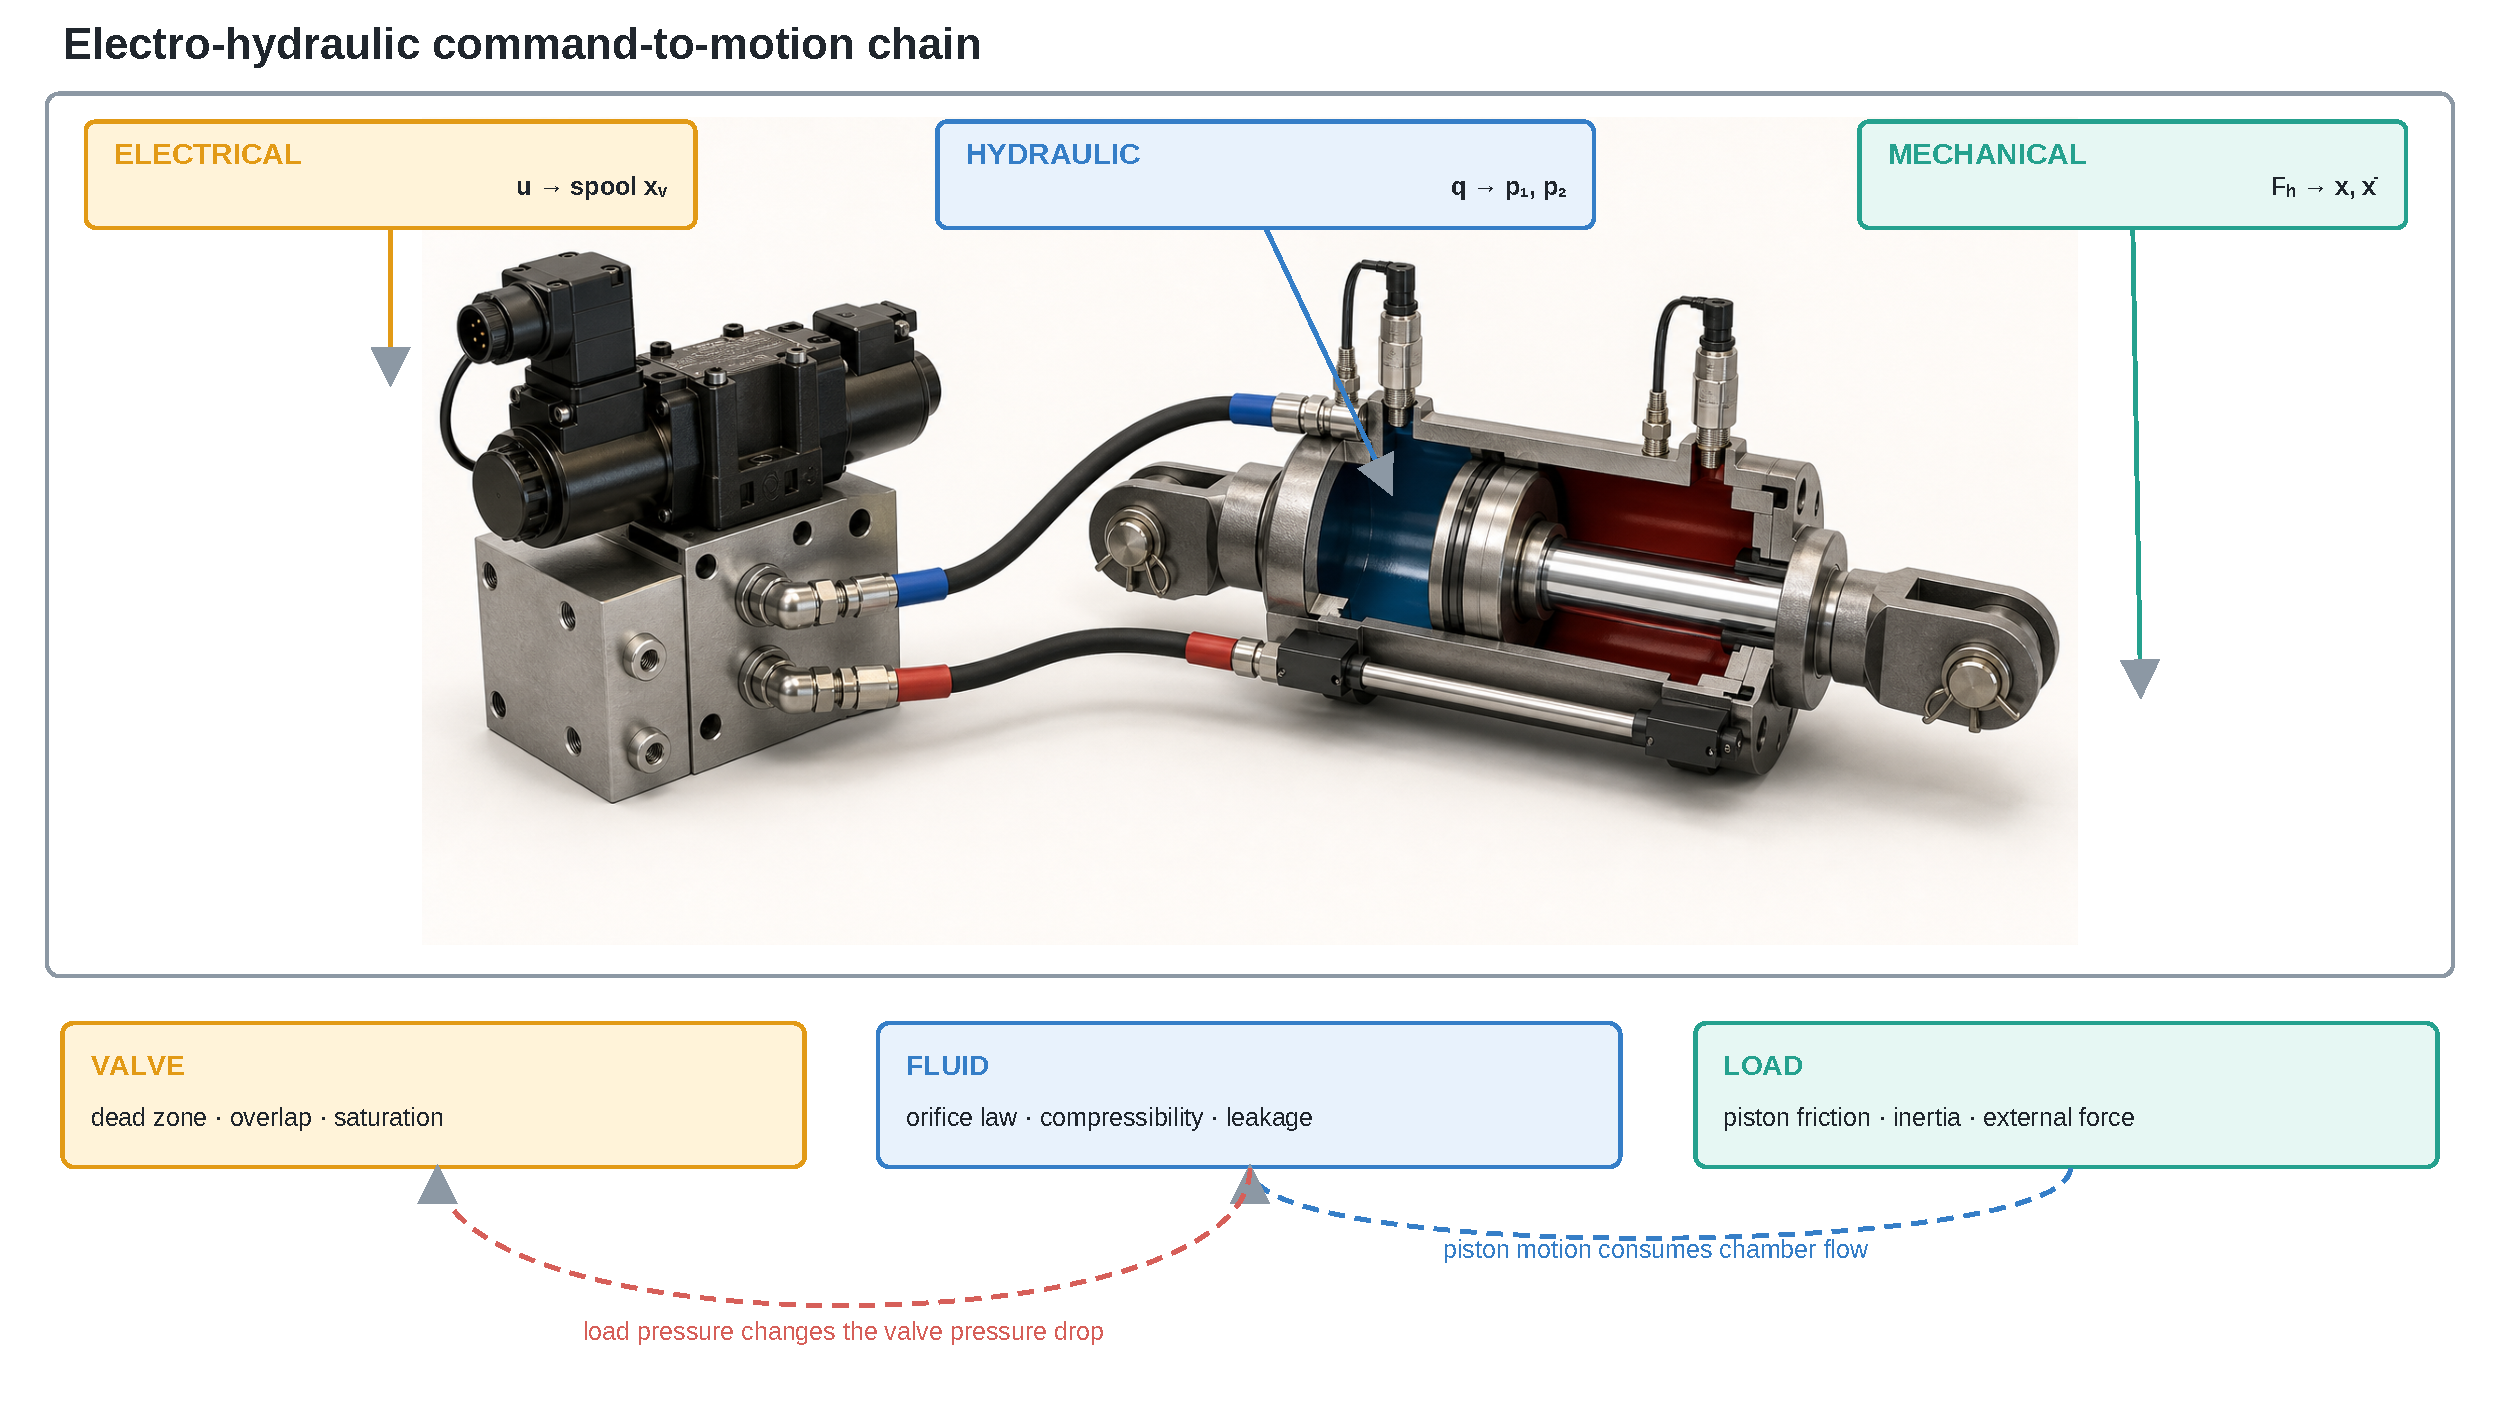
\includegraphics[width=\textwidth]{images/fund_actuation_chain}
  \caption{The electro-hydraulic actuation chain from valve command to
  mowing-head motion, grouped by energy domain. Tags beneath each domain name
  its dominant nonlinearities. The dashed return paths are the feedback loops
  that make the chain gain an operating point rather than a constant.}
  \label{fig:fund:chain}
\end{figure}

Figure~\ref{fig:fund:chain} traces the signal path that every command to
the arm must traverse. A normalized electrical command displaces the
spool of a proportional valve, which opens metering orifices toward the
supply and tank lines. To first approximation the resulting flow follows the orifice
law~\cite{merritt1967hydraulic}, in which the flow through the valve is
proportional to the spool position and to the square root of the pressure
difference across the metering edge, scaled by the discharge coefficient and
the orifice area gradient. The form is written out in
Section~\ref{sec:sys:simscape} with the coefficient values used by the plant
model. Two of its properties shape everything that follows in this thesis.
First, the flow gain depends on the square root of the pressure margin. The same spool
displacement therefore moves the cylinder quickly under light load and
barely at all when the load pressure approaches supply. The effective
valve authority is an operating point, not a constant. Second, the
relation is directional. Extending against gravity and retracting with it
see different pressure margins and hence different gains. Around the
spool null, machining overlap produces a dead zone in which small
commands move nothing at all, and at the other end of the stroke the
spool saturates~\cite{jelali2003hydraulic}.

The delivered flow does not translate directly into motion either. Oil
is compressible, the more so when air is entrained, so each cylinder
chamber acts as a nonlinear spring. Its stiffness scales with the
effective bulk modulus and inversely with the chamber volume, and the
volume itself changes with piston position. Pressure relief valves clip
the dynamics whenever a load spike or an aggressive command drives a
chamber to its limit, which happens routinely in mowing when the head
rests on the ground. Internal leakage bleeds pressure between chambers,
seal friction opposes motion, and the load pressure feeds back into the
valve flow through the orifice law. Taken together, this is the
plant that the learned models of this thesis must represent: several
interacting nonlinearities, some of them non-smooth (relief, dead zone,
stiction), and parameters such as bulk modulus, leakage, and friction
that drift with temperature and wear.

One structural point matters for the control architecture. The chain in
Figure~\ref{fig:fund:chain} ends in the mechanical linkage, where
cylinder translation becomes joint rotation through lever arms that vary
with configuration. Uncertainty entering at the valve is therefore
filtered, amplified, and coupled by the mechanism before it appears as
head-position error. This is why the models of Chapter~\ref{chap:models}
are formulated in \emph{cylinder space}, directly across the hydraulic
conversion stages, rather than in task space where hydraulic and
kinematic effects blur together.

\subsection{High-Fidelity Simulation as a Data Source}
\label{sec:fund:sim-data-source}

The hydraulic subsystems above can be modeled in detail in
component-level simulation environments such as
Simscape~\cite{mathworks2024simscape}, and Chapter~\ref{chap:data} builds
on such a model of the FME~500 arm. It is tempting to close the loop and
train a reinforcement-learning policy directly against this model, but
the computational profiles do not match. The stiff pressure dynamics
force small integration steps, and the solver processes one machine
instance at a time, while modern policy optimization spreads its sample
cost over thousands of plants simulated in parallel on a
GPU~\cite{makoviychuk2021isaac}. This thesis resolves
the mismatch by separation: the high-fidelity model is used offline as a
data generator, and compact learned representations of the actuator
carry its behavior into the parallel training environment. How this
workflow fits together is shown later, in
Figure~\ref{fig:fund:workflow}, once its ingredients have been
introduced.

\section{Kinematics and Task-Space Tracking}
\label{sec:fund:kinematics}

\subsection{Differential Kinematics}

The mowing task is specified where the work happens, as a reference path
for the cutter in vehicle coordinates. Task-space control therefore rests
on the differential kinematics of the arm~\cite{siciliano2009robotics},
in which the manipulator Jacobian maps joint rates to tool velocity and
its inverse yields the commands realizing a desired tool motion. The
plain pseudo-inverse is fragile near singular configurations, which this
arm visits routinely with the boom almost fully folded. The standard
remedy, adopted unchanged here, is the damped least-squares inverse of
Wampler~\cite{wampler1986manipulator} and Nakamura and
Hanafusa~\cite{nakamura1986inverse}, which trades bounded tracking
accuracy for bounded joint commands. It is conservative, well understood
and cheap, which are the properties wanted in a layer that must never
misbehave.

\subsection{From Joint Space to Cylinder Space}

Two complications specific to a hydraulic boom carry into the rest of the
thesis. The actuated coordinates are cylinder lengths rather than joint
angles, and each cylinder closes a triangle over its joint, so the
cylinder-to-joint map is nonlinear and its lever arm varies over the
stroke. The Jacobian used for control is therefore the composition of the
task Jacobian with that map, and an error in one cylinder's realized
motion appears in the task error of the whole arm. A passive fifth joint
coupled to the head further constrains which task directions can be
controlled independently. Chapter~\ref{chap:system} works out both
consequences and states the calibrated cutter Jacobian used throughout.

The kinematic layer, however accurate, assumes that a commanded cylinder
velocity is a realized one. Section~\ref{sec:fund:actuation-chain} argues
against that assumption on this actuator class. The kinematic controller
is therefore a \emph{nominal} structure whose commands the hydraulic
layer may or may not realize, and the learned models of this thesis live
in that realization gap.

\section{Model-Based and Conventional Control Approaches}
\label{sec:fund:conventional-control}

Industrial practice on machines like the FME~500 is open-loop operator
control: the joystick maps to valve current and the human closes every
loop. The control literature offers a spectrum of alternatives, none of which
alone settles the problem addressed here.

Classical cascade structures, an outer position loop commanding an inner
velocity or pressure loop with fixed PI or PD gains, are the workhorse of
hydraulic servo control~\cite{jelali2003hydraulic}. They are simple and
robust, but fixed gains must be tuned for the worst case across the
operating envelope, and Section~\ref{sec:fund:actuation-chain} showed
that the plant gain varies by an order of magnitude across that
envelope. The result is a controller that is sluggish where the plant is
weak or oscillatory where it is strong. On a boom whose lever arms change
with every meter of reach, one gain set cannot be right everywhere.

Model-based nonlinear methods attack the problem directly.
Computed-torque control cancels the rigid-body dynamics if they are
known~\cite{slotine1991applied}, backstepping designs extend the idea
through the pressure dynamics, adaptive versions estimate uncertain
parameters online~\cite{astrom1995adaptive}, and robust versions bound
their effect. The line remains active: Yang et
al.~\cite{yang2026stateconstrained} pair a state-constrained controller
with an explicit inverse of the valve dead-band, holding positioning
accuracy while keeping the states inside prescribed bounds. That work is
the model-based counterpart of a choice made in
Chapter~\ref{chap:models}, where the same dead-band is represented by a
learnable smooth element inside the reduced-order model rather than
inverted analytically. Applied to hydraulic manipulators these designs
achieve impressive tracking in laboratory settings, but their guarantees
are conditioned on structural model knowledge: valve flow curves,
friction models, inertia parameters. That knowledge is expensive to obtain and to maintain for a commercial
implement that is produced in variants and worked across seasons. Mattila et
al.~\cite{mattila2017survey} close their survey on the same point: model-based
hydraulic control is only as accurate as its models, and the models are the
bottleneck.

This thesis draws a specific lesson from that literature rather than
discarding it. Structured controllers are kept where structure is
reliable. The kinematic DLS layer of Section~\ref{sec:fund:kinematics}
is retained, because differential kinematics \emph{is} accurately known.
It serves as the privileged teacher that generates safe excitation and
supervises policy distillation, and as the closed-loop controller used
during identification data collection. Learning is directed at the part
where first-principles modeling is the bottleneck, the mapping between
cylinder-space commands and realized cylinder motion, and at the
task-level controller that issues those commands
(Section~\ref{sec:fund:rl-residual}). The architecture is hybrid by
design, not black-box.

\section{Data-Driven System Identification and Learned Dynamics}
\label{sec:fund:learned-dynamics}

\subsection{Learned Forward and Inverse Dynamics}

Where deriving a model is the bottleneck, one can measure it instead. In
robot model learning~\cite{nguyentuong2011model}, two complementary
mappings are distinguished. A \emph{forward dynamics} model predicts the next state, or state
increment, from the current state and the applied command, and an
\emph{inverse dynamics} model predicts the command that realizes a desired
transition. Both contracts are stated precisely in
Section~\ref{sec:models:overview}, where they are fixed for the rest of the
thesis.
Neural networks are the standard function class when the underlying
physics is non-smooth and history dependent, as it is here. For control, one-step accuracy is necessary but not sufficient. A model used inside a planner or a training loop is iterated, feeding its
own prediction back as input, so small one-step errors compound over the
horizon. A model selected purely by one-step loss can diverge within a few
hundred milliseconds of recursive prediction~\cite{nagabandi2018neural}.
Multi-step rollout objectives, which iterate the model during training and
penalize the accumulated error, counteract this compounding directly and
are used for every dynamic model trained in this thesis. The
probabilistic-ensemble line of work~\cite{chua2018deep} addresses the
same problem by additionally tracking how model uncertainty grows along
the rollout. Where a single sample cannot summarize the relevant past,
for instance pressure transients and valve history, recurrent
architectures~\cite{hochreiter1997long,cho2014learning} extend
the forward model with an internal state that integrates a window of
history. The reduced-order model of Chapter~\ref{chap:models} takes this
form.

\subsection{Closed-Loop Identifiability}
\label{sec:fund:identifiability}

The dominant practical danger in learning a forward model is not
underfitting but learning the wrong thing well. System-identification
theory has long formalized when data determines a plant: informative
experiments require inputs that excite the dynamics independently of the
feedback law~\cite{ljung1999system,isermann2011identification}. Data
collected in closed loop violates this in a treacherous way. The
controller computes the command from the state history, so command and
state are strongly correlated, and a flexible model can reach excellent
prediction scores by exploiting the state history alone. It then behaves
like a sophisticated persistence model that ignores the input channel.
The failure is silent, because validation data from the same closed-loop
distribution keeps rewarding the shortcut. Schoukens and
Ljung~\cite{schoukens2019nonlinear} emphasize that for nonlinear systems
the design of informative excitation is, if anything, more critical than
for linear ones.

This is not a hypothetical concern in this thesis. It is a measured
event. The first forward-dynamics model of Chapter~\ref{chap:models},
trained on closed-loop operation data, reached one-step $R^2$ near
$0.999$ while an input ablation showed that it had learned almost no
dependence on the valve command at all. The open-loop excitation
campaign of Chapter~\ref{chap:data}, valve sequences applied directly
to the plant without any feedback controller in the loop, exists
specifically to break this correlation and make the causal
valve-to-motion path identifiable. The methodological rule that follows is applied to every
learned model in this work: input-ablation tests with zeroed and
shuffled commands are part of model acceptance, and a supervised score
is never accepted as evidence of control authority on its own.

\section{Reduced-Order Modeling}
\label{sec:fund:rom}

The term \emph{reduced-order model} comes from a literature on projecting
high-dimensional dynamical systems onto low-dimensional subspaces that
preserve their dominant behavior, surveyed with its parametric variants by
Benner et al.~\cite{benner2015survey}. The motivation carries over directly:
a model cheap enough to evaluate thousands of times per second, yet faithful
enough that conclusions drawn from it transfer. Here the construction is
learned rather than projected, reducing the full Simscape hydraulic model to
a compact per-cylinder state of extension, extension velocity and pressure
difference.

Between white-box projection and black-box regression lies the grey-box
middle ground this thesis occupies. Physics-informed learning embeds known
structure into the hypothesis class so that data is spent on what is
unknown~\cite{karniadakis2021physics}, an approach Lutter et
al.~\cite{lutter2019deep} demonstrated for rigid-body dynamics by building
Lagrangian structure into a network. The reduced-order model of
Chapter~\ref{chap:models} applies this to hydraulics: the orifice law, the
pressure-buildup equation and the integrator chain are explicit layers with
trainable effective parameters, while neural components supply only the valve
realization, the configuration-dependent load and small bounded residuals.
Two properties motivated this over a free-form sequence model. The trained
parameters can be checked for physical plausibility, and the bounded
residuals prevent an off-distribution input from producing an unphysical
state jump, which matters in a policy-training loop that pushes its model
off-distribution by design.

The closest precedent for embedding such a surrogate in policy training
comes from legged robotics. Hwangbo et
al.~\cite{hwangbo2019learning} identified the rigid-body mechanics of
their robot analytically, learned the response of its series-elastic
actuators from measured data, trained a policy against the resulting
hybrid simulation, and deployed it directly on the machine. Later work industrialized this recipe in GPU-parallel
simulators~\cite{rudin2022learning}. Yamamori et
al.~\cite{yamamori2026actuator} have since inverted the premise, shaping the
physical actuator's closed-loop response to match the idealized dynamics
assumed in simulation. That option is unavailable on a commercial implement
carrier whose valve and pump are not open to redesign, which is why the
modeling burden here falls on the actuator representation.
Figure~\ref{fig:fund:workflow} shows the same division of labor recast for
hydraulics. The PhysX articulation plays the analytic rigid-body part, and
the learned part is not a torque filter for a well-behaved electric drive but
the entire hydraulic chain of Figure~\ref{fig:fund:chain}. The surrogate must
therefore be hydraulic-aware and command-conditioned, realizing desired
cylinder commands rather than filtering torques.

\begin{figure}[tb]
  \centering
  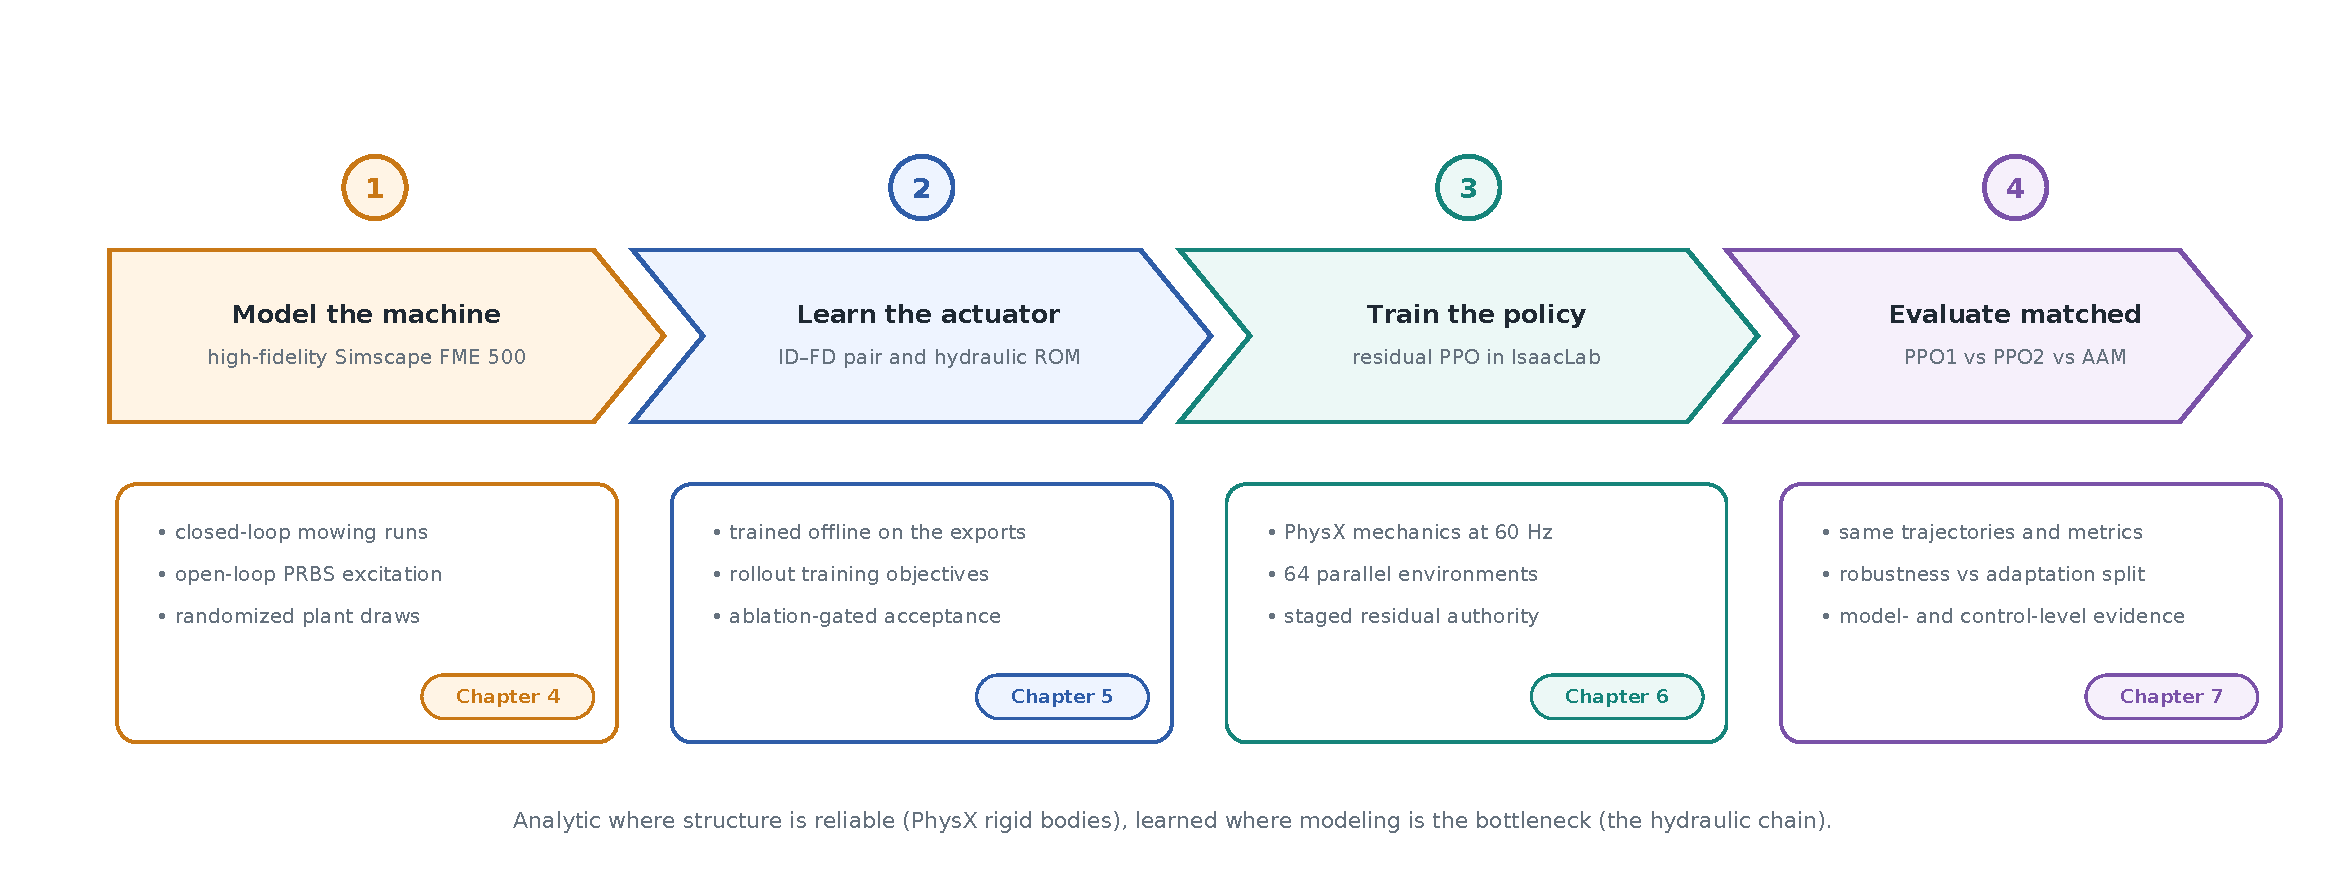
\includegraphics[width=\textwidth]{images/fund_workflow}
  \caption{The four-step workflow of this thesis, following the
  division of labor introduced for legged robots by Hwangbo et
  al.~\cite{hwangbo2019learning}. Each card names what the step contributes and
  the chapter that develops it.}
  \label{fig:fund:workflow}
\end{figure}

\section{Domain Randomization and Latent Adaptation}
\label{sec:fund:domain-randomization}

\subsection{Robustness Through Randomized Training}

A model or policy trained on one simulated plant inherits every
parameter of that plant as an implicit assumption. Domain randomization
attacks this brittleness by training across a distribution of plants,
originally over visual appearance for
perception~\cite{tobin2017domain}, soon after over dynamics parameters
such as masses, frictions, gains, and latencies for
control~\cite{peng2018sim}. The now-standard reading of those results is
that a policy or model that must succeed on many plants converges to
behavior that is \emph{robust} across the family. For the hydraulic arm
the corresponding family is physically meaningful rather than
synthetic: effective bulk modulus varies with entrained air and
temperature, valve gains and leakage drift with wear, and payload
changes with the mounted attachment. Chapter~\ref{chap:data} defines the
randomized parameter space along these same axes.

\subsection{From Robustness to Adaptation}

\begin{figure}[tb]
  \centering
  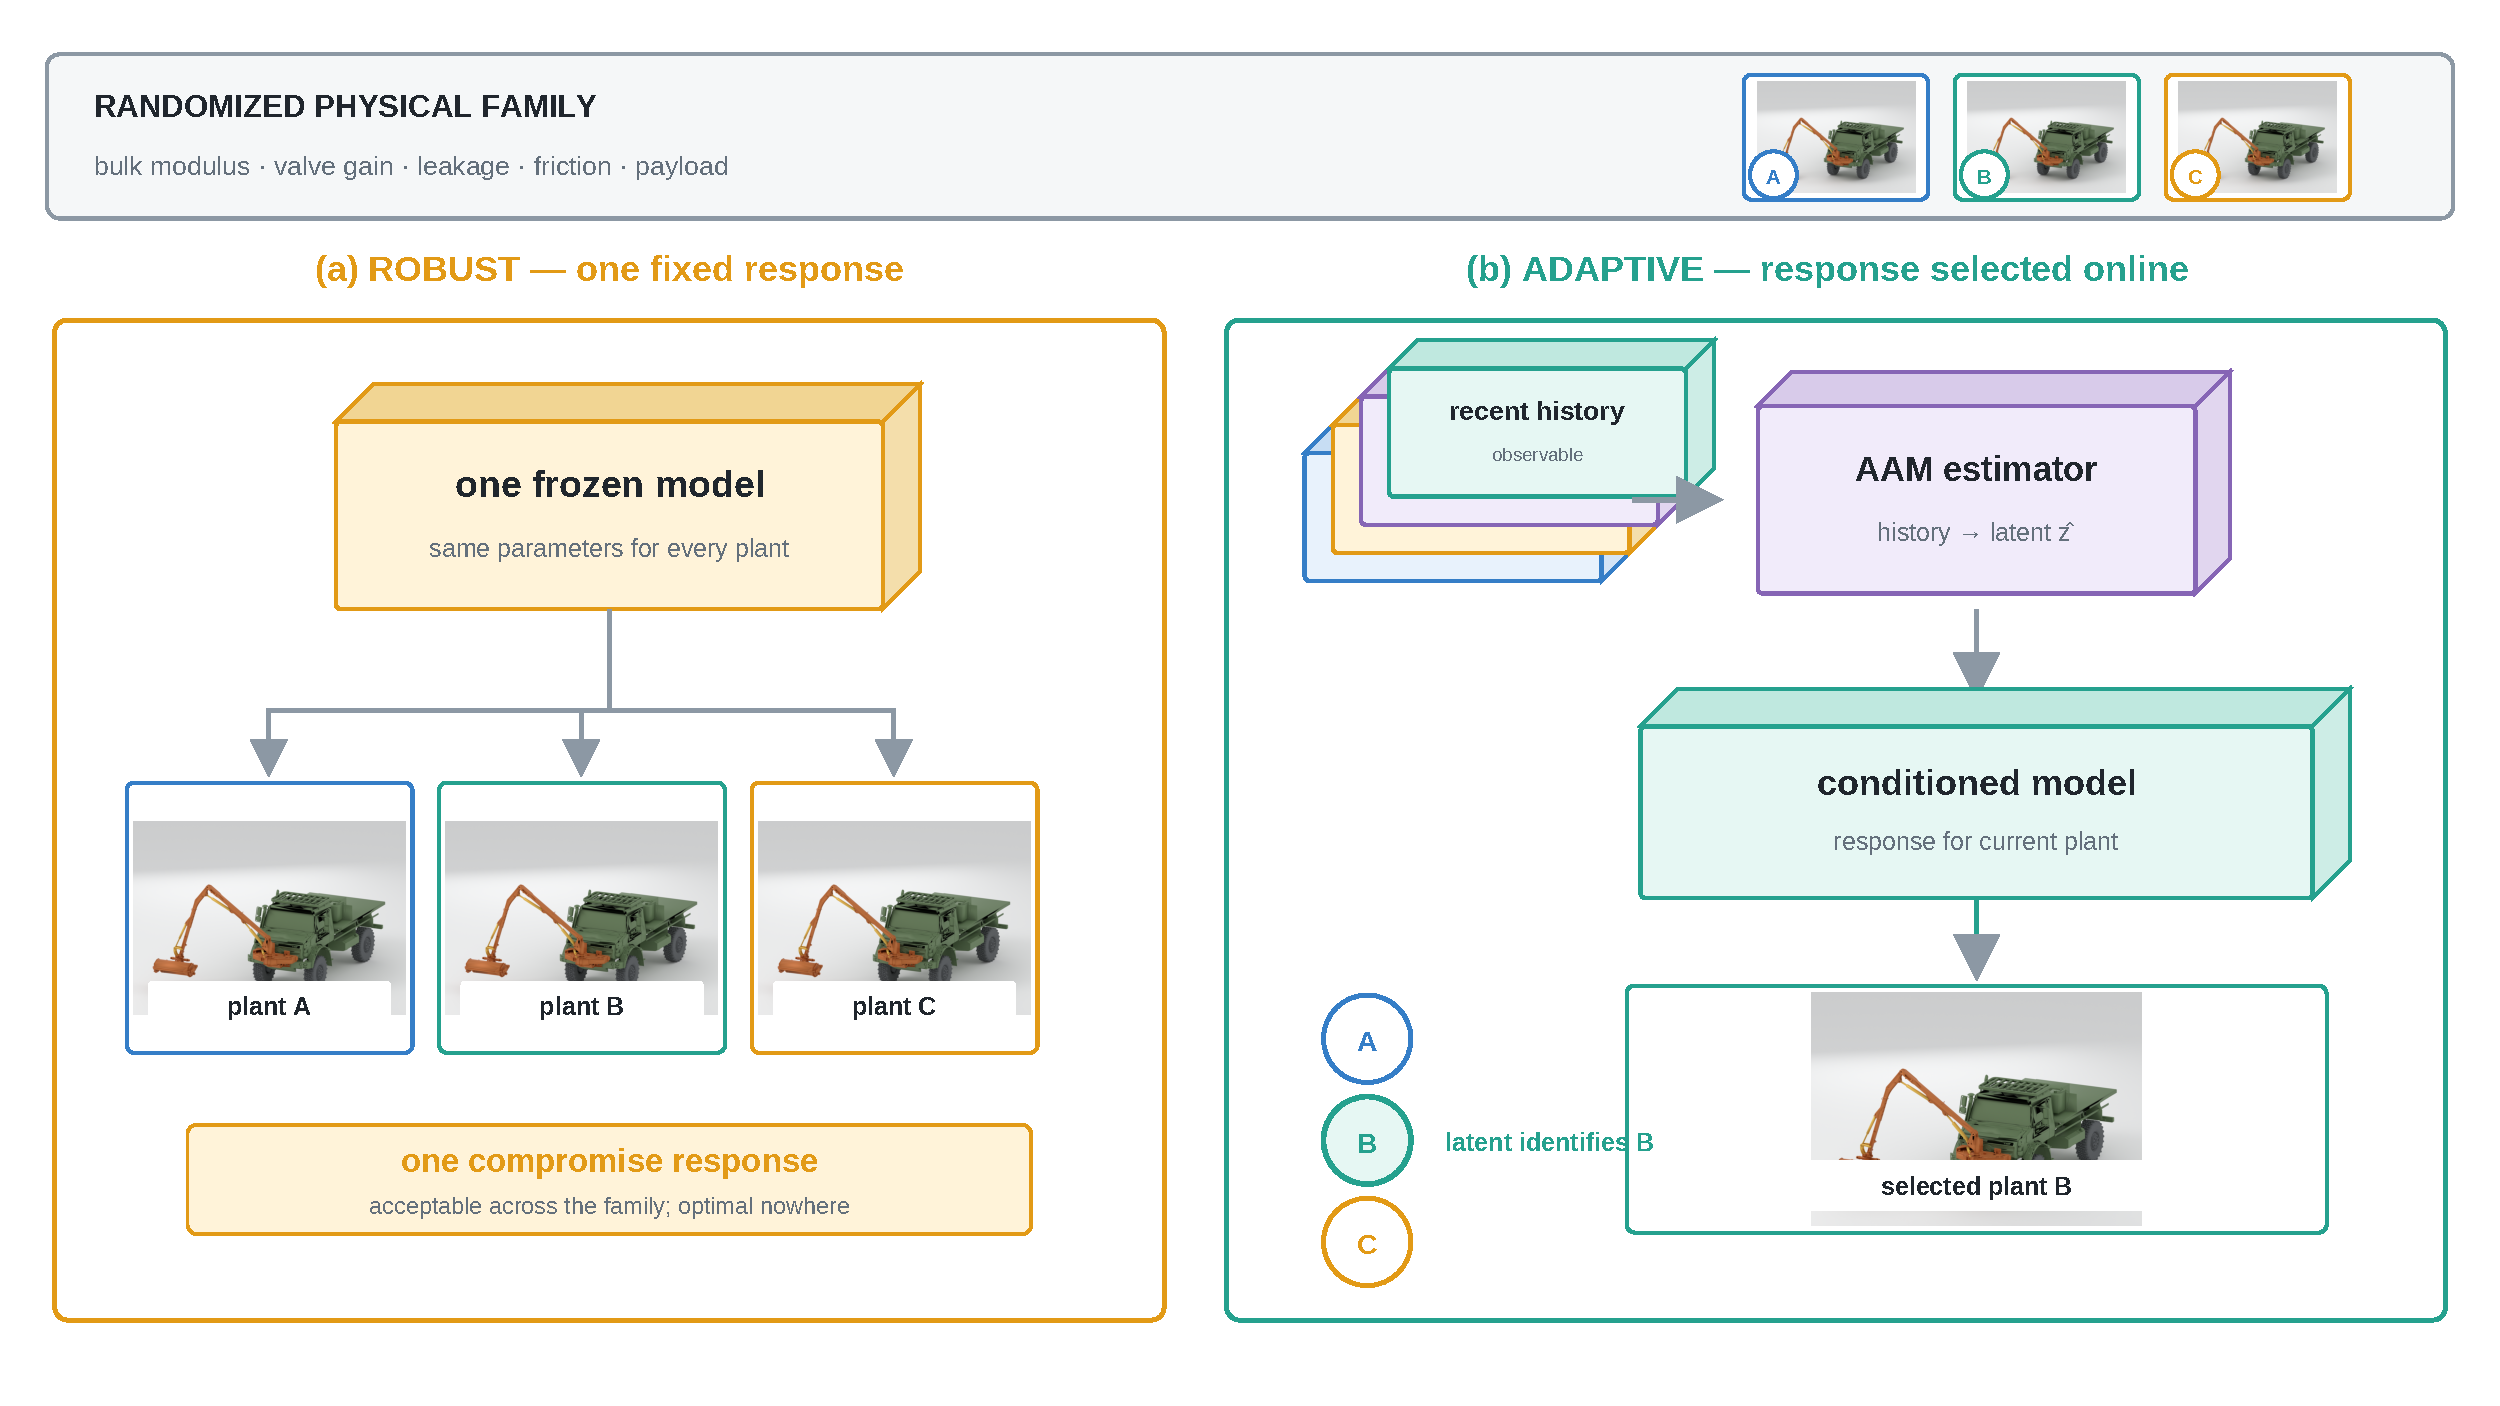
\includegraphics[width=\textwidth]{images/fund_robust_adaptive}
  \caption{Two treatments of the same randomized plant
  family. (a)~Randomized training alone gives a \emph{robust} model: one fixed
  response, acceptable everywhere and optimal nowhere. (b)~Latent conditioning
  adds \emph{adaptation}: an estimator infers $\hat{\bm{z}}$ from recent
  measured history and the model changes its response. The estimator is trained
  against a privileged latent but deploys on observable signals alone.}
  \label{fig:fund:robust-adaptive}
\end{figure}

Robustness, however, is a compromise by definition: one response that is
acceptable everywhere is optimal nowhere. The alternative is to let the
controller or model identify which member of the family it is currently
facing and condition on that estimate
(Figure~\ref{fig:fund:robust-adaptive}). The teacher--student
construction makes this trainable. During simulation the true randomized
factors $\factorvec$ are known, and a privileged encoder compresses
them, or their dynamic consequences, into a low-dimensional latent
$\bm{z}$. A
student module then learns to regress $\bm{z}$ from signals that exist
outside simulation, namely the recent history of states, commands, and
responses. Lee et al.~\cite{lee2020learning} used this scheme to walk
over terrain whose properties the robot cannot observe directly. Kumar et al.~\cite{kumar2021rma} sharpened it into rapid motor adaptation.
A first phase trains the policy together with an encoder of the privileged
environment parameters. A second phase trains an adaptation module to recover
the same latent from the observable state--action history. At deployment only
the history-based estimate is used, so the system adapts within fractions of a
second and takes no gradient steps. Classical adaptive control pursues the same goal through online
parameter estimation~\cite{astrom1995adaptive}. The learned variant
replaces explicit parameter estimates with a task-shaped latent, trading
physical interpretability for the ability to summarize many interacting
parameters at once. The construction has since been carried into the
dynamics model itself rather than the policy. Yu et
al.~\cite{yu2026context} condition a neural-ODE dynamics model on a
context vector inferred from state--action history, so the learned model
rather than the controller is what adapts to the current plant. That is
the position the AAM occupies here, and the reason this thesis measures
the adaptation effect at the actuator layer instead of inside the
policy.

The Arm Adaptation Module (AAM) of this thesis
(Chapter~\ref{chap:models}) is this construction applied to hydraulic
actuation, following the adaptive path of
Figure~\ref{fig:fund:robust-adaptive}(b). The privileged latent
$\bm{z} = \mu(\factorvec)$ is a two-dimensional compression of the
physical factor vector $\factorvec$, validated by the system-dynamics
surrogate of Chapter~\ref{chap:models}. The AAM reads its deployable
estimate $\latenthat$ from a quarter second of causal, observable
cylinder-signal history.

Where that estimate is \emph{used} is a design decision that this thesis
fixes explicitly, because it is easy to state loosely. The latent does
not condition the reduced-order model. In the proposed stack,
\ppoIDAAMFD, the inferred latent conditions a small bounded residual
adapter around the \emph{frozen inverse-dynamics model}, leaving the
forward model, the policy, and the PhysX plant unchanged. Conditioning
the policy directly on $\latenthat$ is treated as an ablation rather
than the default design (Chapter~\ref{chap:evaluation}). Two claims are
therefore kept apart throughout. A model trained across randomized
plants is \emph{robust}, not automatically adaptive, and evidence that a
\emph{privileged} latent carries useful dynamics information is not
evidence that an \emph{inferred} one improves control. Collapsing either
pair is a common confound in the sim-to-real literature, and the
experimental design of Chapter~\ref{chap:evaluation} is built to avoid
both.

\section{Reinforcement Learning and Structured Priors}
\label{sec:fund:rl-residual}

\subsection{Policy Optimization}

Reinforcement learning frames control as sequential decision making: a
policy $\pi_\vartheta(\bm{a}\,|\,\bm{o})$ maps observations to actions
and is optimized to maximize expected cumulated
reward~\cite{sutton2018reinforcement}. Among policy-gradient methods,
proximal policy optimization (PPO)~\cite{schulman2017proximal} has
become the default in robot learning for its simplicity and stable
large-batch behavior. It constrains each update through a clipped surrogate objective, which
limits how far the ratio between the new and the old policy may move before
the improvement term stops paying. Advantages are estimated with generalized
advantage estimation~\cite{schulman2016gae}. The objective as configured for
this thesis is written out in Section~\ref{sec:ctrl:optimization}. What makes
on-policy methods like PPO practical for this thesis is throughput.
GPU-parallel simulators run thousands of environment instances at
once~\cite{makoviychuk2021isaac}, and locomotion policies have been
trained this way in minutes~\cite{rudin2022learning}. This is the regime
in which the full hydraulic model cannot run
(Section~\ref{sec:fund:sim-data-source}) and the learned actuator
surrogates can.

\subsection{Structured Priors for Policy Learning}
\label{sec:fund:prior}

Applying RL to the mowing arm from scratch would discard the reliable
kinematic structure of Section~\ref{sec:fund:kinematics} and force the policy
to rediscover it from reward, with excursions a heavy boom cannot afford.
Three constructions inject that structure, and they differ in \emph{when} the
classical controller acts.

Residual reinforcement learning adds the policy output to a hand-designed
controller's command at
runtime~\cite{johannink2019residual,silver2018residual}, with the policy
restricted to a bounded band. The nominal controller provides competent
behavior from the first step, but it remains in the deployed loop, so every
result is a property of the pair. Policy distillation moves the prior to
training time instead: a privileged teacher, here the DLS controller reading
quantities the deployed system cannot, generates demonstrations, and the
student is fitted to them by supervised imitation before any reward is
optimized~\cite{ross2011reduction}. At deployment the teacher is gone and the
student is the whole controller. The third construction, developed in
Section~\ref{sec:ctrl:anchored}, keeps the prior for the whole of
optimization without returning it to the runtime loop. The distilled student
is frozen as a \emph{reference} policy and reward optimization is restricted
to a neighbourhood of it, measured as a divergence between the two action
distributions and evaluated only on states the learner itself visits.

This thesis uses the second and third. The deployed policy of all three
stacks is a \emph{sole} cylinder-motion controller, emitting the desired
cylinder command with no nominal command added at runtime, and the DLS
controller is retained only as teacher and as the closed-loop controller
during identification. What bounds exploration is therefore not a residual
band but the action contract itself, specified in
Chapter~\ref{chap:control}.

Improving a policy that a simulator has already made competent is an active
question. Yin et al.~\cite{yin2025rapidly} retain the value function learned
in simulation to guide exploration during real-world fine-tuning, treating
the simulator as a source of structure rather than a plant to be abandoned.
This thesis shares that premise and differs in what is retained: the policy
itself, held as a fixed reference that bounds how far reward optimization may
travel.

That construction answers a measured result rather than a design assumption.
\emph{Unconstrained} PPO fine-tuning from the distilled student raised total
reward while degrading the primary tracking objective, consistently enough
that distillation was for several development cycles treated as the
\emph{endpoint} rather than an initialization. The diagnosis is a mismatch of
objectives rather than a failure of the optimizer: the reward is a proxy,
acceptance is decided by physical gates, and the reward's optimum does not
lie inside the gate-feasible set (Section~\ref{sec:ctrl:training}). Anchoring
is what allows the reported \ppoROM{} policy to be a fine-tuned actor rather
than a distilled one.

\subsection{Reinforcement Learning on Hydraulic Machines}

Applications of deep RL to hydraulically actuated arms are still few,
and the closest of them sharpen rather than close the gap this thesis
addresses. Egli and Hutter demonstrated RL-based trajectory tracking for
the arm of a full-size hydraulic excavator, first in
simulation-to-machine transfer experiments~\cite{egli2020towards} and
then as a general automation approach deployed on a walking
excavator~\cite{egli2022general}. Spinelli et
al.~\cite{spinelli2024rl} extended that line to material handlers whose
tool is underactuated, training in simulation and validating on a
commercial machine, which shows the approach scales to arms where part
of the mechanism is not directly commanded. The mowing head of this
thesis is underactuated in the same sense, through its passive swivel
joint. Maitan et al.~\cite{maitan2026contraction} attacked the problem
from the opposite end, learning force control for a single hydraulic
actuator directly on hardware and constraining exploration with a
contraction-metric filter so that training on a real cylinder stays
safe. Their work is the closest published statement of the difficulty
this thesis handles in simulation: an unconstrained policy acting on a
hydraulic cylinder is not safe by default, and something must bound it.
Their key ingredient is shared with
this work: a data-driven model of the machine's actuator response,
learned from recorded operation and used as the training plant for the
policy. The differences define where this thesis stands. Their actuator
model is identified for one physical machine, so robustness across a
plant family and online adaptation to a changing plant are outside its
scope. Their policy is trained against that single model without a
privileged teacher supplying the structured prior. And their evaluation
compares against human operators and classical baselines rather than
isolating the contribution of the actuator representation itself. The
comparison that Chapter~\ref{chap:evaluation} is built around (same task, same policy architecture, same observation and action contracts,
same terrain, reward, seeds and training budget, with only the actuator and adaptation path differing) has to the author's knowledge no
published counterpart for hydraulic manipulators.

One property of a learned policy over a learned actuator cuts both ways
and shapes the evaluation methodology of this thesis. Because the policy
can compensate for a mediocre actuator model, closed-loop tracking error
alone cannot distinguish a good model from a good patch over a bad one.
The protocol of Chapter~\ref{chap:evaluation} therefore reports
model-level rollout metrics, the magnitude and smoothness of the emitted
commands, and the standing cylinder-tracking and actuator-prediction
residuals alongside task error. A better actuator representation must show up as a smaller standing model error and
quieter commands, not merely as equal tracking.

\section{Research Gap and Thesis Positioning}
\label{sec:fund:gap}

Laid side by side, the threads of this chapter each solve part of the
problem and leave a specific remainder
(Table~\ref{tab:fund:positioning} names the works). Hydraulic control
theory provides structure and explains why fixed models fail, but its
precise methods presuppose plant knowledge that a commercial mowing
implement does not come with. Learned dynamics models replace
derivation with data, but the identifiability literature, and the
measured failure recounted in Section~\ref{sec:fund:identifiability},
shows that closed-loop operation data silently produces models without
control authority. Learned actuator surrogates embedded in parallel
simulation are proven for electric drives but not for actuators
dominated by pressure dynamics, relief saturation, and valve dead
zones. Domain randomization yields robustness, and the teacher--student
construction yields fast online adaptation, but these results live
almost entirely in locomotion, where the adapted quantity is the
contact with the world rather than the actuator itself. RL has reached
full-size hydraulic arms, but without a structured prior, without
adaptation, and without isolating the actuator representation.
Residual RL and policy distillation both integrate learning with a
structured controller, yet published evaluations rarely control for the
fact that the policy can mask actuator-model deficiencies.

\begin{table}[tb]
  \centering
  \caption{Positioning of this thesis against the reviewed lines of work.
  Columns: (I)~learned model of \emph{hydraulic} actuator dynamics;
  (II)~training data audited for causal input identifiability;
  (III)~online latent adaptation to a changing plant; (IV)~structured
  classical controller retained as a prior, with bounded action
  authority; (V)~matched comparison isolating the actuator
  representation.
  ($\checkmark$)~=~partially or implicitly addressed.}
  \label{tab:fund:positioning}
  \small
  \begin{tabular}{lccccc}
    \toprule
    Line of work & I & II & III & IV & V \\
    \midrule
    Model-based hydraulic control~\cite{mattila2017survey,jelali2003hydraulic}
      & --- & ($\checkmark$) & ($\checkmark$) & $\checkmark$ & --- \\
    Actuator networks for legged robots~\cite{hwangbo2019learning,rudin2022learning,yamamori2026actuator}
      & --- & $\checkmark$ & --- & --- & --- \\
    RL for hydraulic machines~\cite{egli2020towards,egli2022general,spinelli2024rl,maitan2026contraction}
      & $\checkmark$ & ($\checkmark$) & --- & --- & --- \\
    Latent online adaptation~\cite{lee2020learning,kumar2021rma,yu2026context}
      & --- & --- & $\checkmark$ & --- & --- \\
    Residual RL and policy
    distillation~\cite{johannink2019residual,silver2018residual,ross2011reduction,yin2025rapidly}
      & --- & --- & --- & $\checkmark$ & --- \\
    \midrule
    This thesis (\ppoROM{} / \ppoIDFD{} / \ppoIDAAMFD)
      & $\checkmark$ & $\checkmark$ & $\checkmark$ & $\checkmark$ & $\checkmark$ \\
    \bottomrule
  \end{tabular}
\end{table}

What is missing is the combination, summarized in
Table~\ref{tab:fund:positioning}: cylinder-space actuator dynamics learned
from deliberately identifiable data, reduced to a physics-structured
command-conditioned model fast enough for massively parallel policy
training, carrying a dynamics latent that is validated before deployment
and recovered online from observable history alone, and evaluated in a
framework where adaptive and non-adaptive actuator representations are
compared under matched conditions. Assembling this on the MULAG FME~500
mowing arm is the contribution of this thesis. It takes the form of three
control stacks differing \emph{only} in the actuation and adaptation path
between the policy's cylinder command and PhysX:

\begin{description}
  \item[\ppoROM.] The policy commands desired cylinder motion, which the
    validated command-conditioned reduced-order model realizes. This is
    the certified actuator baseline and the current shippable stack.
  \item[\ppoIDFD.] The same policy interface drives the frozen inverse
    model followed by the validated strict forward model. This is the
    non-adaptive learned baseline. It tracks the line more finely than
    \ppoROM{} and fails the ground-contact requirement, which makes it an informative negative result rather than a weaker copy.
  \item[\ppoIDAAMFD.] The AAM infers a dynamics latent from causal
    observable history, and that latent conditions a small bounded
    residual adapter around the frozen inverse model before the same
    frozen forward model and PhysX. This is the proposed adaptive
    method.
\end{description}

The scientific variable is therefore the actuator and adaptation path
alone, with task, observation and action contracts, terrain, reward,
training budget, test factors, seeds and acceptance gates held matched.
Robustness and adaptation are measured as separate effects rather than
conflated ones. The next chapter grounds this program in the concrete
system.

%%%%%%%%%%%%%%%%%%%%%%%%%%%%%%%%%%%%%%%%%%%%%%%%%%%%%%%%%%%%
%% Chapter 3 — System Fundamentals and Problem Formulation
%% (10–15 pages)
%% Purpose: describe the physical and simulated system once,
%% define all coordinate spaces and interfaces, and formulate
%% the control objective mathematically.
%%%%%%%%%%%%%%%%%%%%%%%%%%%%%%%%%%%%%%%%%%%%%%%%%%%%%%%%%%%%
\chapter{System Fundamentals and Problem Formulation}
\label{chap:system}

Chapter~\ref{chap:fundamentals} closed with a program: learn the
hydraulic actuation of the FME~500 from identifiable data, wrap the
learned models in a structured controller, and measure robustness and
adaptation as separate effects. Before any of that can be made concrete,
the system itself has to be pinned down. This chapter describes the
manipulator and its two simulated representations exactly once, so that
every later chapter can refer back here instead of re-explaining the
plant. Sections~\ref{sec:sys:platform} and~\ref{sec:sys:kinematics}
define the mechanism, its coordinate spaces, and the mappings between
them. Section~\ref{sec:sys:actuation} fixes which signals exist, which
are commanded, and which are merely estimated.
Section~\ref{sec:sys:simscape} summarizes the high-fidelity Simscape
model that generated the historical actuator-model data, and
Section~\ref{sec:sys:isaaclab} the IsaacLab environment in which
policies are trained, adaptation data is collected, and every result in
this thesis is measured. Section~\ref{sec:sys:task} defines the verge-following task and the actuator
ceiling that constrains it. Section~\ref{sec:sys:architecture} assembles the
control architecture and the three stacks that differ inside it.
Sections~\ref{sec:sys:problem} and~\ref{sec:sys:evaluation-criteria} state the
control problem and the criteria the thesis is judged by.

\section{Manipulator Platform}
\label{sec:sys:platform}

The MULAG FME~500 is modeled as a serial-link manipulator with five
revolute joints. Figure~\ref{fig:sys:topology} shows the kinematic
topology. The chain starts at the base frame bolted to the Unimog's
front attachment plate (link~0), continues through the slew column
(link~1), the two boom segments (links~2 and~3), and the head carrier
(link~4), and ends in the flail mowing head (link~5). Four double-acting
hydraulic cylinders actuate the first four joints. Each cylinder closes
a triangle over its joint, so cylinder extension and joint angle are
related through the linkage geometry. The fifth joint, the rotation of
the mowing head itself, carries no cylinder of its own in the
configurations studied here: it is constrained by a swivel-link
mechanism coupled to the head carrier, and the control task treats it as
passive. Throughout the thesis the four actuated cylinders are indexed
in the fixed order introduced in Chapter~\ref{chap:models}: slew
(\emph{Drehzapfen}), boom~I (\emph{Ausleger~I}), boom~II
(\emph{Ausleger~II}), and head pivot (\emph{Messerkopf-Schwenk}).

\begin{figure}[tb]
  \centering
  \begin{subfigure}[b]{.58\linewidth}
    \centering
    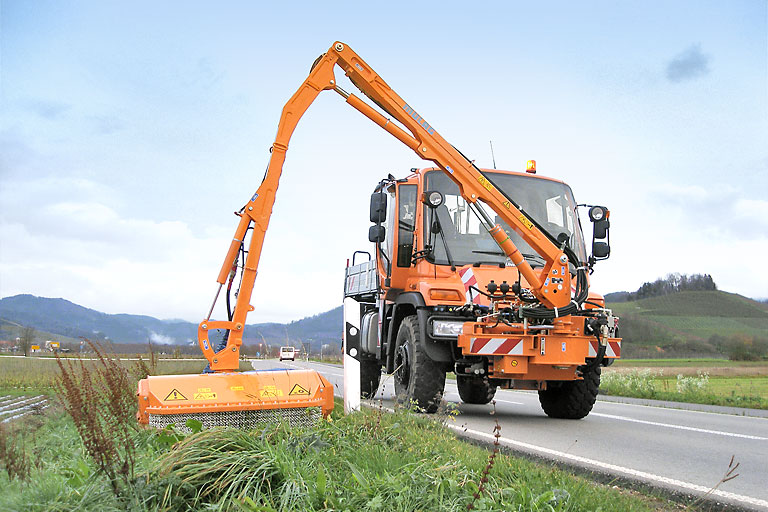
\includegraphics[width=\linewidth]{images/fme500_operation}
    \caption{}
    \label{fig:sys:fme500-photo}
  \end{subfigure}
  \hfill
  \begin{subfigure}[b]{.38\linewidth}
    \centering
    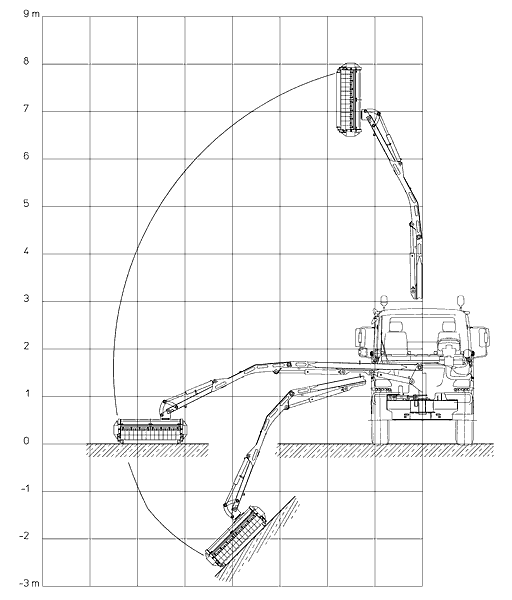
\includegraphics[width=.82\linewidth]{images/fme500_reach_diagram}
    \caption{}
    \label{fig:sys:fme500-reach}
  \end{subfigure}
  \caption{The machine studied in this thesis, as delivered.
  (a)~MULAG FME~500 front mower on a Unimog carrier during roadside mowing.
  (b)~Manufacturer's working envelope, spanning roughly $\unit[8]{m}$ of height
  and reaching below road level. Images: MULAG
  Fahrzeugwerk~\cite{mulag2024fme500}.}
  \label{fig:sys:fme500}
\end{figure}

\begin{figure}[tb]
  \centering
  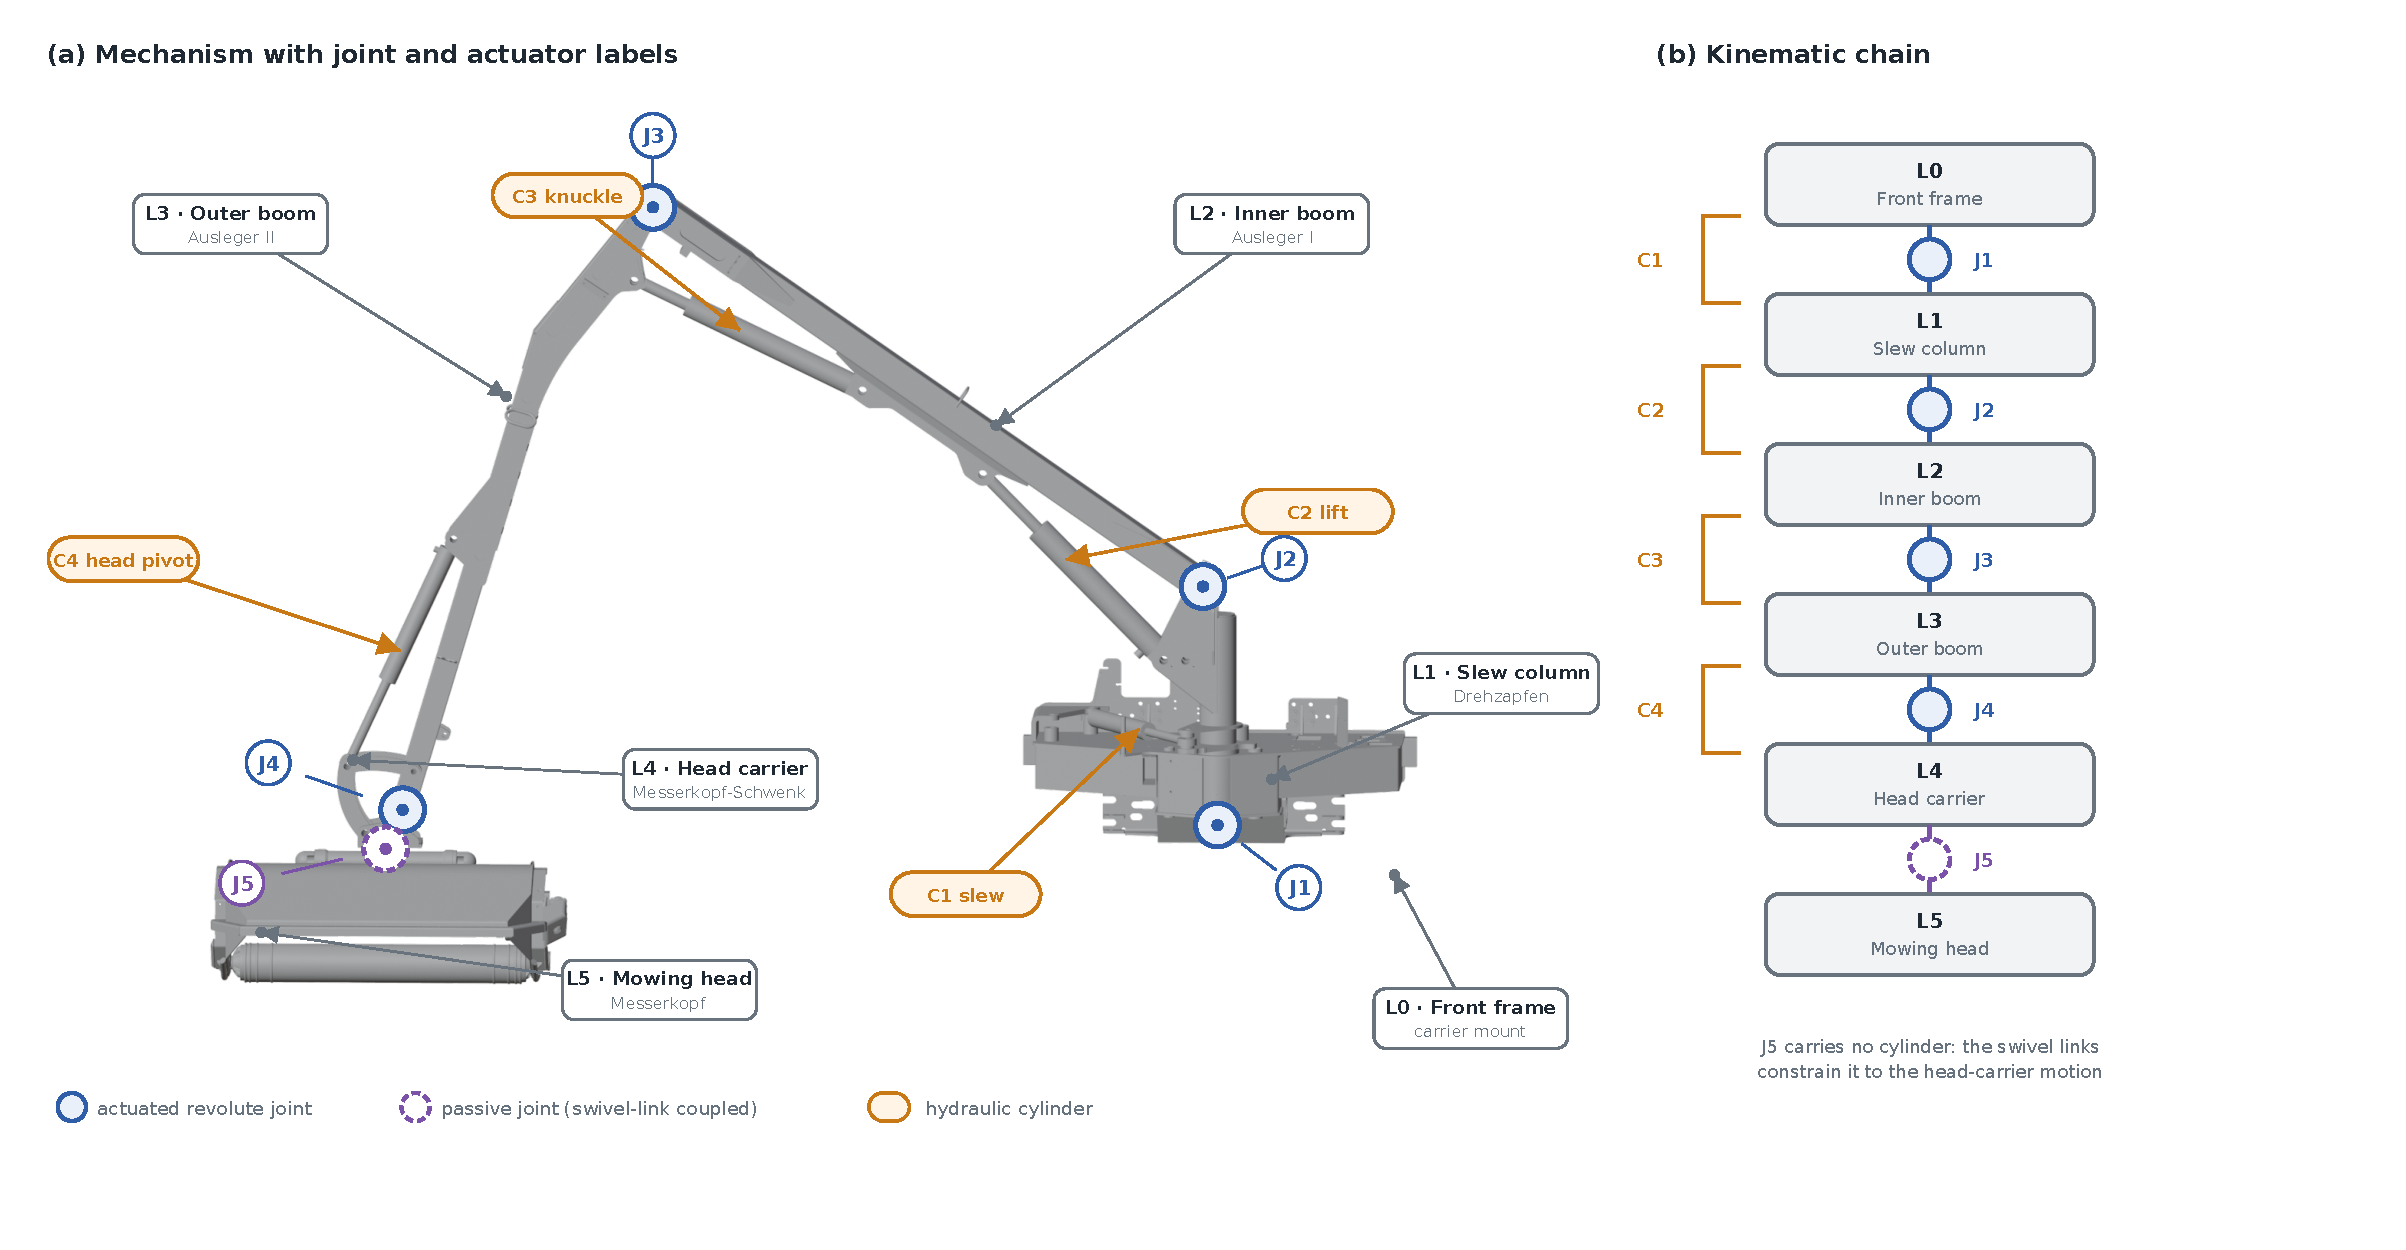
\includegraphics[width=\textwidth]{images/fme500_topology_annotated}
  \caption{Kinematic topology of the MULAG FME~500, rendered from
  the CAD model. (a)~The mechanism with every link (L0--L5), joint (J1--J5) and
  cylinder (C1--C4) called out; J5 is dashed to mark it passive. (b)~The same
  structure as an abstract chain, with the passive fifth joint coupled through
  swivel links rather than a cylinder.}
  \label{fig:sys:topology}
\end{figure}

The geometry is not hand-approximated. Link shapes, masses, centers of
mass, and full inertia tensors were extracted from the manufacturer's
CAD data using the Blender add-on
Phobos~\cite{vonszadkowski2020phobos}, which exports a consistent URDF
description of the mechanism. This matters for a machine like the
FME~500: the boom is a long, asymmetric weldment whose cross-inertia
terms are significant, and a lumped-mass approximation would
misrepresent the very load coupling that makes the hydraulics hard to
control. The same CAD-derived description is the common ancestor of
both simulated representations used in this thesis, the Simscape model
of Section~\ref{sec:sys:simscape} and the IsaacLab articulation of
Section~\ref{sec:sys:isaaclab}, so their mechanical parameters agree by
construction.

Table~\ref{tab:sys:cylinders} lists the actuated joints and the
extension ranges of their cylinders as observed across the training
data. Two geometric facts recur throughout the thesis. First, the
controlled point is not the origin of the head body: the cutter contact
point sits $\unit[0.79]{m}$ below the \emph{Messerkopf} body origin,
and all task-space errors are measured at this offset tool tip. Second,
the mowing pose of interest keeps the head facing straight down. The
head-pivot cylinder holds a dedicated reference extension
($\unit[0.589]{m}$) to maintain this orientation, which effectively
reserves the fourth cylinder for the orientation task and leaves
cylinders~1--3 for positioning.

\begin{table}[tb]
  \centering
  \caption{Actuated joints of the modeled FME~500 and the extension
  ranges of their cylinders observed in the training data
  (Chapter~\ref{chap:data}).}
  \label{tab:sys:cylinders}
  \begin{tabular}{clcc}
    \toprule
    $i$ & Joint (German designation) & Function & Extension range [m] \\
    \midrule
    1 & \emph{Drehzapfen}         & slew about vertical axis & $0.018$ -- $0.493$ \\
    2 & \emph{Ausleger I}         & inner boom elevation     & $0.275$ -- $0.791$ \\
    3 & \emph{Ausleger II}        & outer boom articulation  & $0.309$ -- $0.857$ \\
    4 & \emph{Messerkopf-Schwenk} & head pivot (orientation) & $0.269$ -- $0.689$ \\
    \midrule
    5 & \emph{Messerkopf}         & head rotation, passive (swivel links) & --- \\
    \bottomrule
  \end{tabular}
\end{table}

\section{Kinematic Structure and Coordinate Mappings}
\label{sec:sys:kinematics}

\subsection{Joint Space and Cylinder Space}

The mechanism's configuration is described by the joint vector
$\bm{q} \in \mathbb{R}^5$ and its velocity $\dot{\bm{q}}$. The actuated
coordinates, however, are the cylinder extensions
$\bm{x} \in \mathbb{R}^4$ introduced in Chapter~\ref{chap:models}. Each
cylinder connects an attachment point $\bm{p}_A$ on link $k$ to a point
$\bm{p}_B$ on link $k{+}1$, both fixed in their links and exported from
the CAD data. The instantaneous cylinder length and extension are
%
\begin{equation}
  \label{eq:sys:cyl-length}
  \ell_i(\bm{q}) = \bigl\| \bm{p}_B(\bm{q}) - \bm{p}_A(\bm{q}) \bigr\|,
  \qquad
  x_i = \ell_i(\bm{q}) - \ell_{0,i},
\end{equation}
%
with $\ell_{0,i}$ the retracted reference length. Differentiating
\eqref{eq:sys:cyl-length} gives the scalar mapping between joint motion
and extension rate,
%
\begin{equation}
  \label{eq:sys:cyl-jac}
  \dot{x}_i = J_{\mathrm{cyl},i}(\bm{q})\, \dot{\bm{q}},
  \qquad
  J_{\mathrm{cyl},i} = \bm{e}_i^{\!\top}
  \bigl( \bm{J}_B - \bm{J}_A \bigr),
\end{equation}
%
where $\bm{e}_i$ is the unit vector along the cylinder axis and
$\bm{J}_A, \bm{J}_B$ are the translational Jacobians of the attachment
points. The same mapping carries force back to torque: by the principle
of virtual work, a cylinder force $F_{h,i}$ contributes the joint
torque $\bm{\tau}_{\mathrm{act}} = \bm{J}_{\mathrm{cyl}}^{\top}
\bm{F}_h$. The rows of $\bm{J}_{\mathrm{cyl}}$ are the lever arms
discussed qualitatively in Chapter~\ref{chap:fundamentals}. They vary
over the stroke, and with them the effective gain and stiffness that
each cylinder presents to its joint.

\subsection{Task Space and the Calibrated Cutter Jacobian}
\label{sec:sys:task-jacobian}

The task is defined at the cutter tip, expressed in the truck chassis
frame (\texttt{base\_link}). This choice is deliberate and matters in
practice: the articulation root of the simulated arm is the slew base,
which moves with the arm, and using it as the reference frame corrupts
every tracking measurement. All references and errors in this thesis
live in the truck frame, and the controlled point includes the
$\unit[-0.79]{m}$ tool-tip offset of Section~\ref{sec:sys:platform}.
Because the truck itself drives forward during the primary task
(Section~\ref{sec:sys:task}), the chassis frame translates along the
road while the errors are measured inside it. The along-track direction
is supplied by the vehicle and is not a controlled degree of freedom.

For control, the composition of task kinematics and cylinder linkage is
captured in a single calibrated Jacobian
$\bm{J}_c \in \mathbb{R}^{3\times4}$ that maps cylinder extension rates
to cutter-tip velocity in the truck frame. Rather than deriving it
symbolically through the CAD chain, it was measured directly on the
simulated plant: starting from the head-down mowing configuration, each
cylinder target was stepped in turn and the settled cutter displacement
recorded, giving central-difference estimates of every column. The
measured matrix has rank~3 with singular values $8.24$, $5.69$, and
$2.79$, confirming that at the mowing operating point the four
cylinders span exactly three independent task directions. This is the
quantitative form of the observation from
Section~\ref{sec:sys:platform}: with cylinder~4 committed to holding
the head down, the remaining freedom moves the cutter in a
three-dimensional workspace, and one direction of the nominal base
frame is reachable only through vehicle motion. The damped
least-squares controller of Chapter~\ref{chap:control} inverts this measured $\bm{J}_c$, so the nominal layer and the plant share one
geometric contract.

\section{Actuation and Measured State}
\label{sec:sys:actuation}

Every interface in this thesis draws from one signal inventory, and it is stated once here, together with who can see what.
Table~\ref{tab:sys:signals} summarizes the quantities, their
dimensions, and their availability in the two simulation environments.

\begin{table}[tb]
  \centering
  \caption{Signal inventory of the modeled system. ``S'' marks signals
  present in the Simscape data exports, ``I'' signals available live in
  the IsaacLab environment, ``M'' quantities that exist there only
  through the learned models of Chapter~\ref{chap:models}, and ``P''
  \emph{privileged} quantities that exist in simulation but must never
  enter a deployable policy or estimator input.}
  \label{tab:sys:signals}
  \small
  \begin{tabular}{llcl}
    \toprule
    Signal & Dimension & Availability & Meaning \\
    \midrule
    $\bm{u}$ & $[-1,1]^4$ & S, M & normalized proportional-valve commands \\
    $\bm{x},\, \dot{\bm{x}}$ & $\mathbb{R}^4$ & S, I & cylinder extensions and velocities \\
    $\Delta\bm{p}$ & $\mathbb{R}^4$ & S, M & chamber pressure differences \\
    $\bm{F}$ & $\mathbb{R}^4$ & S & logged rod forces \\
    $\bm{q},\, \dot{\bm{q}}$ & $\mathbb{R}^5$ & S, I & joint positions and velocities \\
    $\bm{p}_c$ & $\mathbb{R}^3$ & S, I & cutter-tip position, truck frame \\
    $\bm{h}$ & $\mathbb{R}^{9}$ & I & forward terrain-height profile ahead of the cutter \\
    $\bm{c} = [\Delta\bm{x}^*, \Delta\dot{\bm{x}}^*]$ & $\mathbb{R}^8$ & I & desired cylinder command \\
    $\factorvec$ & $\mathbb{R}^6$ & P & physical randomization factors of the active plant \\
    $\bm{z} = \mu(\factorvec)$ & $\mathbb{R}^{d_z}$ & P & privileged dynamics latent, $d_z = 2$ \\
    $\latenthat$ & $\mathbb{R}^{d_z}$ & M & AAM estimate of $\bm{z}$ from observable history \\
    \bottomrule
  \end{tabular}
\end{table}

The separation encoded in that table drives several design decisions.
The valve command $\bm{u}$ exists only inside the Simscape plant and
its data exports. In IsaacLab no valve is simulated, so any model that
needs valve information at runtime must either receive it from a
learned inverse model (the \ppoIDFD{} and \ppoIDAAMFD{} paths) or
predict it internally (the reduced-order model of the \ppoROM{} path).
The pressure difference $\Delta\bm{p}$ likewise has no native
counterpart in the rigid-body simulation. At runtime it is a recursive
internal state of the learned actuator models rather than a
measurement, and it is deliberately withheld from the deployment-mirror
inputs of Chapter~\ref{chap:models} so that the causal history estimator
cannot lean on a quantity a real machine would not publish. Only
positions and velocities, of cylinders, joints, and the cutter tip,
together with the terrain scan, are common ground, which is why the
acceptance gates of Section~\ref{sec:sys:evaluation-criteria} are formulated on these quantities.

The last three rows carry the rule that governs the whole adaptation
argument. The factor vector $\factorvec$ and the latent
$\bm{z} = \mu(\factorvec)$ derived from it are privileged: they are
known to the simulator, they are used to \emph{train} and to
\emph{audit}, and they are never read by anything that claims to be
deployable. Only $\latenthat$, inferred from causal observable history,
may enter the adaptive stack. Commanded quantities carry a star and
estimated ones a hat, following the notation of
Chapter~\ref{chap:models}; $\latenthat$ exists only in \ppoIDAAMFD.

\section{High-Fidelity Simscape Model}
\label{sec:sys:simscape}

The primary data source for the \emph{actuator} models of this thesis
(the command-conditioned reduced-order model and the inverse/forward
pair) is a multi-domain Simscape model of the FME~500 that I
developed in the master project preceding this thesis. This section
summarizes the parts of that model the thesis depends on. The modeling
and validation work itself is part of the contribution of this research
program.

The division of provenance is stated explicitly, because the data campaigns
of Chapter~\ref{chap:data} are easy to conflate and the three actuator
paths do \emph{not} share the same one.
Table~\ref{tab:sys:provenance} states it once.

\begin{table}[tb]
  \centering
  \caption{Provenance of each frozen actuator component. The command ROM
  is the only one that has been calibrated against the deployment plant;
  the inverse/forward pair is Simscape-identified throughout. This
  asymmetry is a property of the comparison and is carried into the
  discussion of Chapter~\ref{chap:evaluation}, not glossed over.}
  \label{tab:sys:provenance}
  \small
  \begin{tabular}{lp{4.4cm}p{5.0cm}}
    \toprule
    Component & Identified on & Calibrated on \\
    \midrule
    Command ROM & Simscape closed-loop export (grey-box, full model)
      & IsaacLab/PhysX closed-loop rollouts, via a bounded command-gated
        correction head only \\
    Control ID & Simscape closed-loop export & --- \\
    Strict FD & Simscape closed-loop export, retrained on the strict
        open-loop excitation export & --- \\
    $SD_0$, $\mu(\factorvec)$, $SD_z$, AAM
      & IsaacLab/PhysX adaptation collection (from scratch) & --- \\
    \bottomrule
  \end{tabular}
\end{table}

The Simscape model is therefore \emph{historical} provenance for the
bulk of every actuator model, and the sole provenance of the frozen ID
and strict FD checkpoints, which are carried forward unchanged. It is
not the whole story for the command ROM: after its Simscape training the
ROM received a small, bounded, closed-loop calibration inside IsaacLab
itself, described in Section~\ref{sec:models:rom-calibration}. And it
produced nothing at all for the adaptation chain: the system-dynamics
surrogate, the privileged factor encoder, and the AAM are trained from
scratch on data collected in IsaacLab through the command ROM and PhysX
(Section~\ref{sec:sys:isaaclab}).

\subsection{The Command ROM as Deployment Actuator}
\label{sec:sys:rom-is-plant}

One design decision governs everything downstream and is therefore stated
explicitly: \emph{the command ROM plus PhysX is the deployment plant of this
thesis}. Inside the simulator it stands in for the real machine. Simscape is
too slow to be that stand-in (Section~\ref{sec:fund:sim-data-source}) and the
bare PhysX articulation has no hydraulics, so the hydraulically structured,
PhysX-calibrated ROM is the best representation available at policy-training
throughput. That is why it alone was calibrated against the deployment loop,
and why the system-dynamics surrogate and the AAM describe \emph{it} rather
than Simscape.

The ROM therefore holds two roles at once: it is the plant, and it is the
actuator of \ppoROM. The consequence for the three-way comparison is carried
into Chapter~\ref{chap:evaluation} rather than left implicit:

\begin{itemize}
  \item \ppoROM{} is the stack whose actuator \emph{coincides with the
    plant}. It therefore measures how well the task can be done when the
    actuator model is, by construction, exactly right. It is the
    reference condition, not merely the best of three models.
  \item \ppoIDFD{} substitutes an independently identified learned
    actuator pair for that plant model. It measures the cost of that substitution: what is lost when the actuator representation is
    identified elsewhere and must reproduce the deployment plant rather
    than be it.
  \item \ppoIDAAMFD{} measures how much of that cost online adaptation
    recovers.
\end{itemize}

Read this way the ID transfer gap of Chapter~\ref{chap:evaluation} is an
expected quantity rather than an anomaly. Read carelessly, \ppoROM's advantage
looks like evidence that a reduced-order model approximates better than an
inverse--forward pair, which is \emph{not} what the experiment can show. This
qualification applies wherever \ppoROM{} is quoted as the certified
baseline.

\subsection{Mechanical Subsystem}

The mechanism is simulated as a rigid multibody system in Simscape
Multibody~\cite{mathworks2024simscape}, with the CAD-derived links,
joints, and cylinder attachment frames of
Section~\ref{sec:sys:platform}. The joint-space dynamics take the
standard manipulator form
%
\begin{equation}
  \label{eq:sys:eom}
  \bm{M}(\bm{q})\ddot{\bm{q}}
  + \bm{C}(\bm{q},\dot{\bm{q}})\dot{\bm{q}}
  + \bm{g}(\bm{q})
  + \bm{\tau}_{\mathrm{fric}}(\dot{\bm{q}})
  = \bm{\tau}_{\mathrm{act}} - \bm{J}^{\top}(\bm{q})\,\bm{F}_{\mathrm{ext}},
\end{equation}
%
with the inertia matrix $\bm{M}$ assembled from the imported CAD
tensors. Two terms deserve comment. The friction torque
$\bm{\tau}_{\mathrm{fric}}$ combines viscous and Coulomb components
with a smooth $\tanh$ approximation of the sign function, extended by a
Stribeck term at the cylinder level to capture stick--slip at low
velocities. The slew joint, which carries high side loads, is
particularly sensitive to this. The external wrench
$\bm{F}_{\mathrm{ext}}$ models the vegetation cutting load as a nominal
force plus a disturbance that scales with feed velocity and vegetation
density, rather than as a constant, so mowing does not reduce to a
static payload. Each cylinder is built as a closed kinematic loop
(spherical--prismatic--cylindrical, shown in the top band of
Figure~\ref{fig:sys:actuator-channel}), which lets it self-align under
load without over-constraining the mechanism, and hard-stop constraints
enforce the physical stroke limits of
Table~\ref{tab:sys:cylinders}.

\subsection{Hydraulic Subsystem}

\begin{figure}[tb]
  \centering
  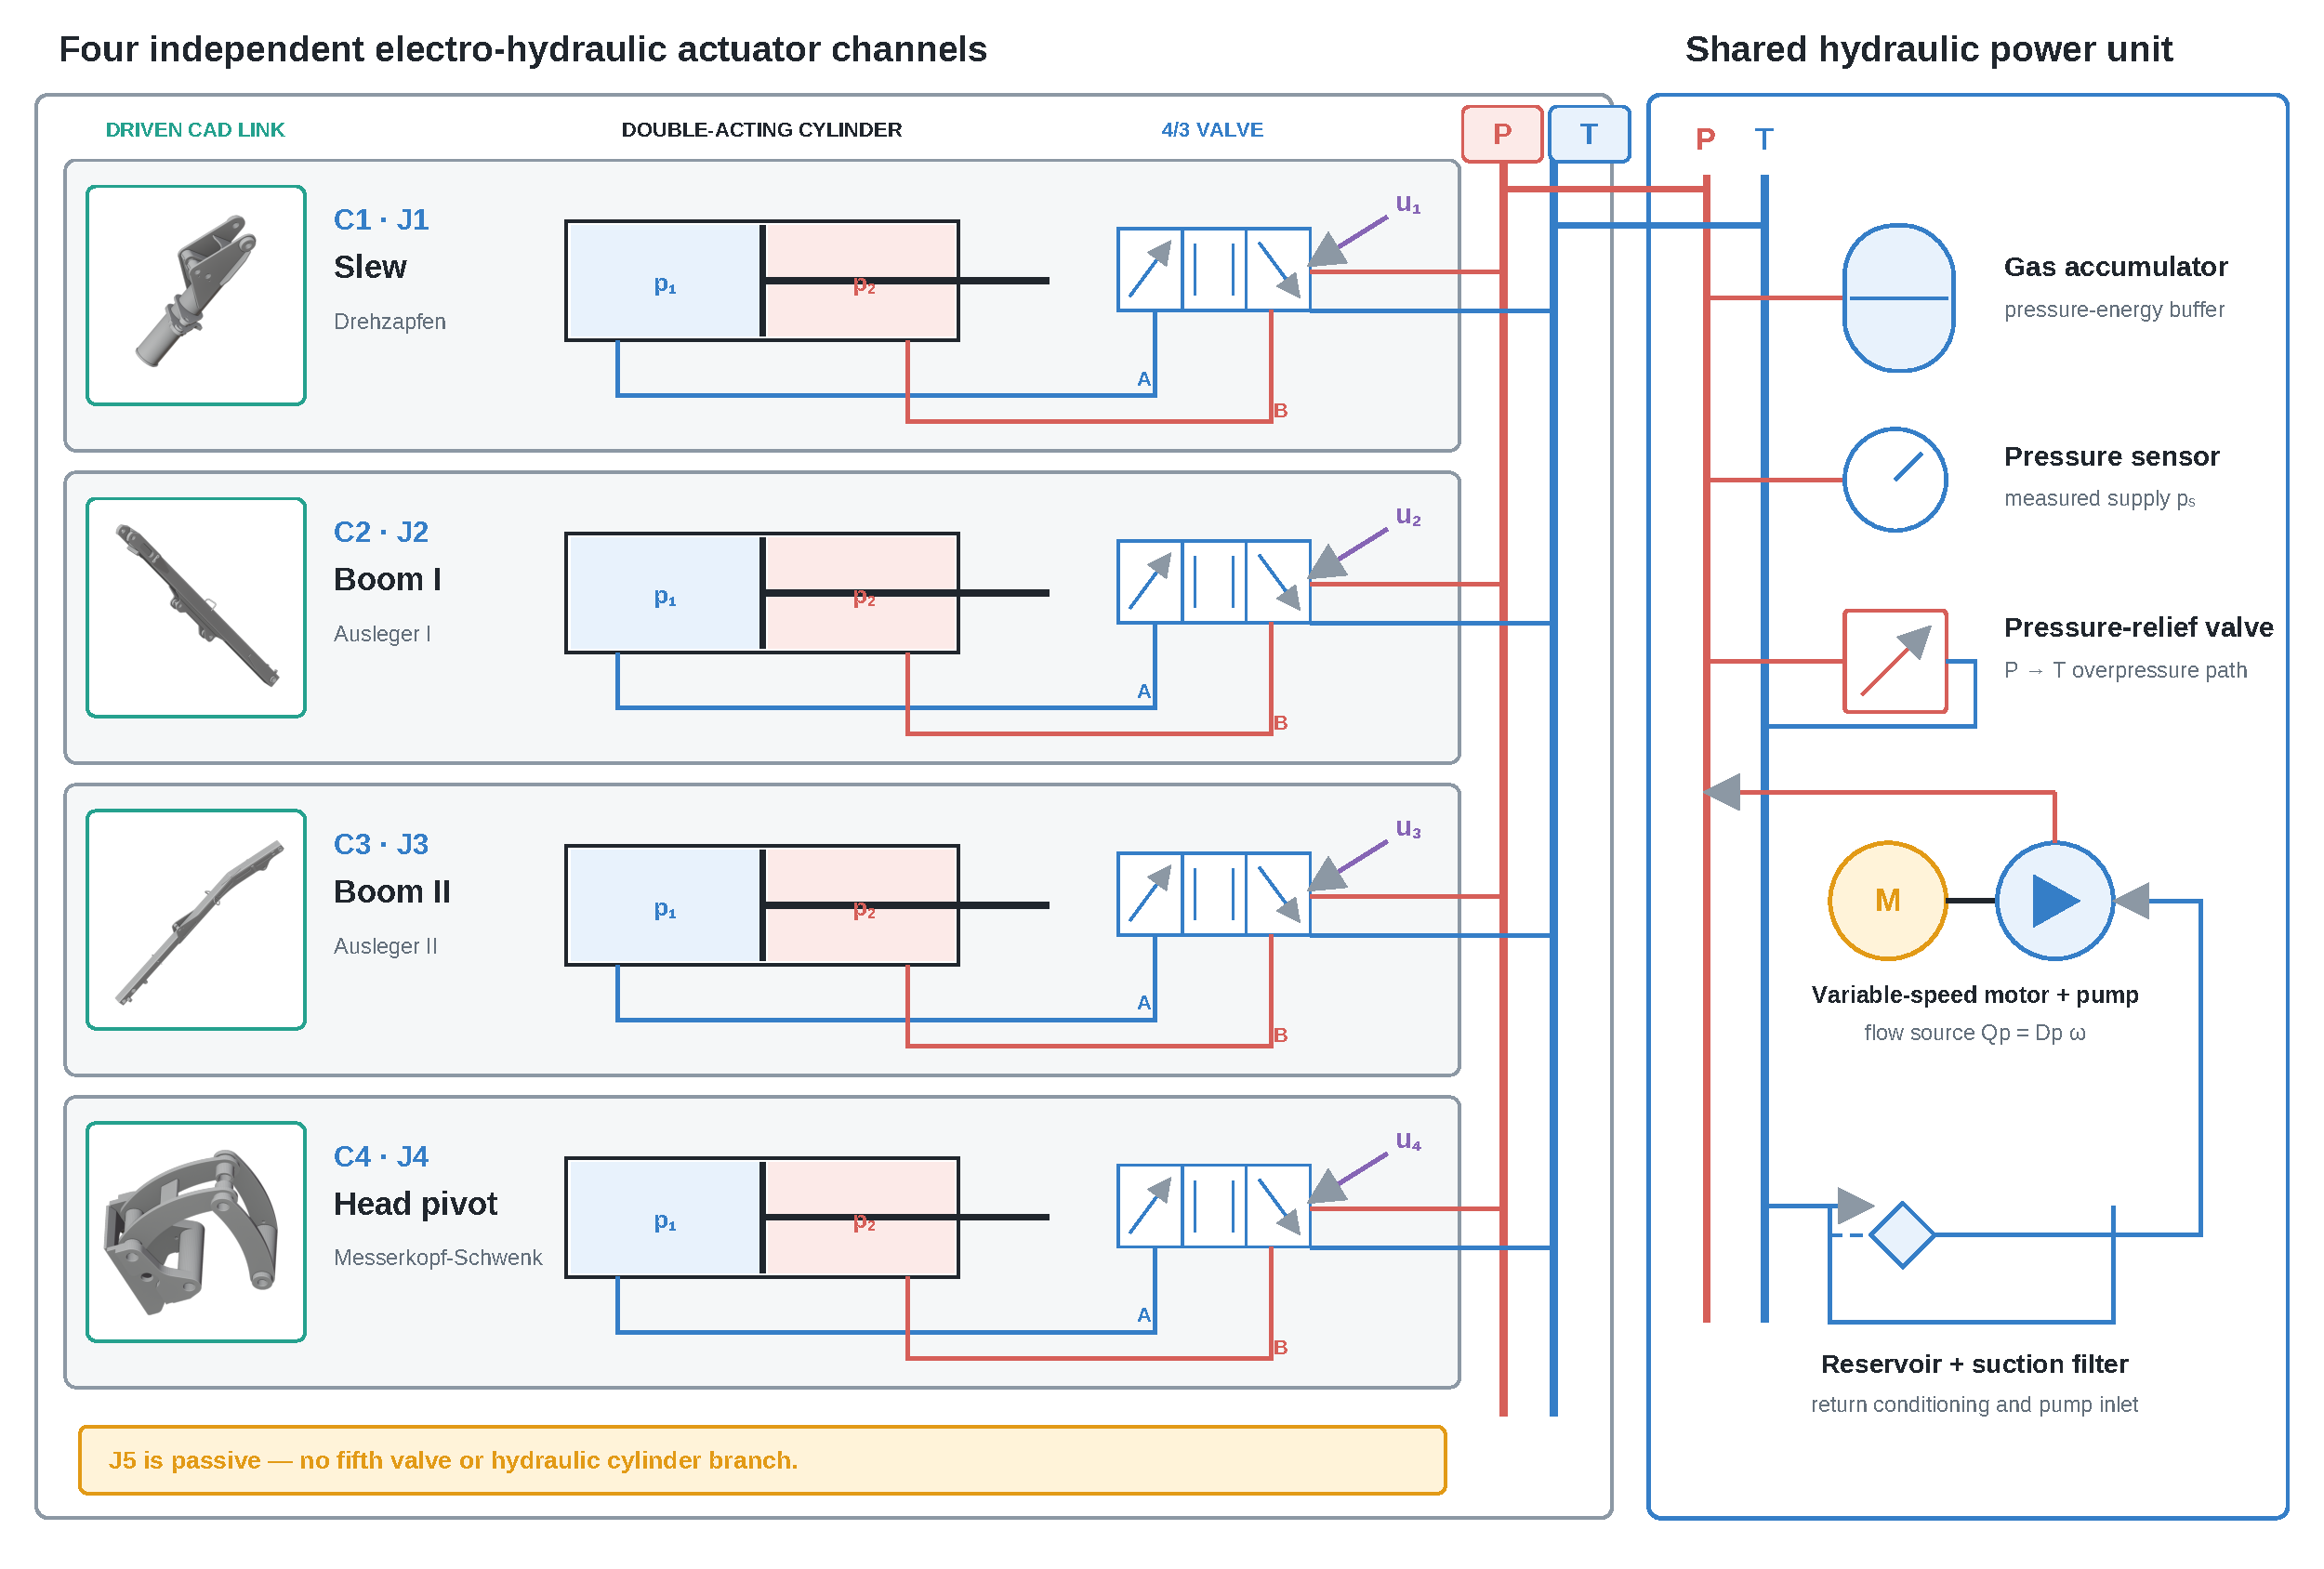
\includegraphics[width=\textwidth]{images/fme500_hydraulic_schematic}
  \caption{System-level hydraulic schematic. Left: the four
  independent actuator channels, each a 4/3 proportional directional valve
  driving one double-acting cylinder. Right: the power unit shared by all four
  channels. Link thumbnails are rendered from the CAD model of
  Figure~\ref{fig:sys:topology}.}
  \label{fig:sys:schematic}
\end{figure}

\begin{figure}[tb]
  \centering
  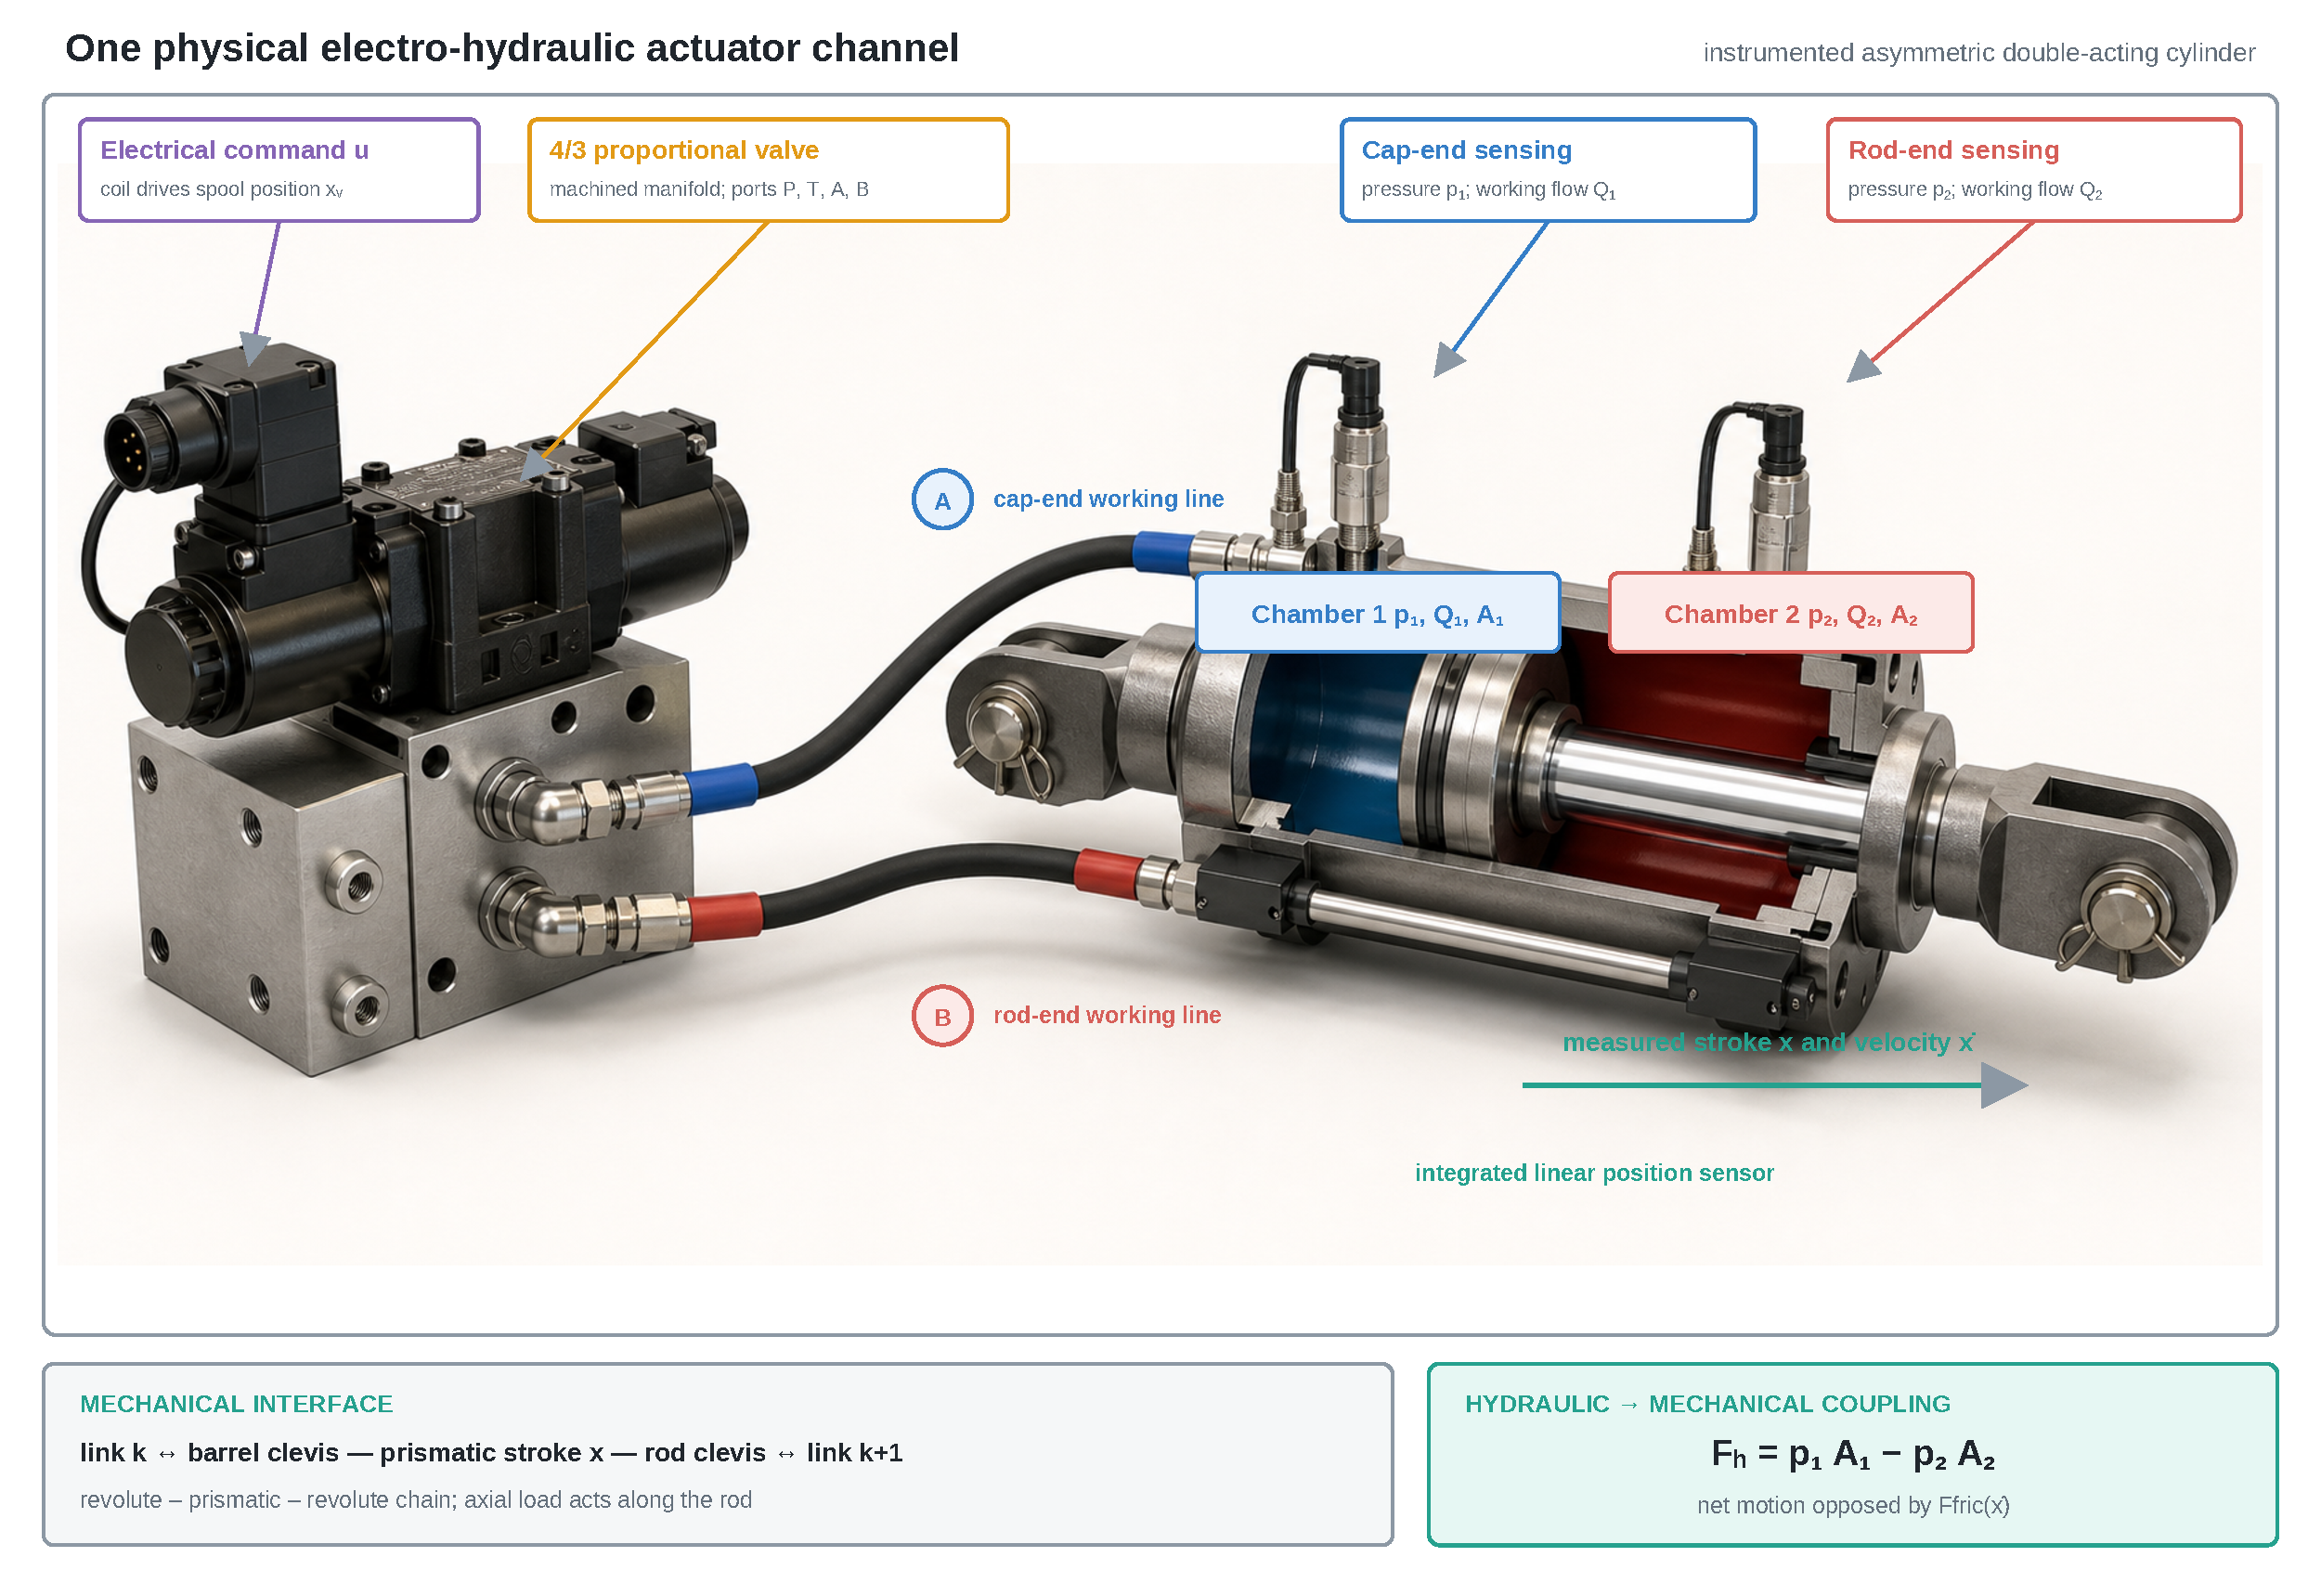
\includegraphics[width=\textwidth]{images/fme500_actuator_channel_detailed}
  \caption{One electro-hydraulic actuator channel. Top:
  the mechanical interface, in which barrel and rod connect to the adjacent
  links through a revolute--prismatic--revolute chain whose prismatic
  coordinate is the stroke $x$. Bottom: the hydraulic interface, an asymmetric
  double-acting cylinder with chamber pressures and flows routed to ports A and
  B of the proportional valve.}
  \label{fig:sys:actuator-channel}
\end{figure}

Figure~\ref{fig:sys:schematic} shows the assembled plant at system
level. The hydraulic side is deliberately physical rather
than phenomenological. Supply comes from a fixed-displacement pump
driven at variable speed ($Q_p = D_p\,\omega$), buffered by a
gas-charged accumulator (polytropic gas model) and protected by a
pressure-relief valve, so supply pressure is a dynamic quantity that
sags under simultaneous demand and clips under load spikes. Each of the four
actuators is a 4/3 proportional directional valve driving an
asymmetric double-acting cylinder.
Figure~\ref{fig:sys:actuator-channel} details one such channel, from
the rigid-body assembly of barrel and rod through the
mechanical--hydraulic coupling interface down to the valve, the
chambers, and the measured feedback signals. The chamber pressures
follow the continuity equations
%
\begin{equation}
  \label{eq:sys:continuity}
  \dot{p}_1 = \frac{E_{\mathrm{eff}}}{V_1(x)}
    \bigl( Q_1 - A_1 \dot{x} - C_{\mathrm{leak}}(p_1 - p_2) \bigr),
  \qquad
  \dot{p}_2 = \frac{E_{\mathrm{eff}}}{V_2(x)}
    \bigl( -Q_2 + A_2 \dot{x} + C_{\mathrm{leak}}(p_1 - p_2) \bigr),
\end{equation}
%
with stroke-dependent chamber volumes $V_{1,2}(x)$ that include the
line dead volumes, piston areas $A_1 \neq A_2$, and laminar internal
leakage $C_{\mathrm{leak}}$. The effective bulk modulus accounts for
entrained air through
%
\begin{equation}
  \label{eq:sys:bulk}
  E_{\mathrm{eff}}(p) =
  \left( \frac{1}{E_f} + \frac{\alpha}{p} \right)^{-1},
\end{equation}
%
so fluid stiffness itself is pressure dependent, weakest where precise low-pressure positioning is attempted. Valve flow follows the
orifice law of Chapter~\ref{chap:fundamentals}
(Section~\ref{sec:fund:actuation-chain}), and the spool is not an instantaneous
gain but a first-order lag, $\dot{x}_v = (u - x_v)/\tau_v$, so command
transients are bandwidth limited. The net piston force
$F_h = p_1 A_1 - p_2 A_2 - F_{\mathrm{fric}}(\dot{x})$ feeds back into
the mechanism through the virtual-work mapping of
Section~\ref{sec:sys:kinematics}, closing the bidirectional coupling:
mechanical loads shape pressure transients, and pressure transients
shape motion. Because cylinder-induced stiffness is high while
rigid-body motion is slow, the coupled equations are stiff, and the
model runs under a variable-step implicit solver. This stiffness is the
computational reason the Simscape plant cannot serve as an RL training
environment (Section~\ref{sec:fund:sim-data-source}).

\subsection{Validated Scope of the Model}
\label{sec:sys:simscape-validation}

A plant model intended as a data generator must be trusted for its
\emph{dynamics}, not just its geometry. The validation strategy in the
modeling study was control-based: a fixed integral backstepping
controller at $\unit[0.01]{s}$ was applied as a standardized excitation
instrument, and the emergent behavior of the closed loop was examined
as the physical parameters varied. The headline experiment sweeps the
effective bulk modulus over $\beta \in \{0.5, 1.0, 1.5, 2.0\}\,
\mathrm{GPa}$, the physically meaningful range from strongly aerated to
very stiff fluid, with all controller gains held constant. Actuation delay behaves as hydraulic intuition demands. The valve-to-joint
delay of the heavy slew axis falls from about $\unit[0.85]{s}$ at $\unit[0.5]{GPa}$ to $\unit[0.65]{s}$ at
$\unit[2.0]{GPa}$, the system-level delay index from roughly
$\unit[0.45]{s}$ to $\unit[0.35]{s}$, and the improvement saturates
beyond $\unit[1.5]{GPa}$, where mechanical inertia rather than fluid
compliance limits the response. Task-space tracking error falls
monotonically with stiffer fluid, by about 11\,\% over the sweep. The
model, in other words, reproduces the ``stiff yet oscillatory''
character of real hydraulic machinery and responds to parameter changes
in the physically expected direction, which is the property that Chapter~\ref{chap:data} exploits when it randomizes these same
parameters to generate plant families.



Three limitations are carried forward honestly. The model is a single
machine: manufacturing spread enters only through the deliberate
parameter randomization of Chapter~\ref{chap:data}, not through
measured variation. Thermal dynamics are not modeled. Temperature
effects are represented indirectly through the parameters they act on
(bulk modulus, friction). And the logged rod-force channel failed a
piston-area consistency audit on the current export
(Section~\ref{sec:models:rom}), so force is treated as unreliable
supervision throughout the thesis.

\section{IsaacLab Environment}
\label{sec:sys:isaaclab}

Policy training, adaptation-data collection, and every closed-loop
result in this thesis run in IsaacLab~\cite{mittal2023orbit} on the
GPU-parallel PhysX engine. The same CAD-derived mechanism enters here as
a USD articulation: the Unimog carrier with wheels, the five arm links,
and the four cylinders represented as prismatic actuator joints, with
self-collisions enabled and the solver configured for the long-chain
mechanism. Figure~\ref{fig:sys:unimog} renders that articulation
directly from the asset the environment loads. The complete machine is shown once, because the arm-only views of
Section~\ref{sec:sys:platform} miss the geometry that defines the task. The
boom is mounted on the front of a road-going carrier and reaches out to one
side. The cutter therefore works several metres from the vehicle carrying it,
while that vehicle keeps driving. Every
lever arm, every reaction force on the chassis, and the entire reason
the vehicle's motion must be treated as part of the plant follow from
this arrangement.

\begin{figure}[tb]
  \centering
  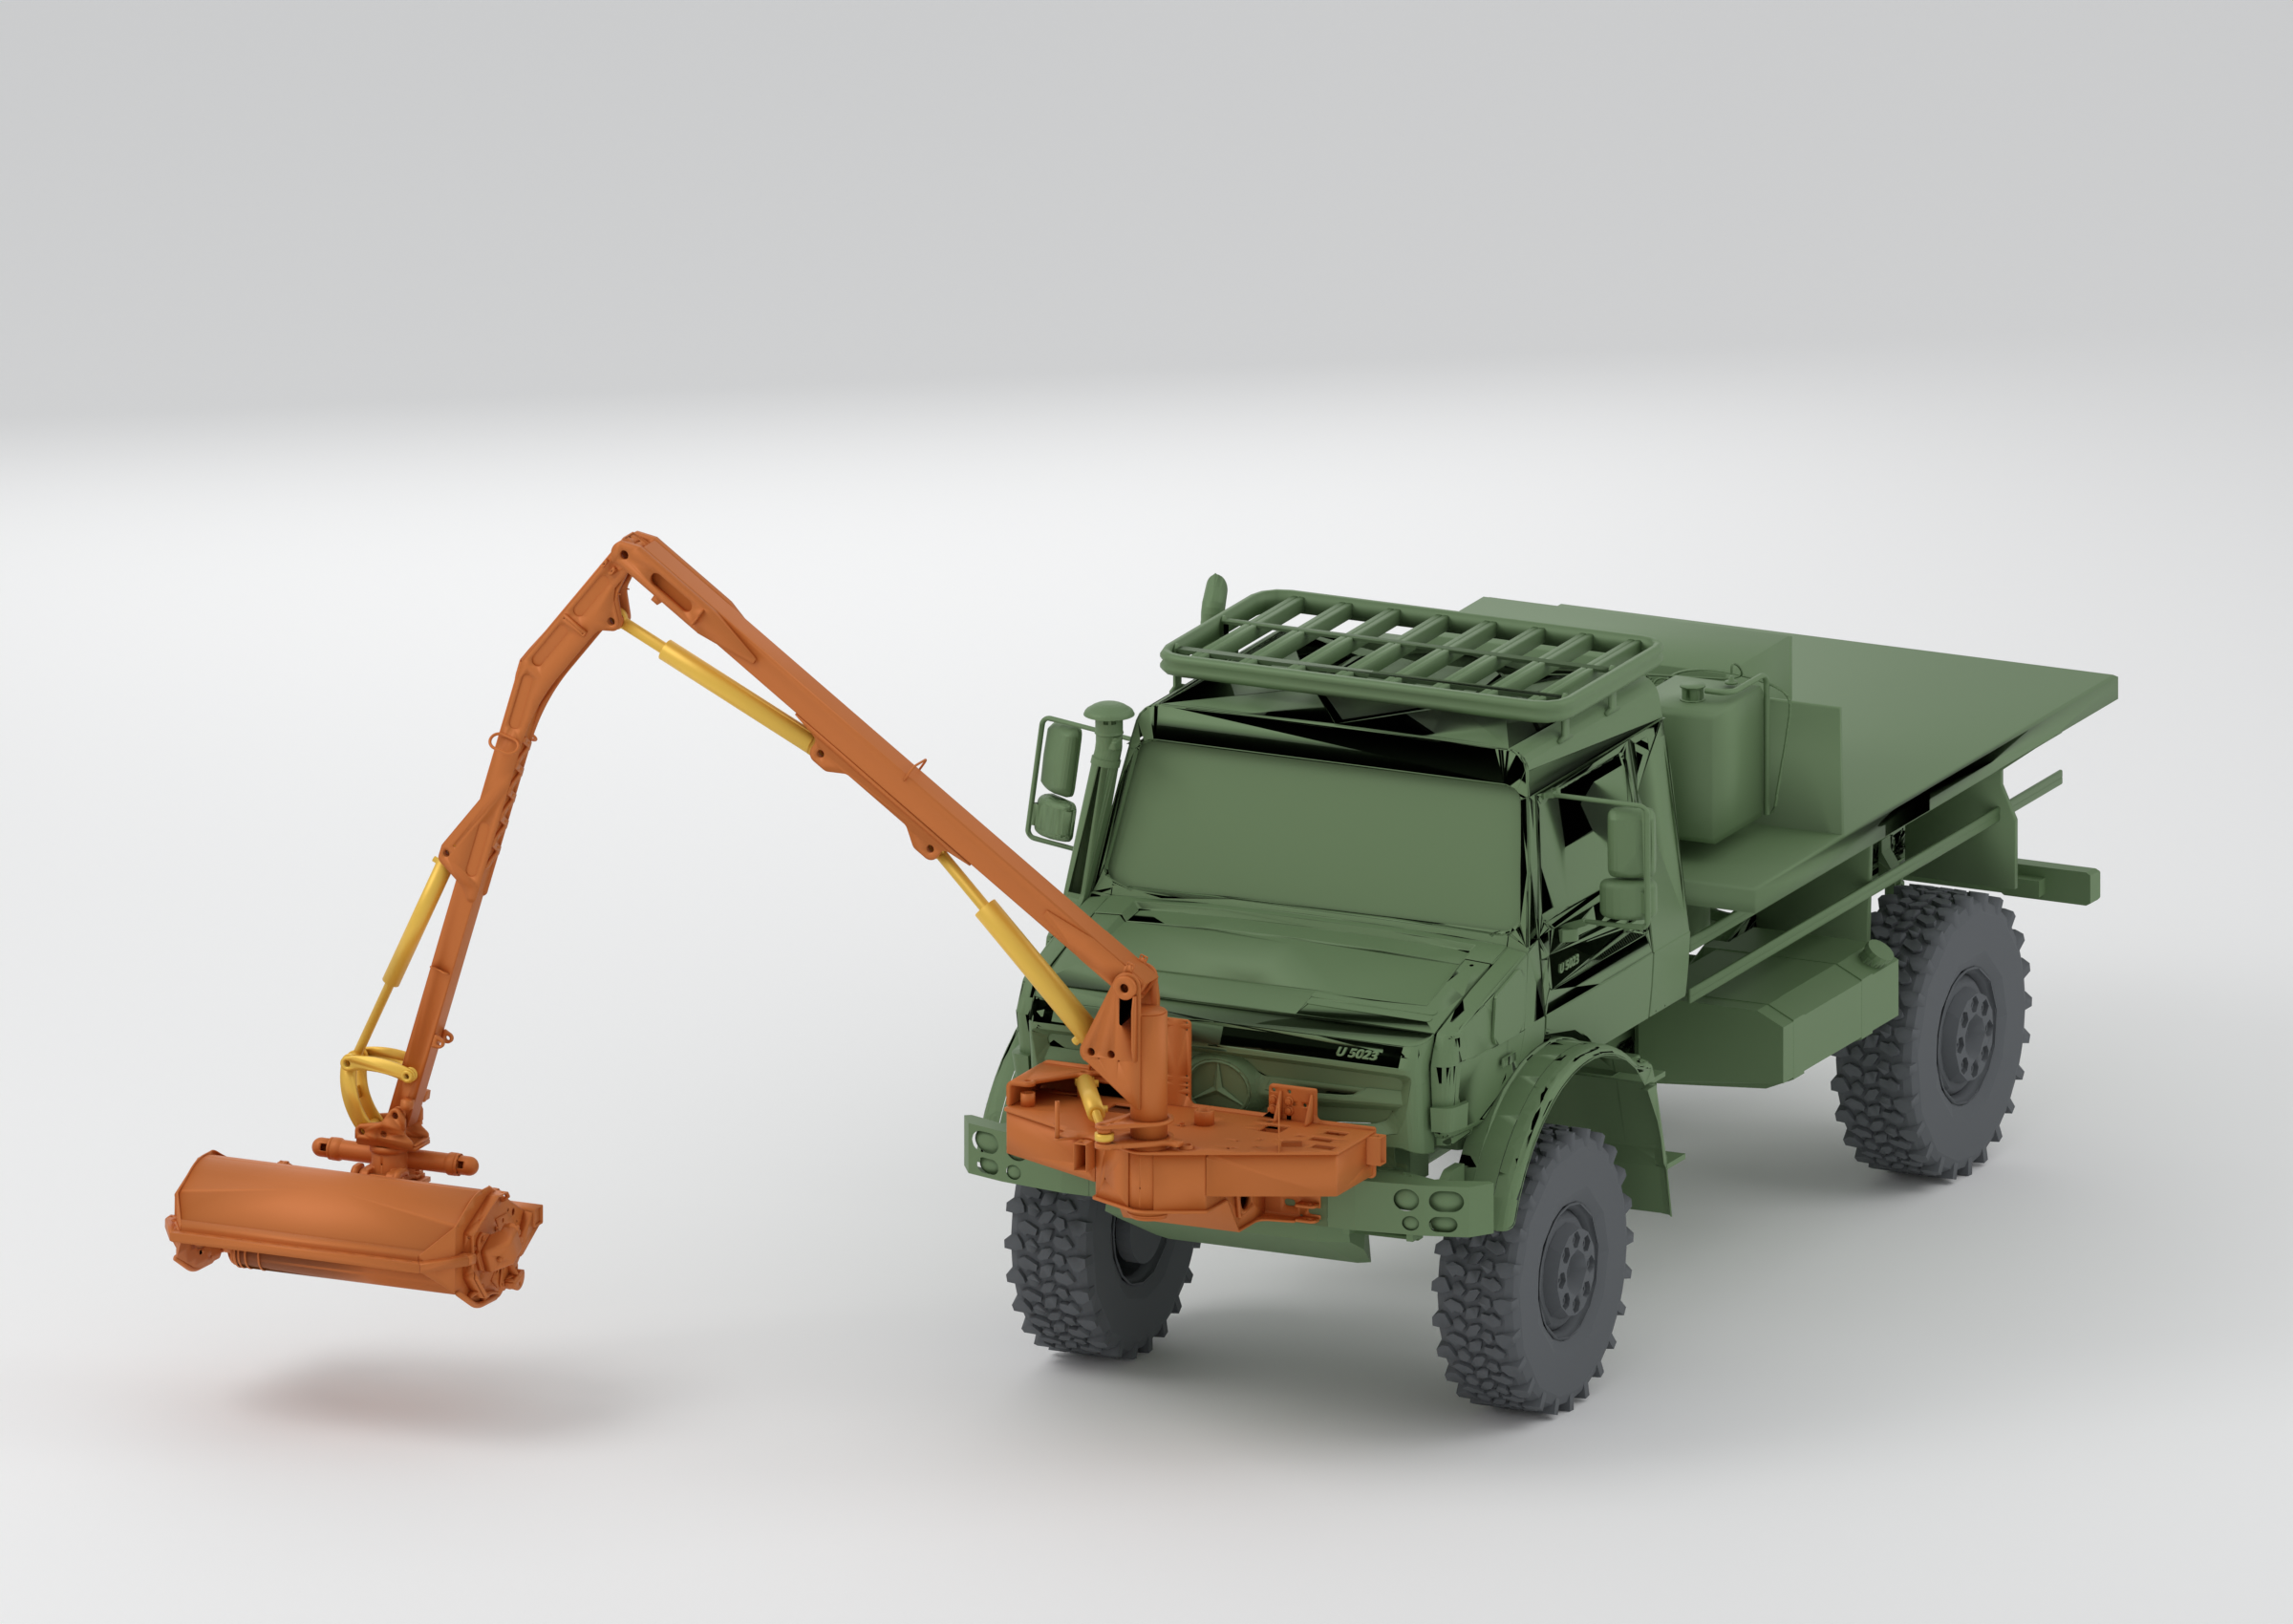
\includegraphics[width=.62\textwidth]{images/unimog_mulag_iso}
  \caption{The complete simulated machine, rendered from the USD
  articulation that the IsaacLab environment loads: the Unimog carrier with the
  FME~500 boom on its front frame and the flail head deployed to the side.
  Cylinders are highlighted in orange. The hydraulics are not present here and
  enter only through the learned actuator models.}
  \label{fig:sys:unimog}
\end{figure}

The full hydraulic model does not run inside these environments, for the
computational reasons of Section~\ref{sec:fund:sim-data-source}. Its
behavior enters only through the learned actuator representations
sitting between the controller and the PhysX cylinder targets.

\subsection{Simulation and Control Rates}
\label{sec:sys:timing}

Four different clocks run in this system, and reporting any one of them
as ``the control frequency'' misstates the interface. They are listed in
Table~\ref{tab:sys:rates}. The physics step is $\unit[1/120]{s}$ with a
control decimation of two, so the policy observes and acts at
$\unit[60]{Hz}$ ($\unit[16.7]{ms}$). The learned actuator models keep
the native $\unit[0.05]{s}$ transition they were identified on: three
consecutive control steps make one model tick, so a learned-model
prediction is issued once every three policy steps and the resulting
motion is distributed over the intervening PhysX updates as held
increments. Nothing is interpolated onto the model grid, and the
learning samples of Chapter~\ref{chap:data} use exactly those
$\unit[50]{ms}$ transitions at control indices $0, 3, 6, \dots$. A
model asked to predict across a mismatched interval is a silent
$\unit[33]{\%}$ error in the quantity it is supposed to supply. The AAM
of Chapter~\ref{chap:models} updates on the same $\unit[50]{ms}$ model
grid from a causal history window, and logging runs at the control rate.

\begin{table}[tb]
  \centering
  \caption{The four rates of the simulated system. They are reported
  separately throughout the thesis; ``the control frequency'' is not a
  well-defined quantity here.}
  \label{tab:sys:rates}
  \small
  \begin{tabular}{lll}
    \toprule
    Layer & Step & Rate \\
    \midrule
    PhysX physics                & $\unit[1/120]{s}$   & $\unit[120]{Hz}$ \\
    Policy / control (decimation 2) & $\unit[1/60]{s}$ & $\unit[60]{Hz}$ \\
    Learned actuator model (3 control steps) & $\unit[0.05]{s}$ & $\unit[20]{Hz}$ \\
    AAM latent update            & $\unit[0.05]{s}$    & $\unit[20]{Hz}$ \\
    \bottomrule
  \end{tabular}
\end{table}

\subsection{Environment Configuration Details}

Three environment details cost real debugging time and are recorded
here so they need not be rediscovered. First, the articulation root of
the arm sits about $\unit[1.11]{m}$ above the wheel contact plane, so
the vehicle must spawn with its root at $z = \unit[1.26]{m}$. Spawning
at ground height buries the truck to its axles and silently changes
every contact force. Second, cylinder actuation uses PhysX position
targets, and the target must be integrated in \emph{reference} space,
accumulating commanded increments, rather than re-anchored each step to
the measured position: re-anchoring lets gravity sag wash out every
commanded increment, removing the policy's authority entirely. Third,
the vehicle's forward motion is \emph{scripted} rather than driven
through the wheels: the chassis is advanced kinematically along the road
at the commanded speed and its lateral position and heading are held by
a planar fixture. This is not a convenience. The authored tyres and
suspension of this asset do not produce usable traction in PhysX, and
leaving the chassis free turns arm reaction forces into slow drift and
sway that contaminate every task-space error. The residual sway the
fixture has to remove is itself measured and gated
(Section~\ref{sec:sys:evaluation-criteria}) rather than assumed to be
zero.

\section{The Verge-Following Task}
\label{sec:sys:task}

\subsection{Task Definition}

The primary task of this thesis, and the one every reported control
result is measured on, is verge following with the vehicle in motion.
The truck drives along the road at a constant speed of $\unit[4]{km/h}$
in the development configuration, reduced to $\unit[2]{km/h}$ for the
final \ppoROM{} task of Section~\ref{sec:ctrl:ppo-rom}, where the strip
is lengthened to $\unit[26]{m}$. Meanwhile the
four-cylinder arm reaches over the embankment and holds the cutter on
the verge centre line: near the target cut height, in ground contact,
head down, and inside the mechanical travel limits. Tracking the line is
the objective. The terrain is a \emph{disturbance} that makes tracking
nontrivial, not an obstacle course to be negotiated, and its height
profile is randomized per environment so that no policy can memorize one
ground surface.

Reference paths are drawn from eleven families ( \texttt{straight},
\texttt{lateral\_sine}, \texttt{s\_curve}, \texttt{random\_spline},
\texttt{offset\_return}, \texttt{boom\_sweep}, \texttt{lateral\_chirp},
\texttt{double\_s\_curve}, \texttt{lane\_change\_hold},
\texttt{gaussian\_slalom}, and \texttt{fourier\_meander}),
which span
a range of lateral demand rather than a single nominal line. Because
aggregate scores can hide one impossible family behind ten easy ones,
the acceptance criteria of
Section~\ref{sec:sys:evaluation-criteria} are evaluated at the
\emph{worst} family and the \emph{worst} terrain mesh rather than pooled.

\subsection{Task Feasibility and Plant Capability}
\label{sec:sys:capability}

One finding governs the design of everything above, and it is stated
here because it is a property of the plant rather than of any
controller. The action contract commits at most $\unit[4]{mm}$ of
cylinder travel per step on cylinders~1--3
(Chapter~\ref{chap:control}), and over the interval across which that
increment is committed this bounds the lateral cutter rate at
%
\begin{equation}
  \label{eq:sys:rate-ceiling}
  v_{\mathrm{lat}}^{\max} \approx \unit[0.200]{m/s}.
\end{equation}
%
\todo{confirm the exact interval used in the maintained figure: the
$\unit[0.200]{m/s}$ ceiling is quoted as $\unit[4]{mm}/\unit[20]{ms}$,
while the environment's control step is $\unit[1/60]{s} =
\unit[16.7]{ms}$ (Table~\ref{tab:sys:rates}), which would give
$\unit[0.24]{m/s}$. Fix one and propagate.}
At the settings used before this was measured, nine of the
eleven path families demanded more lateral rate than that, one of them
(\texttt{boom\_sweep}) by a factor of $3.7$. Tracking error then
accumulates \emph{by construction}: no reward shaping, critic change, or
policy-optimization fix can recover a target the actuator cannot reach,
and indeed the privileged DLS teacher failed on those families too,
which is the diagnostic that identified the problem. The terrain and
path parameters are therefore now \emph{derived} from
\eqref{eq:sys:rate-ceiling} rather than chosen independently of it, and
a preflight check asserts the resulting feasibility before any training
run is allowed to start.

The methodological rule generalizes beyond this machine and is applied
throughout the thesis: before attributing a tracking failure to the
learning algorithm, measure whether the commanded reference is inside
the actuator's authority. A task outside the plant's capability produces the symptoms of a badly tuned policy.

\subsection{Parked Diagnostic Workflow}
\label{sec:sys:parked}

A second, older workflow is retained and must not be confused with the
task above. With the vehicle held stationary, the cutter tracks
scripted line, arc, sine, circle, and square references in free space.
This is a \emph{diagnostic} instrument for qualifying the plant and the actuator models
(step response, per-axis authority, out-and-back return error, and
Jacobian conditioning), and it is how several of the
cylinder-level checks in this thesis are performed. It is not a fourth
control stack, it is not part of the final comparison, and its numbers
are never pooled with the moving-verge statistics. Where a parked result
is reported, it is labelled as a separate diagnostic experiment.

\section{Control Architecture}
\label{sec:sys:architecture}

\begin{figure}[tb]
  \centering
  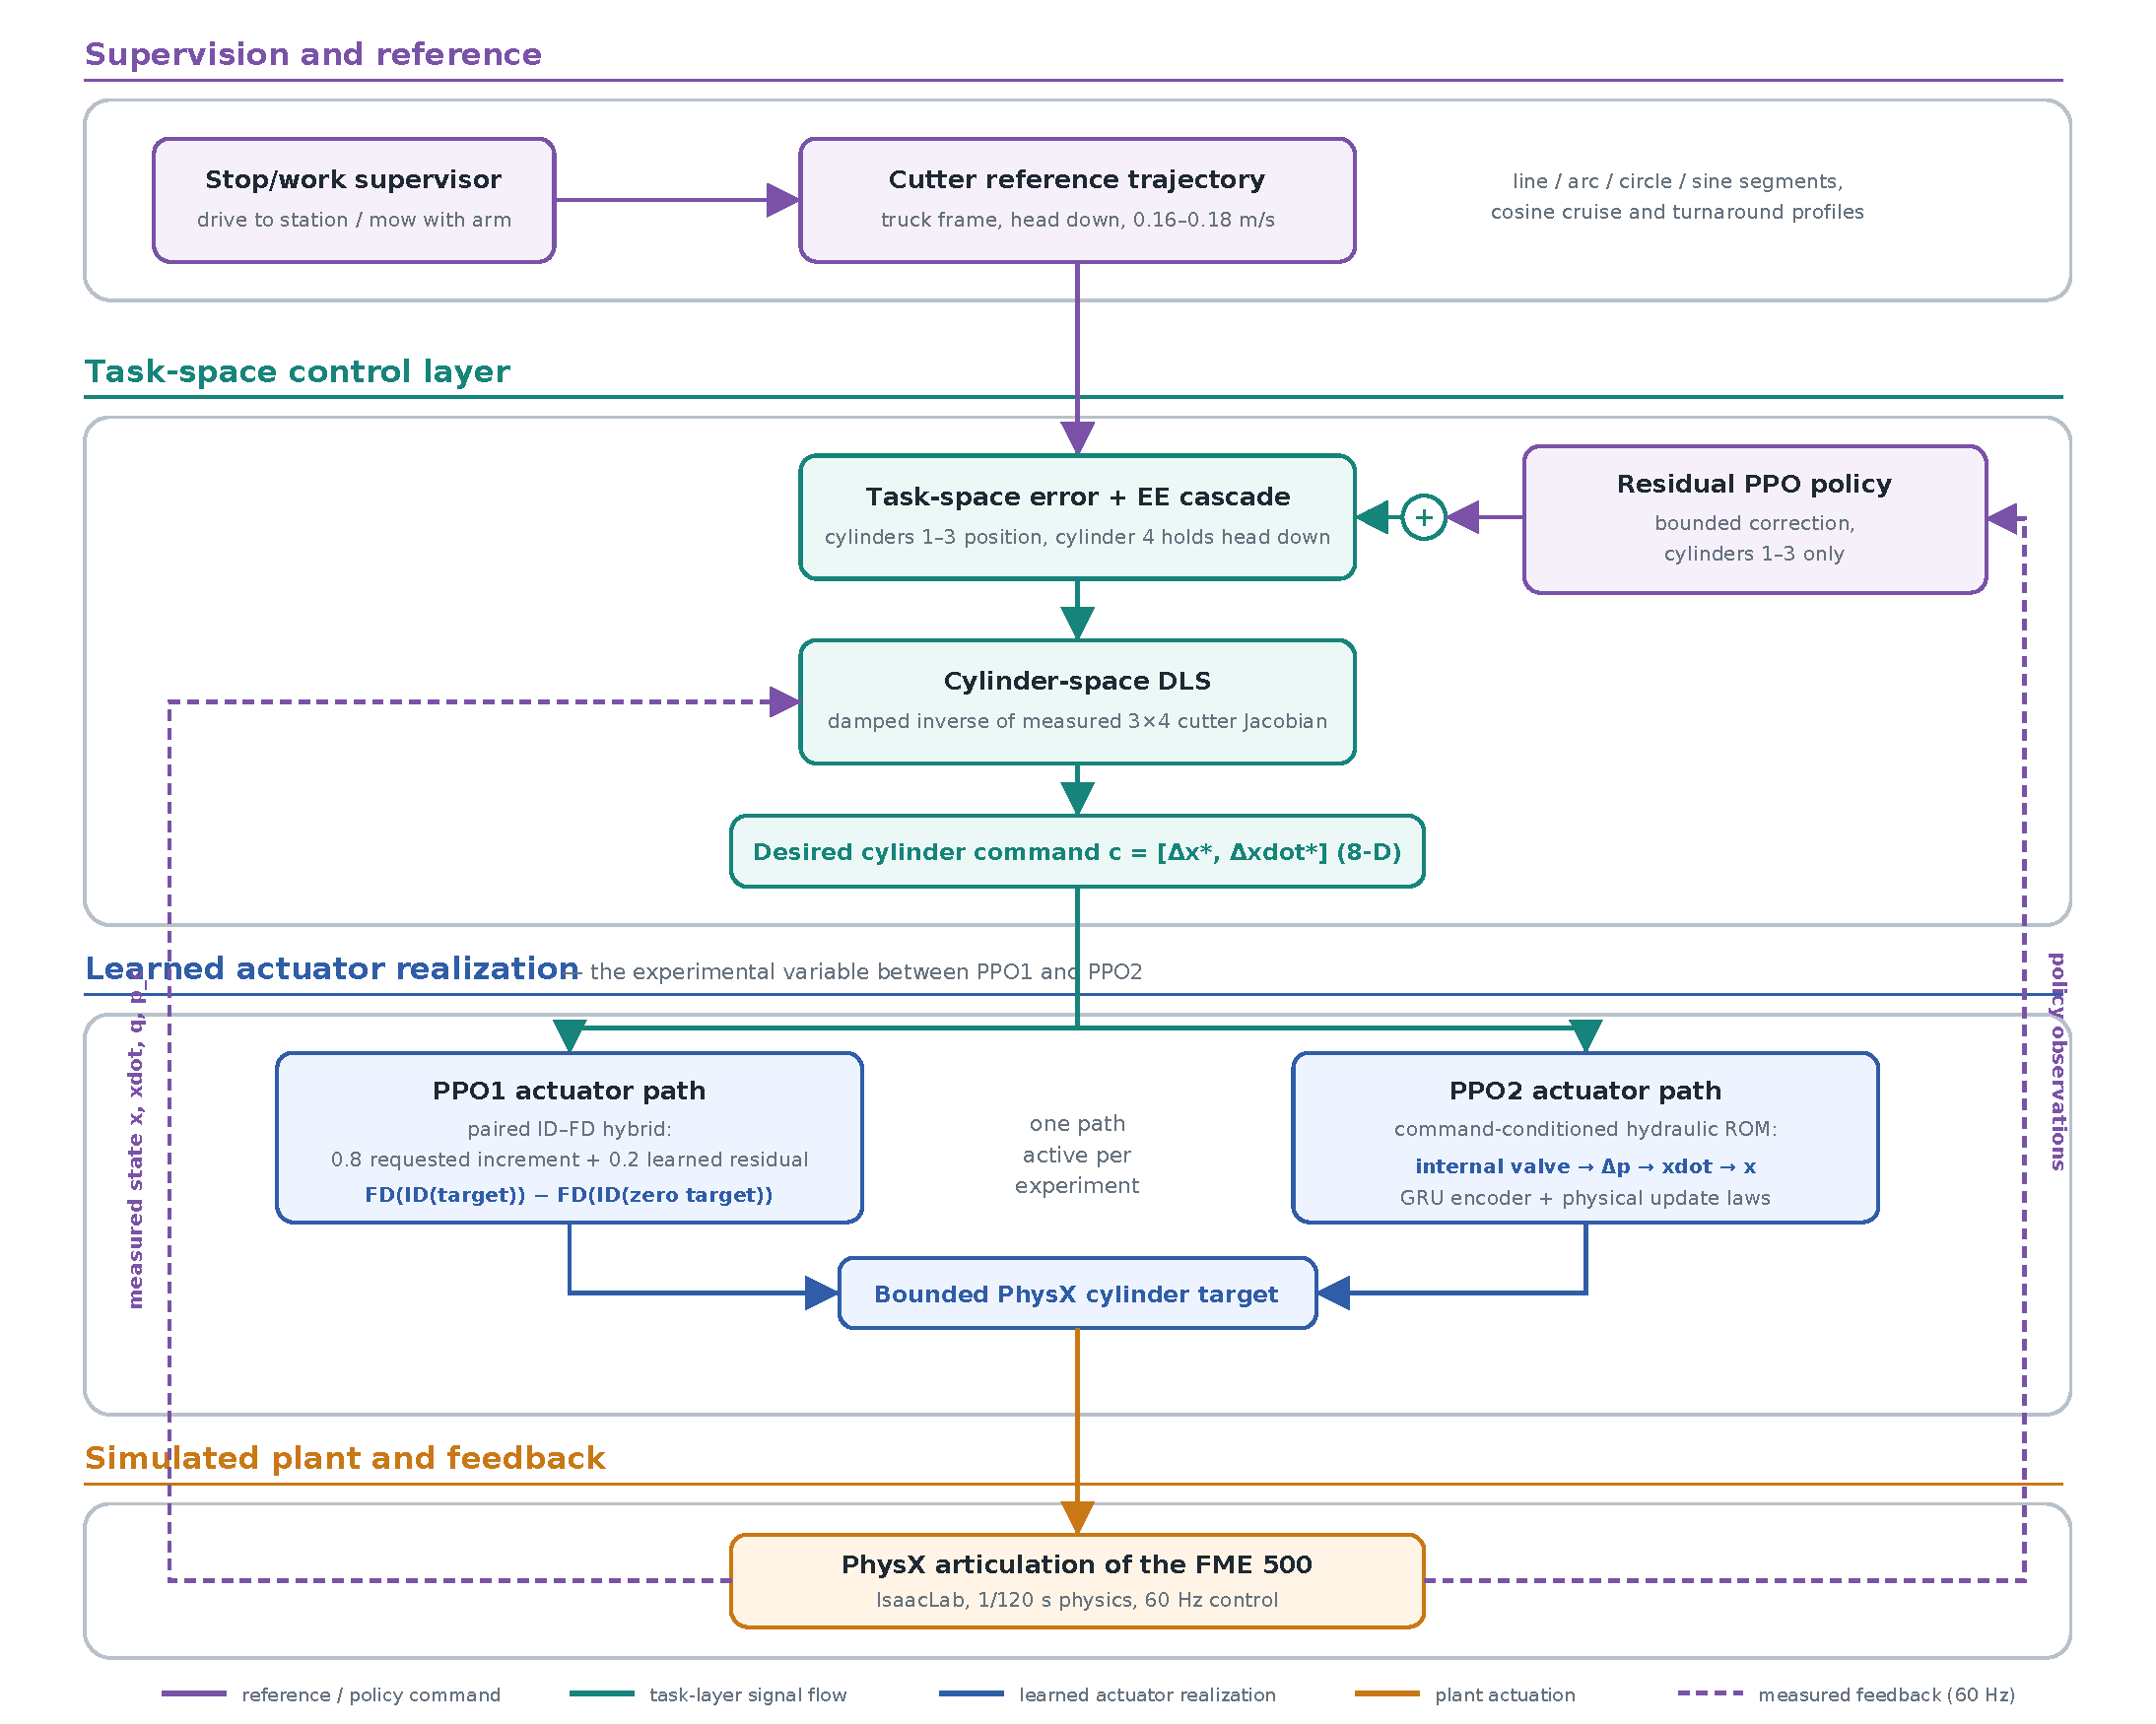
\includegraphics[width=.95\textwidth]{images/fme500_control_architecture}
  \caption{Control architecture used in all experiments,
  organized by layer. The vehicle layer advances the chassis and the reference
  generator supplies the verge centre line. The policy emits four normalized
  cylinder commands, which pass through the action contract to the learned
  actuator layer. Only that actuator layer differs between the three stacks.
  The DLS controller sits outside the deployed loop: it is the teacher and the
  identification controller, not a runtime layer.}
  \label{fig:sys:architecture}
\end{figure}

Figure~\ref{fig:sys:architecture} assembles the pieces. The vehicle layer
advances the chassis at the scripted speed of Section~\ref{sec:sys:task} and is
not under policy control. The reference generator supplies the verge centre
line and the target cut height.

The policy is the entire task layer. It reads normalized observations of the
terrain, the tracking errors and the cylinder and actuator state, and emits
four desired cylinder-motion commands. It is \emph{not} a residual: no nominal
command is added at runtime and no baseline controller sits underneath it. What
keeps its commands inside the learned actuator's validated envelope is the
action contract. The damped least-squares inverse appears twice in this thesis,
as the privileged teacher and as the controller that drove the identification
runs of Chapter~\ref{chap:data}, but never inside the deployed loop.
Chapter~\ref{chap:control} specifies the observation, the action contract and
the teacher in full.

Below the task layer sits the experimental variable of the whole thesis: the
actuator path that realizes the desired cylinder command. \ppoROM{} realizes it
with the command-conditioned reduced-order model, \ppoIDFD{} with the frozen
inverse and strict forward pair, and \ppoIDAAMFD{} with that same pair plus a
small bounded adapter conditioned on the inferred latent $\latenthat$. All
three end in the same bounded PhysX cylinder position target, and the measured
state closes the loop at the rates of Table~\ref{tab:sys:rates}.

\section{Problem Formulation}
\label{sec:sys:problem}

With the system fixed, the control problem can be stated compactly.
The vehicle advances at constant speed, so the reference is not a free
three-dimensional trajectory. It is a verge centre line
$y_{\mathrm{ref}}(t)$ and a target cut height $h_{\mathrm{ref}}$, both
expressed in the truck frame and drawn from the eleven path families of
Section~\ref{sec:sys:task}. Writing $\bm{p}_c(t)$ for the measured
cutter-tip position and $g(\cdot)$ for the terrain height beneath it,
the two scored errors are
%
\begin{equation}
  \label{eq:sys:error}
  e_{\mathrm{lat}}(t) = p_{c,y}(t) - y_{\mathrm{ref}}(t),
  \qquad
  e_{\mathrm{cut}}(t)
    = \bigl(p_{c,z}(t) - g(\bm{p}_c(t))\bigr) - h_{\mathrm{ref}} .
\end{equation}
%
The \emph{tracking objective} is to keep $|e_{\mathrm{lat}}|$ and
$|e_{\mathrm{cut}}|$ small in mean and in the tail over complete
episodes, on every path family and on unseen terrain, while the cutter
stays in ground contact, the head stays down, and the motion remains
smooth enough not to damage the machine. The \emph{model objective},
developed in Chapter~\ref{chap:models}, is that each learned actuator
representation predict the cylinder response to its commands accurately
over one step and over recursive rollouts, with demonstrated input
authority. The \emph{robustness objective} asks that this performance
persist across the randomized plant family $\{\mathcal{P}(\factorvec)\}$
of Chapter~\ref{chap:data}. The \emph{adaptation objective} asks that
the stack conditioned on the inferred latent $\latenthat$ recover
performance on held-out factor configurations, further than the
non-adaptive stack and approaching the privileged true-latent oracle,
without degrading the nominal domain and without violating any
acceptance gate.

All objectives are subject to the same constraint set: cylinder
extensions within the ranges of Table~\ref{tab:sys:cylinders} with a
positive travel margin retained, per-step commanded increments and
target leads bounded by the action contract of
Chapter~\ref{chap:control}, valve or adapter outputs within the per-axis
limits stored in the learned checkpoints, and the head held down
throughout.

No single ingredient makes this problem hard. The difficulty is their
combination, and each chapter so far has contributed one piece: the actuator chain is nonlinear and drifting
(Chapter~\ref{chap:fundamentals}), only three task directions are
controllable and the mapping into them varies with configuration
(Section~\ref{sec:sys:kinematics}), the true actuator state is not
observable at runtime (Section~\ref{sec:sys:actuation}), the reference
sits close to the plant's own rate ceiling
(Section~\ref{sec:sys:capability}), the ground is a randomized
disturbance rather than a known surface, and the high-fidelity plant
that knows the hydraulic answers is too slow to train against
(Section~\ref{sec:sys:simscape}).

\section{Evaluation Criteria at System Level}
\label{sec:sys:evaluation-criteria}

The thesis judges controllers and models by fixed, pre-registered
gates rather than by single aggregate scores, and it separates the two levels: a controller metric can hide model weakness behind
policy compensation (Section~\ref{sec:fund:rl-residual}), so model
metrics are always reported alongside.

\subsection{The Eight-Gate Task Contract}

At the \emph{system level}, acceptance is an eight-gate contract, listed
in Table~\ref{tab:sys:gates}. Each gate matches something an operator would notice. It cuts at the right
height, follows the line, stays on the ground, keeps the head down, and does not slam into
the terrain, it does not shake itself apart, it does not drive into its
own travel limits, and its episodes complete.

\begin{table}[tb]
  \centering
  \caption{The eight acceptance gates. Every gate is evaluated on at
  least three distinct terrain meshes and reported at its \emph{worst}
  mesh, and the two tracking-critical gates additionally at the worst
  path family. Final claims use six held-out meshes.}
  \label{tab:sys:gates}
  \small
  \begin{tabular}{llll}
    \toprule
    Gate & Metric & Threshold & Aggregation \\
    \midrule
    Cut height        & mean $|e_{\mathrm{cut}}|$
                      & $\leq \unit[0.040]{m}$ & worst mesh \\
    Lateral tracking  & mean $|e_{\mathrm{lat}}|$
                      & $\leq \unit[0.300]{m}$ & worst mesh, worst family \\
    Ground contact    & contact fraction
                      & $\geq 0.700$ & worst mesh, worst family \\
    Head alignment    & p01 head-down alignment
                      & $\geq 0.900$ & worst mesh \\
    Hard impacts      & hard-impact step fraction
                      & $\leq 0.100$ & worst mesh \\
    Tool acceleration & p95 cutter acceleration
                      & $\leq \unit[120]{m/s^2}$ & worst mesh \\
    Cylinder headroom & minimum travel margin
                      & $\geq \unit[0.005]{m}$ & worst mesh \\
    Safety terminations & termination rate
                      & $\leq 0.080$ & worst mesh \\
    \bottomrule
  \end{tabular}
\end{table}

Three rules about \emph{how} these gates are used matter more than the
thresholds themselves, and each of them was adopted after a measured
failure of the previous practice.

\paragraph{Multi-Mesh Evaluation}
An earlier contract scored every result on a single pinned terrain seed.
When the mesh was finally varied, both the headline pass and the headline failure moved a long way:
minimum head alignment ranged
$0.9027$ to $0.9698$ across three meshes, and a checkpoint that
``passed'' by $0.0007$ on the pinned mesh failed on the others. A gate
that flips with the mesh is measuring the mesh. Results here are
therefore refused unless they are measured on at least three meshes, and
reported at the worst.

\paragraph{Gating at the Optimized Resolution}
The same earlier contract read worst-of-eleven-family minima while the
optimizer maximized a pooled mean. Across ten training blocks the mean
ground contact rose from $0.817$ to $0.870$ while the worst-family
contact never left the $0.66$--$0.75$ band: nothing was optimizing what
acceptance measured.

\paragraph{Measurement-Anchored Thresholds}
A gate that nothing can pass carries no information, and several were found in that state. The tool-acceleration limit stood at
$\unit[80]{m/s^2}$ while the environment alone, with the arm commanded
to zero, measures a p95 of $\unit[100.06]{m/s^2}$. It was re-derived to
$\unit[120]{m/s^2}$, $1.2\times$ the measured floor. The ground-contact
and hard-impact thresholds were likewise anchored just outside what the
privileged DLS teacher itself achieves, so that they separate a working
controller from a non-working one rather than separating the teacher
from perfection. Every threshold in
Table~\ref{tab:sys:gates} is therefore accompanied in the source by the
measurement that fixes it, and every reported result carries its signed
margin rather than a bare pass or fail, so that a pass by $0.0007$
cannot masquerade as a comfortable one.

\subsection{Cylinder- and Model-Level Criteria}

At the \emph{cylinder level}, the parked diagnostic workflow of
Section~\ref{sec:sys:parked} supplies step gates: clean response to
fresh $\pm\unit[10]{mm}$ commands on every axis, small terminal error on
large ($\unit[80]{mm}$) coordinated motions, and low out-and-back return
error, all without command saturation. Model-level criteria
(one-step and rollout accuracy, input-ablation authority, and Jacobian
conditioning) were introduced with the models in
Chapter~\ref{chap:models}. Chapter~\ref{chap:evaluation} instantiates
all three families of criteria in the full experimental matrix, and
treats the eight-gate contract as the minimum acceptance criterion
rather than as a substitute for reporting full distributions.

The system is now specified. The next chapter turns to the data the learned
models are built from.

%%%%%%%%%%%%%%%%%%%%%%%%%%%%%%%%%%%%%%%%%%%%%%%%%%%%%%%%%%%%
%% Chapter 4 — Data Generation and Preparation (10–16 pages)
%% Purpose: explain how the Simscape datasets were designed to
%% contain realistic operation, causal actuator excitation, and
%% variation required for robust and adaptive learning.
%%%%%%%%%%%%%%%%%%%%%%%%%%%%%%%%%%%%%%%%%%%%%%%%%%%%%%%%%%%%
\chapter{Data Generation and Preparation}
\label{chap:data}

Chapter~\ref{chap:system} fixed the plant. It did not fix how its two
simulated representations meet. The Simscape model knows the hydraulics but is
far too slow to train a policy against, and the IsaacLab articulation is fast
but has no hydraulics at all. Everything the learned models of
Chapter~\ref{chap:models} can say about the actuator has to travel from the
first world to the second inside a dataset. This chapter describes how those
datasets were designed, collected, audited and prepared.

The datasets come from two different sources, and keeping their provenance
straight is a precondition for reading the results honestly
(Table~\ref{tab:sys:provenance}).

\emph{Historical Simscape provenance.} Two Simscape campaigns identified
the frozen actuator models that this thesis carries forward as
comparison components: the command-conditioned reduced-order model and
the inverse/strict-forward pair. The first campaign drives the arm with
a closed-loop controller and produces the realistic operating
distribution the inverse and reduced-order models learn from. The second
removes the controller entirely and applies deliberate excitation to the
valves, because the closed-loop campaign turned out to be unable, in
principle, to identify what the valve does. Section~\ref{sec:data:open-loop} sets out that diagnosis and its repair in
full, because the failure is easy to repeat and the repair is what makes the
forward model usable.

\emph{Closed-loop calibration of the ROM in IsaacLab.} The command ROM is not a pure Simscape artifact, whereas its partner in
the comparison, the ID--FD pair, \emph{is}. After
Simscape training the ROM was fine-tuned on closed-loop rollouts
collected inside IsaacLab itself, on the five plant-reachable reference
shapes, with only a small bounded correction head left trainable and the
Simscape material retained as a replay term
(Section~\ref{sec:data:rom-calibration}). It is therefore the one
actuator model in this thesis that has seen the plant it is deployed in.

\emph{The IsaacLab adaptation collection.} The system-dynamics
surrogate, the privileged factor encoder, and the Arm Adaptation Module
are not trained on Simscape data at all. They are trained on a
$118$-run collection made in IsaacLab through the deployment plant itself
(the command ROM plus PhysX), driven by the DLS controller
with dedicated PRBS excitation windows
(Section~\ref{sec:data:isaaclab}). The reason is simple: those models
exist to describe the plant the adaptive controller faces,
and that plant is the IsaacLab one. No new Simscape data was collected
for this thesis, and no earlier adaptation or system-dynamics model was
reused.

\section{Dataset Objectives and Design Requirements}
\label{sec:data:objectives}



Before any run was collected I fixed four requirements that the data had
to satisfy jointly. They are stated explicitly, because the rest
of the chapter is essentially the record of discovering that no single
collection strategy meets all four.

\begin{description}
  \item[R1: realistic operating distribution.] The learned models are
    deployed inside a tracking controller, so they must be accurate in
    the states that controller visits: coordinated multi-axis
    motion, gravity-loaded poses, moderate speeds. Data collected far
    from that distribution would be accurate where it does not matter.
  \item[R2: causal identifiability of the valve.] A forward model is
    only useful to a policy if it responds to the command. This requires
    that the valve signal in the training data carry information that the
    state history does not already carry, which is a property of the
    \emph{experiment}, not of the network~\cite{ljung1999system,
    isermann2011identification}.
  \item[R3: variation across a plant family.] Robust training and, later,
    latent adaptation both need many plants rather than one. The
    variation has to be physically meaningful, it has to demonstrably
    change the measured response, and it has to be recorded per run,
    because the privileged latent of Section~\ref{sec:models:latent} is computed from those recorded factors.
  \item[R4: clean separation.] Train, validation, and test material must
    be separable at the level of complete runs, so that no transition
    window straddles a split boundary and no run contributes to two
    splits.
\end{description}

R1 and R2 pull against each other, and that tension is the organising
idea of this chapter. A controller that produces realistic motion
computes its command from the measured state, which makes command and
state history redundant and destroys identifiability
(Section~\ref{sec:fund:identifiability}). An experiment that guarantees
identifiability has to break the feedback path, which immediately makes
the motion unrealistic. Rather than compromise on one of them, I
collected both: a closed-loop campaign that satisfies R1 and R3, and an
open-loop campaign that satisfies R2. Section~\ref{sec:data:combining}
explains how the two are used together without letting either one
dominate.

\section{Randomized Parameter Space of the Simscape Campaign}
\label{sec:data:randomization}

This section documents the randomization design of the Simscape
curriculum. Its status must be stated before its content, because the
design was drawn up under an earlier plan in which randomized
\emph{Simscape} data would be the substrate for adaptation, and that
plan is superseded. No model reported in this thesis is trained on this
curriculum. It is retained for two reasons that survive the change: it
is the provenance record of the closed-loop material the actuator models
were identified on, and the compliance-equivalence analysis of
Section~\ref{sec:data:compliance} is what taught this project which quantity is randomizable in a hydraulic chamber model, a lesson carried directly into the factor space of
Section~\ref{sec:data:isaaclab}. Readers interested only in the models
that produce results may skip to
Section~\ref{sec:data:closed-loop}.

\subsection{Sampling Design}

The closed-loop campaign draws its plants from a twelve-dimensional
parameter space using Latin hypercube sampling~\cite{mckay1979comparison},
which spreads the draws more evenly over each marginal than independent
uniform sampling would at this sample size. The twelve coordinates are
fixed once for the whole batch, before any simulation runs, so the
parameter table is reproducible and can be audited independently of the
data it produced.

The batch is organised as a curriculum rather than a single homogeneous
pool. Run~1 is the untouched nominal plant. Runs 2--251 randomize only
the hydraulics, runs 252--501 only the mechanics, and runs 502--1000
both together, giving the composition shown in
Figure~\ref{fig:data:design}(a). This structure is deliberate: it makes
it possible to attribute a later modelling failure to the hydraulic or
the mechanical axis by retraining on one block at a time, which a
uniformly mixed batch would not allow.

\begin{figure}[tb]
  \centering
  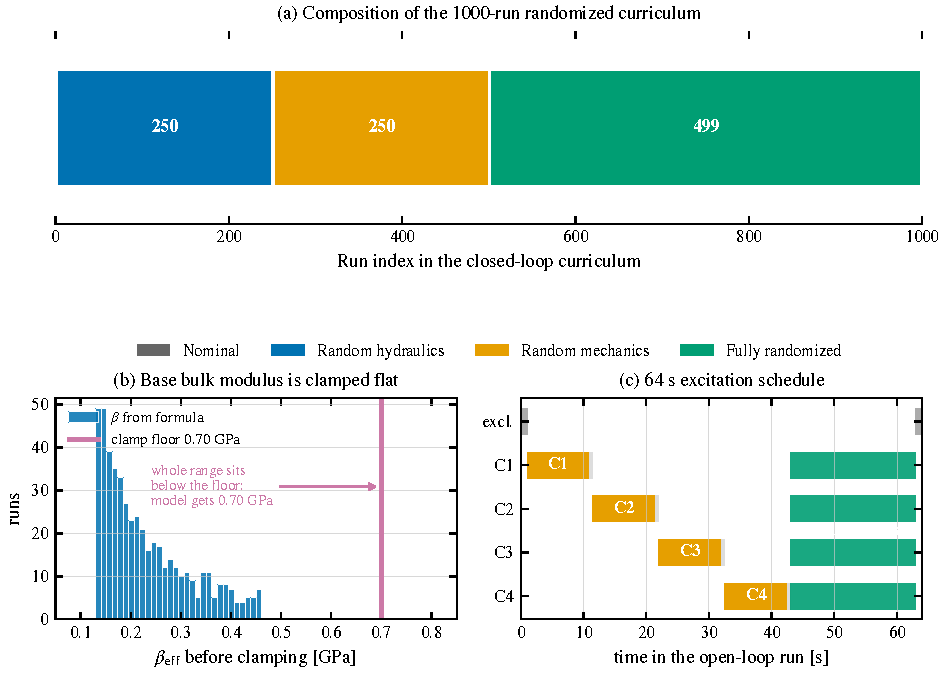
\includegraphics[width=\textwidth]{images/ch4_dataset_design}
  \caption{Design of the two collection campaigns.
  (a)~Composition of the closed-loop curriculum: one nominal run, then $250$
  hydraulics-only, $250$ mechanics-only and $499$ fully randomized draws.
  (b)~Timeline of one open-loop excitation run.}
  \label{fig:data:design}
\end{figure}

\subsection{Hydraulic Parameters}

Table~\ref{tab:data:hydraulic} lists the hydraulic axes. They were
chosen to correspond to the physical mechanisms that make one machine
differ from another in service, in the sense discussed in
Section~\ref{sec:fund:actuation-chain}: air works its way into the
fluid, spools and seals wear, and relief settings drift.



The seal-wear coordinate deserves comment because it is the one place
where a single sampled number is deliberately allowed to move several
model parameters together. A worn cylinder does not become leakier
without also becoming slower, so $w_{\mathrm{seal},i}$ scales the piston
clearance linearly, the valve leakage area with the cube of the same
factor, and the spool time constant from $\unit[8]{ms}$ to about
$\unit[13]{ms}$ at the top of the range. Sampling those three
independently would have produced physically incoherent machines, some
of them very leaky and yet perfectly fast.

\subsection{The Compressibility Axis}
\label{sec:data:compliance}

The entrained-air and dead-volume coordinates randomize the chamber dead
volume, which spans $505$ to $\unit[579]{mL}$ across the batch. This reaches
the pressure dynamics through the continuity equation
\eqref{eq:sys:continuity}, which carries the chamber volume: a larger chamber
is more compliant and slower, a smaller one stiffer and faster. The
compressibility axis therefore enters the batch as capacitance variation.

\subsection{Mechanical Parameters}

The mechanical axes, listed in Table~\ref{tab:data:mechanical}, are
applied to all fourteen rigid bodies of the mechanism: the six links,
the four cylinder barrels, and the four pistons. For each body the mass
is perturbed by up to $\pm 20\,\%$, the centre of mass by up to
$\pm 5\,\%$ of its nominal offset, and the inertia tensor together with
its products of inertia is perturbed consistently with the mass change,
so that the body remains physically realisable rather than acquiring an
inertia that its mass could not produce.



The joint stiffness and damping terms model compliance in the bearings
and linkage rather than in the fluid. They matter here because they set
how much of a pressure transient appears as boom oscillation instead of
clean motion, which is the coupling that a purely kinematic
controller cannot anticipate.

\section{Closed-Loop Data Collection}
\label{sec:data:closed-loop}

The complete closed-loop procedure is summarized in
Algorithm~\ref{alg:data:closed-loop}. Two features stand out before the prose expands on them: the parameter table is
drawn in full before any simulation runs, so the plant family is fixed
and reproducible independently of the collection, and the reference
trajectory is resampled inside every run, so no two runs share a path.

\begin{algorithm}[tb]
  \small
  \DontPrintSemicolon
  \SetKwInOut{Input}{input}\SetKwInOut{Output}{output}
  \Input{run budget $N=1000$; joint limits $\bm{q}_{\min},\bm{q}_{\max}$;
    nominal parameters $\bm{\theta}_0$}
  \Output{dataset $\mathcal{D}=\{(\text{trajectory}_i,\bm{\xi}_i)\}_{i=1}^{N}$}
  \BlankLine
  $\mathbf{L}\leftarrow\textsc{LatinHypercube}(N,12)$
    \tcp*{one design for the whole batch}
  \For{$i\leftarrow 1$ \KwTo $N$}{
    assign $i$ to a curriculum block (nominal / hydraulic / mechanical /
      full)\;
    $\bm{\xi}_i\leftarrow\textsc{DrawParameters}(\mathbf{L}_i,\text{block})$
      \tcp*{$\varepsilon_{\mathrm{air}},\varepsilon_{\mathrm{vol}},c_d,
      w_{\mathrm{seal}},p_{\mathrm{set}}$; masses, CoM, inertia,
      stiffness}
  }
  \For{$i\leftarrow 1$ \KwTo $N$}{
    inject $\bm{\xi}_i$ into the Simscape model\;
    $n_w\leftarrow\textsc{RandInt}(12,20)$;\quad
      $\bm{W}\leftarrow\textsc{LatinHypercube}(n_w,\text{JDOF})$ within
      $[\bm{q}_{\min},\bm{q}_{\max}]$\;
    assign each segment a speed class (slow / medium / fast / variable);
      \textbf{no} dwell\;
    $\bm{q}_{\mathrm{ref}}(t)\leftarrow\textsc{Interpolate}(\bm{W})$ over
      $\unit[22]{s}$\;
    simulate with \texttt{ode23t}; log on the $\unit[0.05]{s}$ grid\;
    store $(\bm{u},\bm{x},\dot{\bm{x}},\Delta\bm{p},\bm{F},\bm{q},
      \dot{\bm{q}},\bm{q}_{\mathrm{ref}},\bm{\xi}_i)$\;
    \lIf{$i \bmod 100 = 0$}{checkpoint $\mathcal{D}$ to disk}
  }
  \caption{Closed-loop curriculum generation.}
  \label{alg:data:closed-loop}
\end{algorithm}

\subsection{The Controller as a Data-Collection Instrument}

Every closed-loop run is driven by the same fixed integral-backstepping
controller, operating on all five joints at a $\unit[0.005]{s}$ rate.
Its gains are never retuned between runs. This is deliberate: the
controller is here as a standardised instrument for putting the arm
through realistic motion, not as a control contribution of this thesis,
and holding it fixed is what makes the resulting behavioural differences
attributable to the plant draw rather than to the controller.

Three details of the controller matter later. The second joint carries
the gravity load of the whole boom, so it is handled by a
proportional-integral law with velocity damping and an explicit gravity
bias rather than by the backstepping law used on the others. A barrier
term keeps the commanded configuration away from the joint limits
imported from the URDF. And the commands are saturated per axis at
$[0.95,\, 0.95,\, 0.80,\, 0.80,\, 0.90]$. That last vector matters: the first four entries are exactly the clip limits stored in the
inverse-dynamics checkpoint in Section~\ref{sec:models:id}. The ID
network inherited its output limits from the instrument that generated
its training labels, which is correct but easy to mistake for a
free design choice.

\section{Open-Loop Excitation Experiments}
\label{sec:data:open-loop}

\subsection{Limitations of the Closed-Loop Batch}

The first forward-dynamics model was trained on the closed-loop material
and scored a one-step $R^2$ near $0.999$. It was also, as
Section~\ref{sec:models:fd-identifiability} documents, almost completely
insensitive to its own valve input: zeroing that input changed the
long-horizon rollout error by a few percent. The model had learned to
continue a trajectory, not to respond to a command.

This is not a training failure and no amount of retraining on the same
material would have fixed it. In closed loop the controller computes the
command from the state, so the command is very nearly a deterministic
function of the state history that the network already
sees~\cite{ljung1999system}. The information needed to separate cause
from correlation is simply not present in the data. Recovering it
requires an experiment in which the command is generated independently
of the state, which means opening the loop.

This is not a coverage problem in disguise.
Figure~\ref{fig:data:regimes} shows that the closed-loop batch is in
fact varied in its control effort: pooled over a run, the valve spends
about a quarter of the time saturated, roughly half in the mid-authority
band, and the rest in low-command creep, so all three control regimes
are represented. The difficulty is visible in the same figure. Plotting
the valve command against the cylinder velocity it produced shows the
two riding together along a band rather than filling the plane: in a
feedback loop a fast motion is when the controller commands a
large valve opening, so command and state move as one. A model can read
the command off the velocity, which is why it never has to learn what
the command \emph{causes}. Diverse control effort and identifiable
control effort are not the same thing, and this batch has the first
without the second.

\begin{figure}[tb]
  \centering
  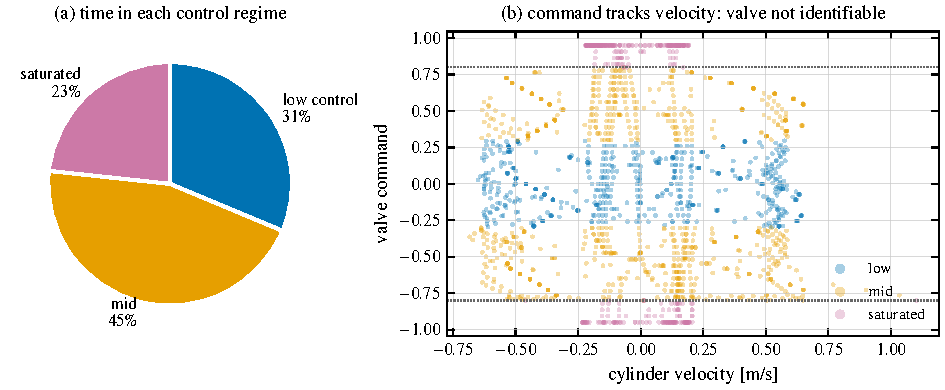
\includegraphics[width=\textwidth]{images/ch4_regimes}
  \caption{The closed-loop batch is diverse in control effort but
  not identifiable. (a)~Fraction of time the valve spends saturated, in the mid
  band and in low-command creep. (b)~The same run in the command--state plane,
  where the correlation that blocks identification is visible.}
  \label{fig:data:regimes}
\end{figure}

\subsection{Design of the Excitation Signal}

The excitation run lasts $\unit[64]{s}$ and follows the fixed schedule
in Figure~\ref{fig:data:design}(c). One second of startup is simulated
and then discarded, because the plant is settling from its initial
condition and those samples describe the initialisation rather than the
dynamics. Four sequential slots follow, each giving one cylinder ten
seconds of excitation followed by a half-second zero-command gap. The
gaps make the boundaries between single-axis segments unambiguous. A
twenty-second phase then drives all four channels at once, and a final
second of zero command closes the run. Commands are limited to
$\pm 0.90$ of full authority.

The most consequential design decision here is one that runs against the
textbook reflex. A persistently exciting input for a linear system is
usually a rapidly switching signal, and the first version of this
excitation was built that way. It was persistently exciting in the
formal sense and still produced poor data, because the cylinders
reversed before they had travelled anywhere: the commanded energy went
into repeatedly accelerating and decelerating the piston near one point
of the stroke instead of moving it through the workspace. The present
signal replaces fast switching with long full-authority plateaus during
the sequential phase and a slow, high-authority component during the
simultaneous phase, so that each cylinder traverses a
substantial part of its stroke while its valve is open. The simultaneous
phase additionally superimposes one slow near-square cycle across the
full twenty seconds with a distinct medium-frequency component on each
channel, and short raised-cosine ramps at entry and exit keep the
transitions differentiable.

The lesson generalises, and it is one this thesis would offer to anyone
identifying a hydraulic actuator: persistent excitation is a condition
on the input signal, but the quantity that decides whether a
\emph{cylinder} is identifiable is how much of the stroke the input covers. The two are not the same, and optimising the first
while ignoring the second produces data that passes the classical test
and still cannot support a model.

\subsection{Plant Draws and Acceptance}

The same excitation is applied to four plant draws taken from the same
parameter space as the closed-loop campaign: nominal, randomized
hydraulics, randomized mechanics, and fully randomized. Holding the
input fixed and varying only the plant is what makes the four runs
directly comparable, since any difference in the response is attributable
to the parameters.

Each run is checked for stroke coverage before it is accepted. The
collector requires at least $10\,\%$ of the available stroke on
cylinders 1--3 and $8\,\%$ on cylinder 4, warns below a target of
$30\,\%$, and records the achieved coverage per channel in the run
summary. The runs retained here cover between $12\,\%$ and $33\,\%$ of
the stroke depending on the cylinder, which is above the acceptance
floor but below the target. Cylinder 4 is the weakest, and improving its
coverage is the clearest available next step for this campaign.

One earlier excitation export was rejected outright rather than repaired.
Half of its runs turned out to contain duplicated state trajectories, so
the nominally distinct plant draws were not distinct in the data, and
the valve was again not causally identifiable. That export and its
reports are not part of the maintained workflow. It is mentioned here
because it is the reason the acceptance checks in
Section~\ref{sec:data:diagnostics} exist in their present form: they were
written to make that particular failure impossible to miss a second
time.

\section{Combining Closed-Loop and Open-Loop Datasets}
\label{sec:data:combining}

The two campaigns are complementary, and each learned model of
Chapter~\ref{chap:models} draws on them in a different proportion.

The inverse-dynamics model is trained entirely on closed-loop material,
because its target is the command a competent controller issued in a given
state. The forward-dynamics model begins there and is then retrained on the
strict open-loop export, with the closed-loop data retained as a replay term at
weight $0.25$. Ablation showed that dropping the replay term costs state
coverage and extension accuracy, because four excitation runs cannot span the
poses a thousand operating runs visit.

Figure~\ref{fig:data:coverage} shows why. The closed-loop distribution fills
the reachable range smoothly; the open-loop distribution concentrates into
narrow plateaus. The open-loop bands are where the valve is identifiable, the
closed-loop mass is where the model must be accurate at deployment, and neither
campaign covers both. The forward model is therefore trained on their union.

\begin{figure}[tb]
  \centering
  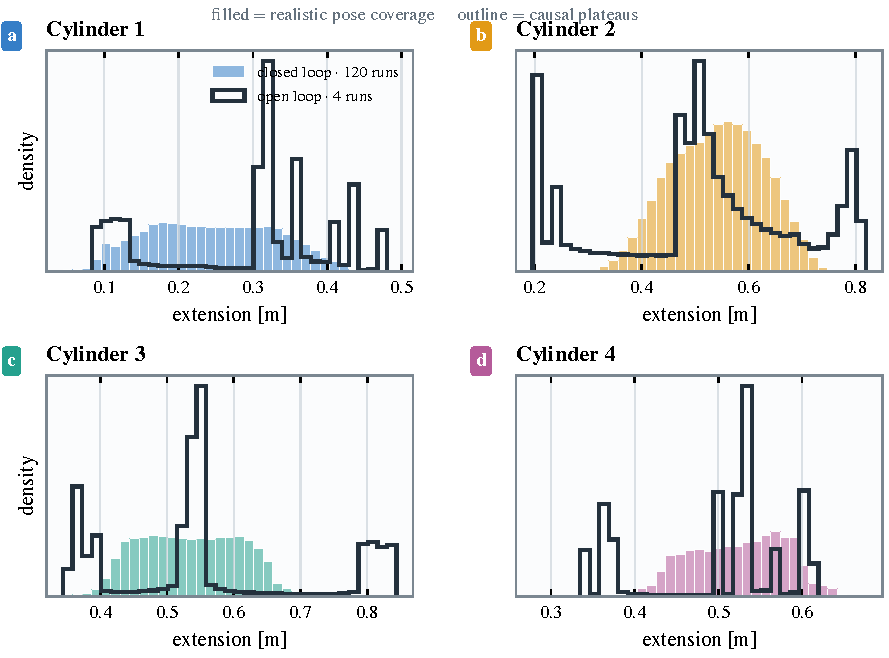
\includegraphics[width=\textwidth]{images/ch4_coverage}
  \caption{Extension coverage of the two campaigns, per cylinder
  and pooled over runs (closed-loop filled, open-loop outline). The closed-loop
  data fills the reachable range smoothly; the open-loop data concentrates into
  the plateaus where the valve is identifiable.}
  \label{fig:data:coverage}
\end{figure}

The reduced-order model consumes the closed-loop material in a joined
form. The inverse and forward exports are aligned on exact run
identifiers, time indices, and sample times, and the join is accepted
only when the sixteen-dimensional cylinder state agrees between them
sample for sample. The resulting command-conditioned dataset contains
$452\,400$ transitions at $\unit[0.05]{s}$ drawn from $1\,040$ aligned
runs. The logged valve command is carried through this join, but only as
a supervision target for the model's internal valve head. It is never a
runtime input, which is the property that lets the ROM be driven by
desired cylinder motion alone (Section~\ref{sec:models:rom}).

The thousand-run randomized curriculum described in
Section~\ref{sec:data:closed-loop} occupies a different position in the
argument, and I want to be exact about it because it is easy to
overstate. The inverse, forward, and reduced-order models reported in
Chapter~\ref{chap:models} were trained on the earlier aligned export,
which is a nominal-plant collection. The randomized curriculum was
collected under the earlier plan, in which randomized Simscape runs
would supply both the robust actuator variants and the privileged
factor vectors for latent adaptation. Neither role survives: the
adaptation evidence chain of this thesis is built entirely on the
IsaacLab collection of Section~\ref{sec:data:isaaclab}, for the reason
given there, and no result in this thesis is trained on or evaluated
against the randomized Simscape curriculum. It is reported as
provenance and as a negative methodological record, not as a substrate
whose consequences appear later.

\section{Closed-Loop Calibration Data for the Command ROM}
\label{sec:data:rom-calibration}

The reduced-order model is the one actuator model that does not stop at the
Simscape boundary. It is accurate about hydraulics, but the plant it drives at
runtime is a PhysX articulation with its own contact behaviour and compliance,
and the systematic offset between the extension the ROM commits to and the one
PhysX realizes is invisible to any amount of further Simscape training.

The calibration set is therefore collected from the deployment loop itself. A
previous ROM checkpoint is rolled out through the parked workflow of
Section~\ref{sec:sys:parked} on its five reference shapes, logged on the ROM's
own $\unit[0.05]{s}$ grid, giving $4\,084$ transitions. Each record stores the
six-step ROM history as the runtime assembles it, together with the measured
PhysX transition. The targets are what the plant did, not what Simscape said it
would do.

Two properties make the set safe to use. Only the bounded command-gated
correction head is trainable against it, with every other parameter frozen and
the correction capped at $\unit[3]{mm}$, so the identified physics is preserved
and only a deployment offset is added. And fine-tuning runs against a mixture,
replaying the original dataset at weight $0.25$, because five parked shapes
cannot span the poses a thousand Simscape runs visit. The correction is
command-gated and therefore exactly zero at zero command, so the stationary
hold contract survives unchanged.

One limitation is carried forward. The calibration data comes from the
\emph{parked} diagnostic workflow rather than the moving-verge task, so it
fits the actuator to PhysX under free-space tracking and not under
cutter--ground contact. The calibration is therefore weakest in the regime the
verge task spends most of its time in, and the bounded correction head keeps
that gap contained rather than closing it. This calibration is also what
qualifies the ROM as the deployment actuator, with the consequences for the
three-way comparison set out in Section~\ref{sec:sys:rom-is-plant}.

\section{The IsaacLab Adaptation Collection}
\label{sec:data:isaaclab}

\subsection{Provenance of the Adaptation Data}

The models that carry the adaptation argument
(the system-dynamics surrogate, the privileged factor encoder, and the
AAM) describe the plant that the adaptive controller is closed around. That
plant is not the Simscape model. It is the command ROM plus PhysX, the
same four-dimensional cylinder command port used at deployment. A
surrogate identified on Simscape data would be a model of a model, and
the latent it defines would describe variation the deployment plant does
not necessarily exhibit. The adaptation dataset is therefore collected
\emph{in} the deployment plant, and the frozen ROM, ID and FD
checkpoints enter this chain only as fixed components, never as things
to be retrained.

\subsection{The Physical Factor Vector}
\label{sec:data:factors}

The randomized quantity is a six-dimensional physical factor vector
%
\begin{equation}
  \label{eq:data:factorvec}
  \factorvec = \bigl[
    e_{\mathrm{flow}},\;
    e_{\mathrm{compliance}},\;
    e_{\mathrm{seal}},\;
    e_{\mathrm{pressure}},\;
    e_{\mathrm{mass}},\;
    e_{\mathrm{COM}_z}
  \bigr],
\end{equation}
%
with the ranges of Table~\ref{tab:data:factors}. Four coordinates are
hydraulic and two mechanical, which is what makes the hydraulic-only,
mechanical-only, and combined domains of
Section~\ref{sec:data:domains} separable. Each candidate was admitted
only after a one-factor sensitivity screen confirmed that moving it
alone produces a measurable change in cylinder extension, velocity,
pressure, or end-effector motion. Parameters whose effect could not be
measured, or which could not be varied safely, were rejected rather than
carried as decoration.



One omission is deliberate. Actuation delay is not a
randomized coordinate. Delay in this system is an \emph{emergent}
property of flow, compliance, and load rather than a free parameter, so
it is measured as a response property of each run
(Chapter~\ref{chap:evaluation}) instead of being supplied to any model
as a known factor. Handing an estimator a factor that the real machine
would never publish is the same mistake as handing it the true latent.

\subsection{Domains and Factor Design}
\label{sec:data:domains}

Runs are organized into five domains
(nominal, hydraulic-only, mechanical-only, combined-training, and an
\emph{unseen} combined-test domain), and one factor vector is fixed for a complete run, so that no
run mixes plants. Factor configurations are drawn with deterministic
scrambled Sobol sequences~\cite{sobol1967distribution} rather than
independent uniform sampling, with explicit boundary anchors so that the
corners of the space are represented and not merely approached, and with
fixed per-domain seeds so the design is reproducible independently of
the data it produced. Combined draws that compound into an excessive
response gain are rejected at draw time rather than being collected and
discarded later.

The resulting design is auditable: $98.3\,\%$ of the factor keys are
unique, the active-factor matrix is full rank, every factor quartile is
populated, and the factor keys of the training, validation, and test
splits are disjoint. That last property is the one that matters most for
the claims of Chapter~\ref{chap:evaluation}: a test run does not merely
come from a different episode, it comes from a plant the models have
never seen.

\subsection{Collection Procedure}

Every run is collected through the same interface the policy uses. The
DLS controller closes the loop on measured cylinder state and issues its
command through the four-dimensional action port into the command ROM
and PhysX. No joint-target bypass is used, and no PPO policy is used to
collect identification data, because a policy trained on the same plant
would reintroduce the closed-loop correlation that
Section~\ref{sec:data:open-loop} spent a campaign removing.

Independent excitation is supplied by dedicated four-channel PRBS
windows applied through that same action port, with a small amplitude
and a hold of ten control steps, so that the excitation is causally
independent of the state without ever leaving the safe envelope. Probe
actions are logged separately from controller output, so any analysis
can distinguish the two. Each run follows a fixed eleven-segment structure
(settle, three postures, three PRBS windows, DLS task motion,
reach-and-return, and stow), giving $11\,304$ control steps
and $\unit[188.4]{s}$ of simulated time per run. Three postures plus
line, coupled-sine, and reach-and-return motion were verified in a pilot
to give full rank over all four action channels under varied geometry
and load.

\subsection{The Frozen Dataset}

The final collection contains $118$ complete runs: $2$ nominal, $40$
hydraulic-only, $12$ mechanical-only, $48$ combined-training, and $16$
unseen combined-test. Collection ran in four vectorized IsaacLab
environments with per-environment factors and logging. Slots that
tripped a safety or validity check were discarded and retried
individually rather than being silently kept. All $118$ runs passed the
final collection gate, which checks finite physics, exact model-grid
alignment, command rank, factor-response authority, state coverage, and
saturation limits.

The dataset is then \emph{frozen}: the raw runs are checksummed and the
run-level split is fixed at $82$ training, $20$ validation, and $16$
reserved combined-test runs, with zero factor-key leakage between them.
The reserved sixteen are not touched again:
not for history-length selection, not for model selection, and not for
hyperparameter choices, so that the final adaptation claim is measured on material no decision
in this thesis was conditioned on.

\subsection{Learning Timebase and Hydraulic State}

The learning timebase is the actuator model grid, not the control clock.
Samples are exact $\unit[50]{ms}$ ROM transitions taken at control
indices $0, 3, 6, \dots$: state row $t$ and command row $t$ predict
state row $t+3$. Nothing is interpolated. This is the same alignment
rule as Section~\ref{sec:sys:timing}, and it is enforced rather than
assumed, because a model trained across a mismatched interval is wrong by a fixed factor in the quantity it exists to supply.

The hydraulic state used by the system-dynamics models is
%
\begin{equation}
  \label{eq:data:sdstate}
  \bm{s}_t = \bigl[\bm{x}_t^{1:4},\; \dot{\bm{x}}_t^{1:4},\;
  \Delta\bm{p}_t^{1:4}\bigr] \in \mathbb{R}^{12},
\end{equation}
%
with joint position and velocity carried as \emph{context} only, and the
prediction target the next $\unit[50]{ms}$ state delta. Differential
pressure occupies an awkward position in this design: it is
recorded, and it is a prediction target and a diagnostic, but it is
withheld from the final deployment-mirror input. A real machine does not
publish chamber pressure on this interface, so a model allowed to read
it would be validated under an assumption deployment cannot honour.
Withholding it is what makes a causal history \emph{belief} necessary
rather than optional, and that necessity is the whole reason the AAM has
work to do.

\section{Feature and Target Construction}
\label{sec:data:features}

\subsection{The Actuator Models}

The three learned actuator models take cylinder-space features, in the
ordering and notation fixed in Section~\ref{sec:models:overview}. Their
input contracts differ because their questions differ. The inverse model
receives the measured cylinder state, the logged rod forces, the desired
increments, and the previously applied command, twenty-eight numbers in
all. The forward model receives the applied valve command and the
measured state, twenty numbers. The reduced-order model receives a
six-sample history of state, previously predicted valve, and desired
command, twenty-four numbers per step.

Three conventions apply throughout, and they are the same ones the models
enforce at inference time.

\paragraph{Increment Targets}
Every dynamic target is a within-run one-step increment,
$\Delta \bm{x}_k = \bm{x}_{k+1} - \bm{x}_k$, never an absolute state.
This removes the large static component of the signals and, more
importantly, makes the trivial persistence solution an explicit baseline
that a model can be measured against rather than a hiding place it can
settle into.

\paragraph{Causal Alignment}
Features at step $k$ contain only quantities available at step $k$. The
extraction stage verifies this by recomputing every logged target from
the within-run difference of the states and requiring exact agreement,
a check reported in Section~\ref{sec:data:diagnostics}.

\paragraph{Time-Base Conversion}
The open-loop campaign is logged at $\unit[0.01]{s}$ but the models run
at $\unit[0.05]{s}$, so five consecutive raw samples are combined into a
single transition. The valve input attributed to that transition is the
command held at the start of the window, which is the causally correct
choice. The mean command over the window is also recorded, but only for
analysis. Cylinder extension velocity is not logged directly in the
closed-loop archive and is obtained by differentiating extension on the
output grid, which is consistent with the trapezoidal identity that the
strict data satisfies to $R^2 = 0.994$--$0.9997$
(Equation~\ref{eq:models:trapezoid}).

\subsection{Observable History of the Adaptation Models}
\label{sec:data:history-features}

The adaptation models draw their features from the frozen IsaacLab
collection, and here the interesting question is not what goes in but
what is kept out. A history window carries only quantities a deployed
machine could produce: the applied action, cylinder extension and
velocity, and joint position and velocity. Six classes of signal are
excluded by construction, and the exclusion is enforced by an explicit
input mask rather than by convention:

\begin{itemize}
  \item the physical factors $\factorvec$ and the true latent $\bm{z}$,
    because recovering them is the estimator's job;
  \item any future observation, because the estimator is causal;
  \item the hidden internal state of the command ROM, because the
    deployment interface does not expose it;
  \item the differential pressure $\Delta\bm{p}$, for the reason given
    in Section~\ref{sec:data:isaaclab};
  \item the desired task reference, so that the latent describes the
    plant rather than the trajectory being asked of it.
\end{itemize}

Windows are contained within a single run and never cross a run
boundary, and each window carries the stopped-gradient target
$\bm{z} = \mu(\factorvec)$ of its own run together with the run
identifier, domain, split, and valid history bounds. Applied to the
$118$ frozen runs this yields $444\,624$ causal history ticks. What is
built from them, how the history length is chosen, and how the result is
validated downstream belong to Chapter~\ref{chap:models}.

\section{Preprocessing and Data Splits}
\label{sec:data:preprocessing}

Splitting is done at the level of complete runs, never of individual
samples. A random sample-level split would place transitions from the
same trajectory on both sides of the boundary and report a validation
score that mostly measures interpolation within a run. For the
command-conditioned dataset the $1\,040$ runs are divided into $936$
training, $52$ validation, and $52$ test runs, giving $407\,160$,
$22\,620$, and $22\,620$ transitions respectively, with no run
identifier appearing in more than one split. The IsaacLab adaptation
collection is split by run \emph{and} by factor configuration
($82$/$20$/$16$, Section~\ref{sec:data:isaaclab}), which is the stronger
condition: separating runs alone would still let two runs of the same
plant fall on opposite sides of the boundary and turn a claim about
unseen plants into a claim about unseen episodes.

The strict open-loop export needs a different treatment because it
contains only four runs, and holding one out would remove an entire
plant draw from training. Instead each run is divided into twenty
temporal blocks, every fifth block is assigned to validation, and a
five-sample guard interval is discarded at each block boundary so that
no $\unit[0.05]{s}$ transition window spans the split. A simple
last-twenty-percent split was tried first and rejected: it changed the
spread of the targets between training and validation by a factor of
$1.3$ to $2.3$, because the final fifth of the run is the simultaneous
excitation phase and is dynamically unlike everything before it. That
split would have measured extrapolation to a different regime and called
it generalisation.

Normalization statistics are computed on the training split only and
stored inside each checkpoint, so that a model always normalizes with the
statistics it was fitted with. Mixing statistics between checkpoints
silently invalidates any comparison, and the loader enforces the stored
contract rather than recomputing it.

Finally, samples are carried with an explicit validity flag rather than
being silently dropped. In the strict export $93.7\,\%$ of samples are
marked valid. The remainder are the excluded startup and shutdown
seconds and the zero-command gaps. Keeping them in the archive with a
flag, instead of deleting them, means the time base stays contiguous and
the within-run difference checks remain meaningful.

\section{Dataset Diagnostics}
\label{sec:data:diagnostics}

No dataset in this thesis is used before it passes an explicit audit,
for the reason given at the end of
Section~\ref{sec:data:open-loop}. The audit of the strict open-loop
export is reproduced in Table~\ref{tab:data:audit}.



The two rank figures are the ones that speak directly to requirement R2.
The instantaneous command matrix has rank four, so no channel is a
linear combination of the others, and the lagged regressor matrix built
from the command history has rank eighty, so the excitation is
persistently exciting to the order the models need. The condition number
of that lagged matrix is about $4.6\times10^{3}$, which is finite and
workable rather than comfortable. It is a consequence of using long
plateaus, and it is the price paid for the stroke coverage those
plateaus buy.

The exactness of the three increment checks deserves a word, since a
maximum error of exactly zero invites suspicion. It is expected here:
the targets are computed from the logged states by the same within-run
difference that the check recomputes, so the check verifies that the
extraction stage did what it claims, not that the simulation is
accurate. It catches misalignment, off-by-one indexing, and rows that
have been reordered or concatenated across run boundaries, which are the failure modes that occur. Physical fidelity is a separate
question, addressed by the validation study in
Section~\ref{sec:sys:simscape-validation}.

Three limitations of the Simscape material are carried forward honestly.
Two limitations are carried forward. Stroke
coverage reaches only $12\,\%$ on the head-pivot cylinder, which is also the
cylinder the strict forward model predicts least well. The rod-force channel
fails a piston-area consistency check on this export, so it carries zero
supervised weight in the reduced-order model and no result rests on it.

The IsaacLab collection is audited against different failure modes. Design
adequacy is checked before use (unique factor keys, full active-factor rank,
disjoint keys across splits), physical validity per run (finite physics, exact
model-grid alignment, full command rank, bounded saturation), and leakage
structurally, with privileged channels removed by an explicit input mask rather
than by trusting the feature list. Its limitation is scale: $118$ runs over six
factors is a sparse design, which is why the adaptation claims of
Chapter~\ref{chap:evaluation} are reported with paired bootstrap intervals and
per-run detail rather than pooled point estimates.

With the data described and audited, the next chapter turns to what was
learned from it: the inverse and forward models that form the
\ppoIDFD{} actuator path, the command-conditioned reduced-order model
that replaces them in \ppoROM, and the system-dynamics, encoder, and
adaptation models built on the IsaacLab collection.

%%%%%%%%%%%%%%%%%%%%%%%%%%%%%%%%%%%%%%%%%%%%%%%%%%%%%%%%%%%%
%% Chapter 5 — Learned Models and Online Adaptation (14–22 pages)
%% Purpose: develop the learned actuator representations,
%% explain their training objectives, and establish the
%% distinction between robust modeling and explicit online
%% adaptation.
%%%%%%%%%%%%%%%%%%%%%%%%%%%%%%%%%%%%%%%%%%%%%%%%%%%%%%%%%%%%
\chapter{Learned Models and Online Adaptation}
\label{chap:models}

The previous chapter established how the Simscape datasets were generated and
why both closed-loop operation and open-loop valve excitation were required.
This chapter develops the learned actuator representations that consume those
datasets: the inverse-dynamics (ID) and forward-dynamics (FD) networks that
form the PPO1 actuator path, and the command-conditioned reduced-order model
(ROM) that replaces them in the PPO2 path. Each model is presented with its
exact input--output contract, architecture, training objective, and offline
validation evidence, because a recurring result of this work is that standard
supervised scores alone were not sufficient to accept any of these models: a
forward model can achieve near-perfect one-step $R^2$ while having learned
almost nothing about valve authority
(Section~\ref{sec:models:fd}). All models are trained on cylinder-space
signals only; the mapping between cylinder space and task space is handled by
the kinematic layers of Chapter~\ref{chap:system} and the control integration
is described in Chapter~\ref{chap:control}.

\section{Modeling Overview and Common Notation}
\label{sec:models:overview}

\subsection{Cylinder-space signals}

All learned models in this thesis operate on the four hydraulic cylinders of
the MULAG arm, indexed $i \in \{1,\dots,4\}$ in the fixed order slew cylinder
(\emph{Drehzapfen}), boom cylinder~I (\emph{Ausleger~I}), boom cylinder~II
(\emph{Ausleger~II}), and head pivot cylinder (\emph{Messerkopf-Schwenk}).
The passive fifth joint is not actuated and does not appear in any model
input. At the learned-model sample time $T = \unit[0.05]{s}$, the discrete
time index $k$ refers to the cylinder-space state
%
\begin{equation}
  \label{eq:models:state}
  \bm{x}_k \in \mathbb{R}^4, \qquad
  \dot{\bm{x}}_k \in \mathbb{R}^4, \qquad
  \Delta\bm{p}_k \in \mathbb{R}^4, \qquad
  \bm{F}_k \in \mathbb{R}^4,
\end{equation}
%
where $\bm{x}$ collects the cylinder extensions in meters, $\dot{\bm{x}}$ the
extension velocities, $\Delta\bm{p}$ the chamber pressure differences, and
$\bm{F}$ the logged rod forces. The valve command vector
$\bm{u}_k \in [-1,1]^4$ is the normalized spool command of the four
proportional valves. Desired quantities carry a star; the desired cylinder
command produced by the task controller is the pair
%
\begin{equation}
  \label{eq:models:command}
  \bm{c}_k = \bigl[\Delta\bm{x}^{*}_k,\; \Delta\dot{\bm{x}}^{*}_k\bigr]
  \in \mathbb{R}^{8},
\end{equation}
%
i.e.\ the extension increment and the extension-velocity increment that the
controller wants to realize over the next sample. Predictions of a model
carry a hat. Table~\ref{tab:models:notation} summarizes the notation used
throughout this chapter.

\begin{table}[tb]
  \centering
  \caption{Cylinder-space notation used by all learned models.}
  \label{tab:models:notation}
  \begin{tabular}{llp{7.6cm}}
    \toprule
    Symbol & Dimension & Meaning \\
    \midrule
    $T$ & -- & learned-model sample time, $\unit[0.05]{s}$ \\
    $\bm{x}_k$, $\dot{\bm{x}}_k$ & $\mathbb{R}^4$ & cylinder extension [m] and extension velocity [m/s] \\
    $\Delta\bm{p}_k$ & $\mathbb{R}^4$ & chamber pressure difference [Pa] \\
    $\bm{F}_k$ & $\mathbb{R}^4$ & logged rod force [N] \\
    $\bm{u}_k$ & $[-1,1]^4$ & normalized proportional-valve command \\
    $\bm{c}_k = [\Delta\bm{x}^*_k, \Delta\dot{\bm{x}}^*_k]$ & $\mathbb{R}^8$ & desired extension and velocity increments \\
    $\Delta(\cdot)_k = (\cdot)_{k+1} - (\cdot)_k$ & -- & within-run one-step increment \\
    $\hat{(\cdot)}$ & -- & model prediction \\
    $\bm{h}_k$ & $\mathbb{R}^{128}$ & recurrent latent state of the ROM encoder \\
    \bottomrule
  \end{tabular}
\end{table}

\subsection{Two actuator representations, one contract}

Figure~\ref{fig:models:overview} shows the two learned actuator paths side by
side. In the PPO1 path, actuation is represented by two separate networks:
the ID network maps the current hydraulic state and a desired increment to a
valve command, and the FD network maps a valve command and the current state
to the predicted state increment. Their composition
$f_{\mathrm{FD}} \circ f_{\mathrm{ID}}$ predicts what a commanded increment
will actually do to the cylinders. In the PPO2 path, one command-conditioned
ROM replaces this composition: it receives the same desired command
$\bm{c}_k$, predicts the valve internally, and propagates pressure, velocity,
and extension through an explicit, physically structured update
(Section~\ref{sec:models:rom}). Both paths terminate in the same bounded
PhysX cylinder position target inside the IsaacLab
environment~\cite{mittal2023orbit}, and both are driven by the same
damped-least-squares task controller and residual PPO
policy~\cite{schulman2017proximal,johannink2019residual} described in
Chapter~\ref{chap:control}. The experimental variable between PPO1 and PPO2
is therefore the actuator representation alone.

\begin{figure}[tb]
  \centering
  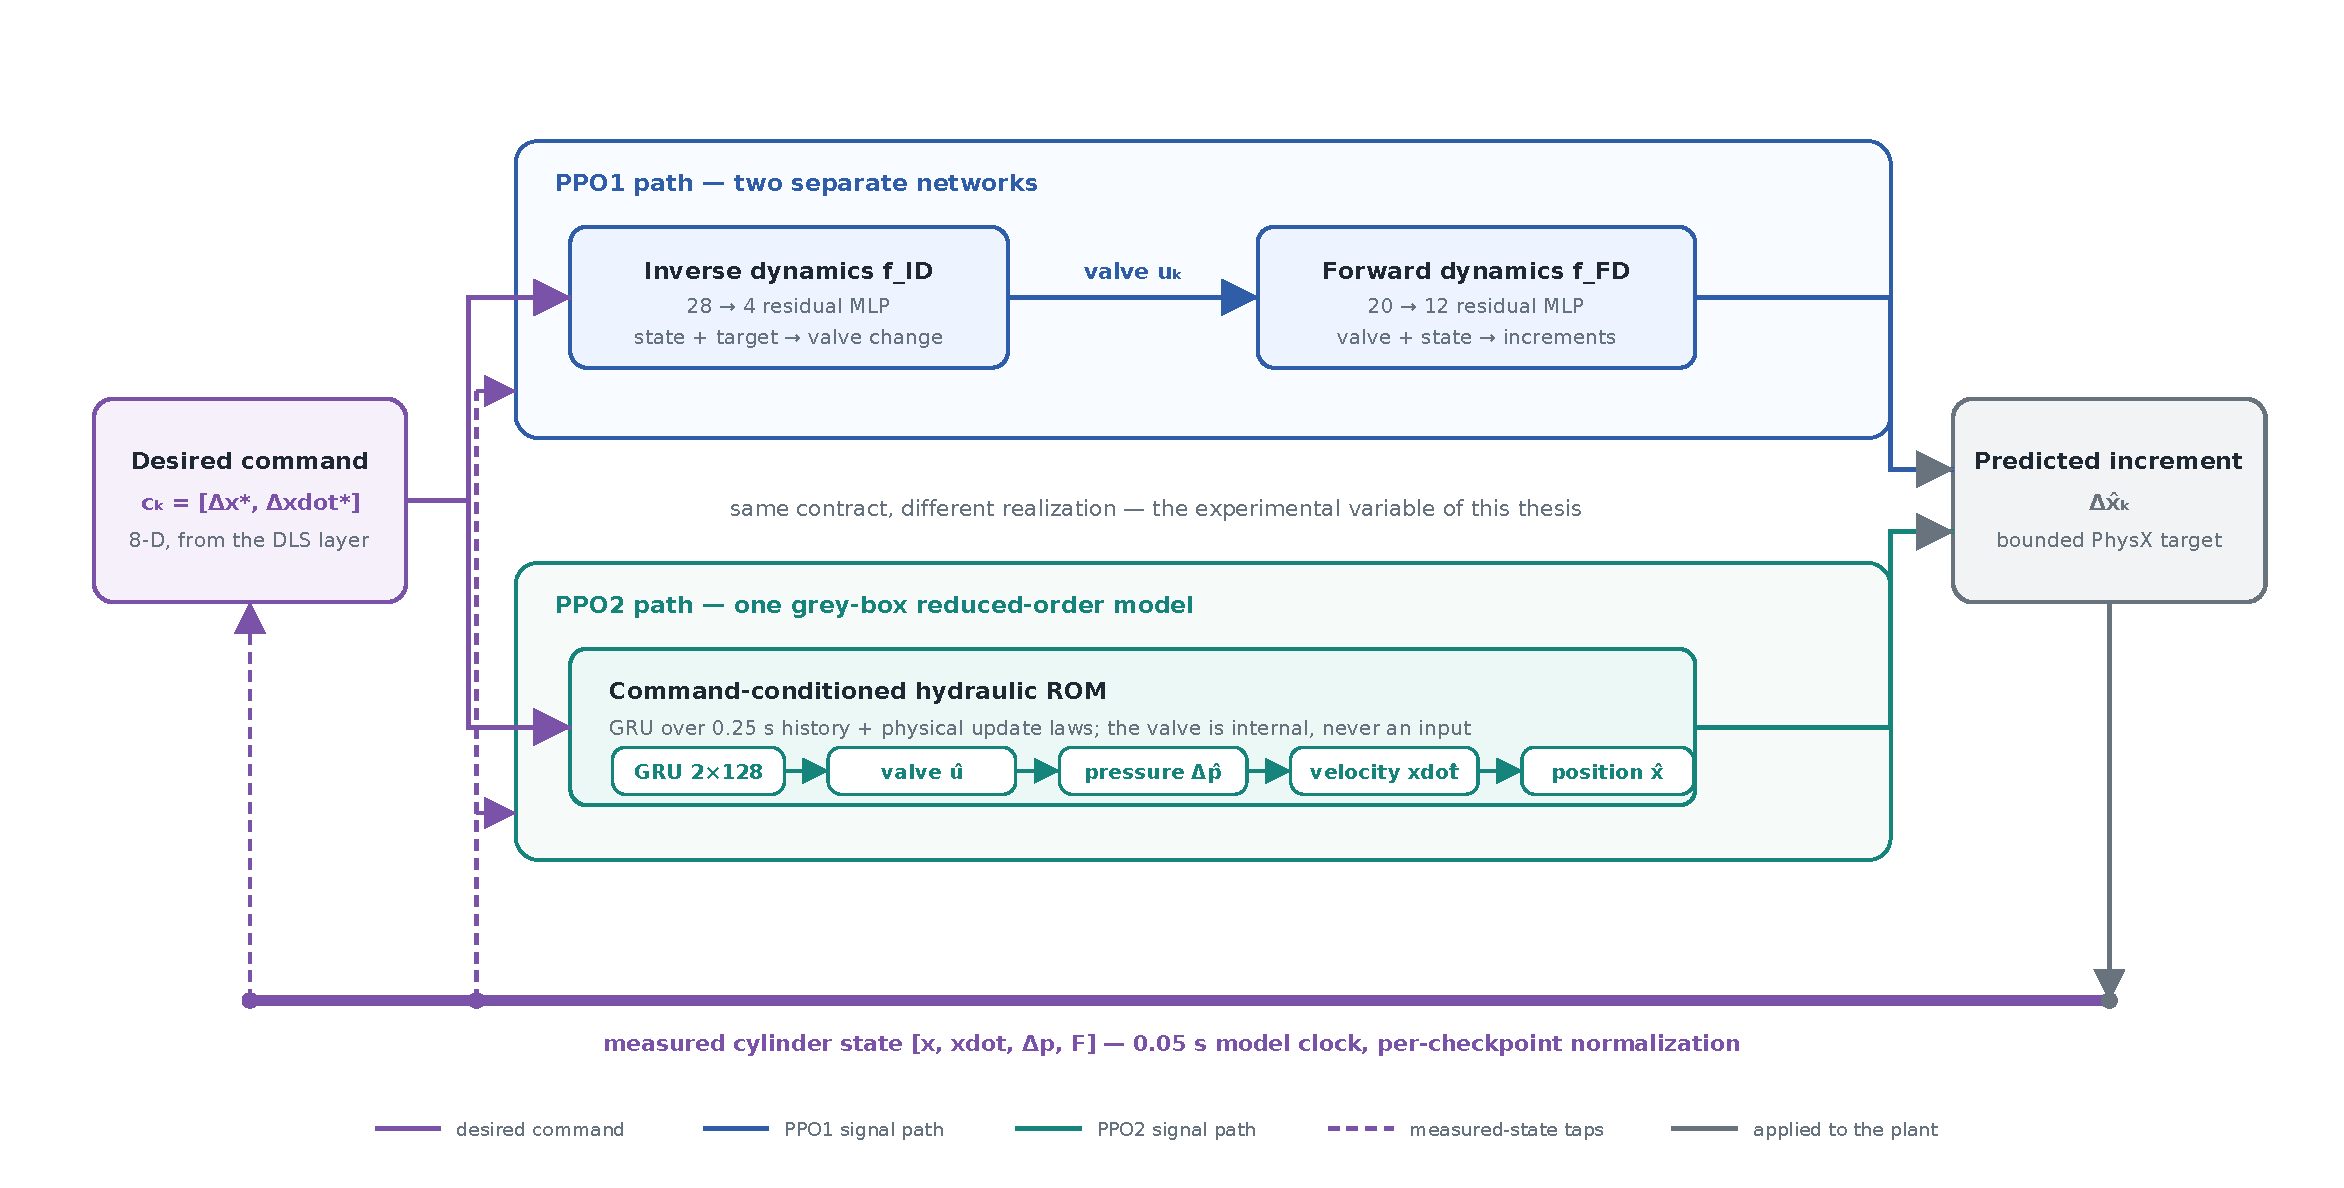
\includegraphics[width=\textwidth]{images/models_overview}
  \caption{The two learned actuator representations as parallel lanes
  around one shared contract. Both consume the same desired cylinder
  command and the same measured cylinder state from the feedback bus,
  and both produce the predicted increment that becomes the bounded
  PhysX target. The PPO1 lane composes two separately trained networks;
  the PPO2 lane realizes the command inside a single grey-box model
  whose valve signal is internal. Training-time data flow is described
  in Chapter~\ref{chap:data}.}
  \label{fig:models:overview}
\end{figure}

\subsection{Common conventions}

Three conventions apply to every model in this chapter.

\paragraph{Increment targets.}
All dynamic targets are within-run one-step increments,
$\Delta \bm{x}_k = \bm{x}_{k+1} - \bm{x}_k$, never absolute states. This
removes the dominant static component of the signals and makes the
persistence solution ($\Delta\hat{\bm{x}} = \bm{0}$) an explicit, testable
baseline rather than a hidden local minimum.

\paragraph{Per-checkpoint normalization.}
Every checkpoint stores the mean $\bm{\mu}$ and standard deviation
$\bm{\sigma}$ of its own training inputs and targets, and inference
normalizes each feature as
%
\begin{equation}
  \label{eq:models:norm}
  \tilde{\xi} = \frac{\xi - \mu_\xi}{\sigma_\xi}.
\end{equation}
%
Statistics are never shared between checkpoints; mixing the statistics of two
checkpoints silently invalidates any comparison between them, so the loader
enforces the stored contract.

\paragraph{Causal timing.}
Model inputs at step $k$ contain only quantities available at step $k$
(including the previously applied command), and targets are the measured
transition to step $k+1$. During dataset construction this alignment is
checked explicitly against the within-run differences of the logged states
(Chapter~\ref{chap:data}).

\paragraph{Gate-based acceptance.}
Finally, no model in this thesis is promoted on a supervised score.
Every candidate passes the fixed gate sequence of
Figure~\ref{fig:models:acceptance}: offline accuracy, input-ablation
authority, in-simulator cylinder gates, and the task-space tracking
gate, in that order. Each ``no'' exit names the repair that experience
showed to be the right one, and the promoted checkpoints are recorded
with their hashes for provenance. The sections that follow report, for
each model, exactly where in this ladder it initially failed and what
fixed it.

\begin{figure}[tb]
  \centering
  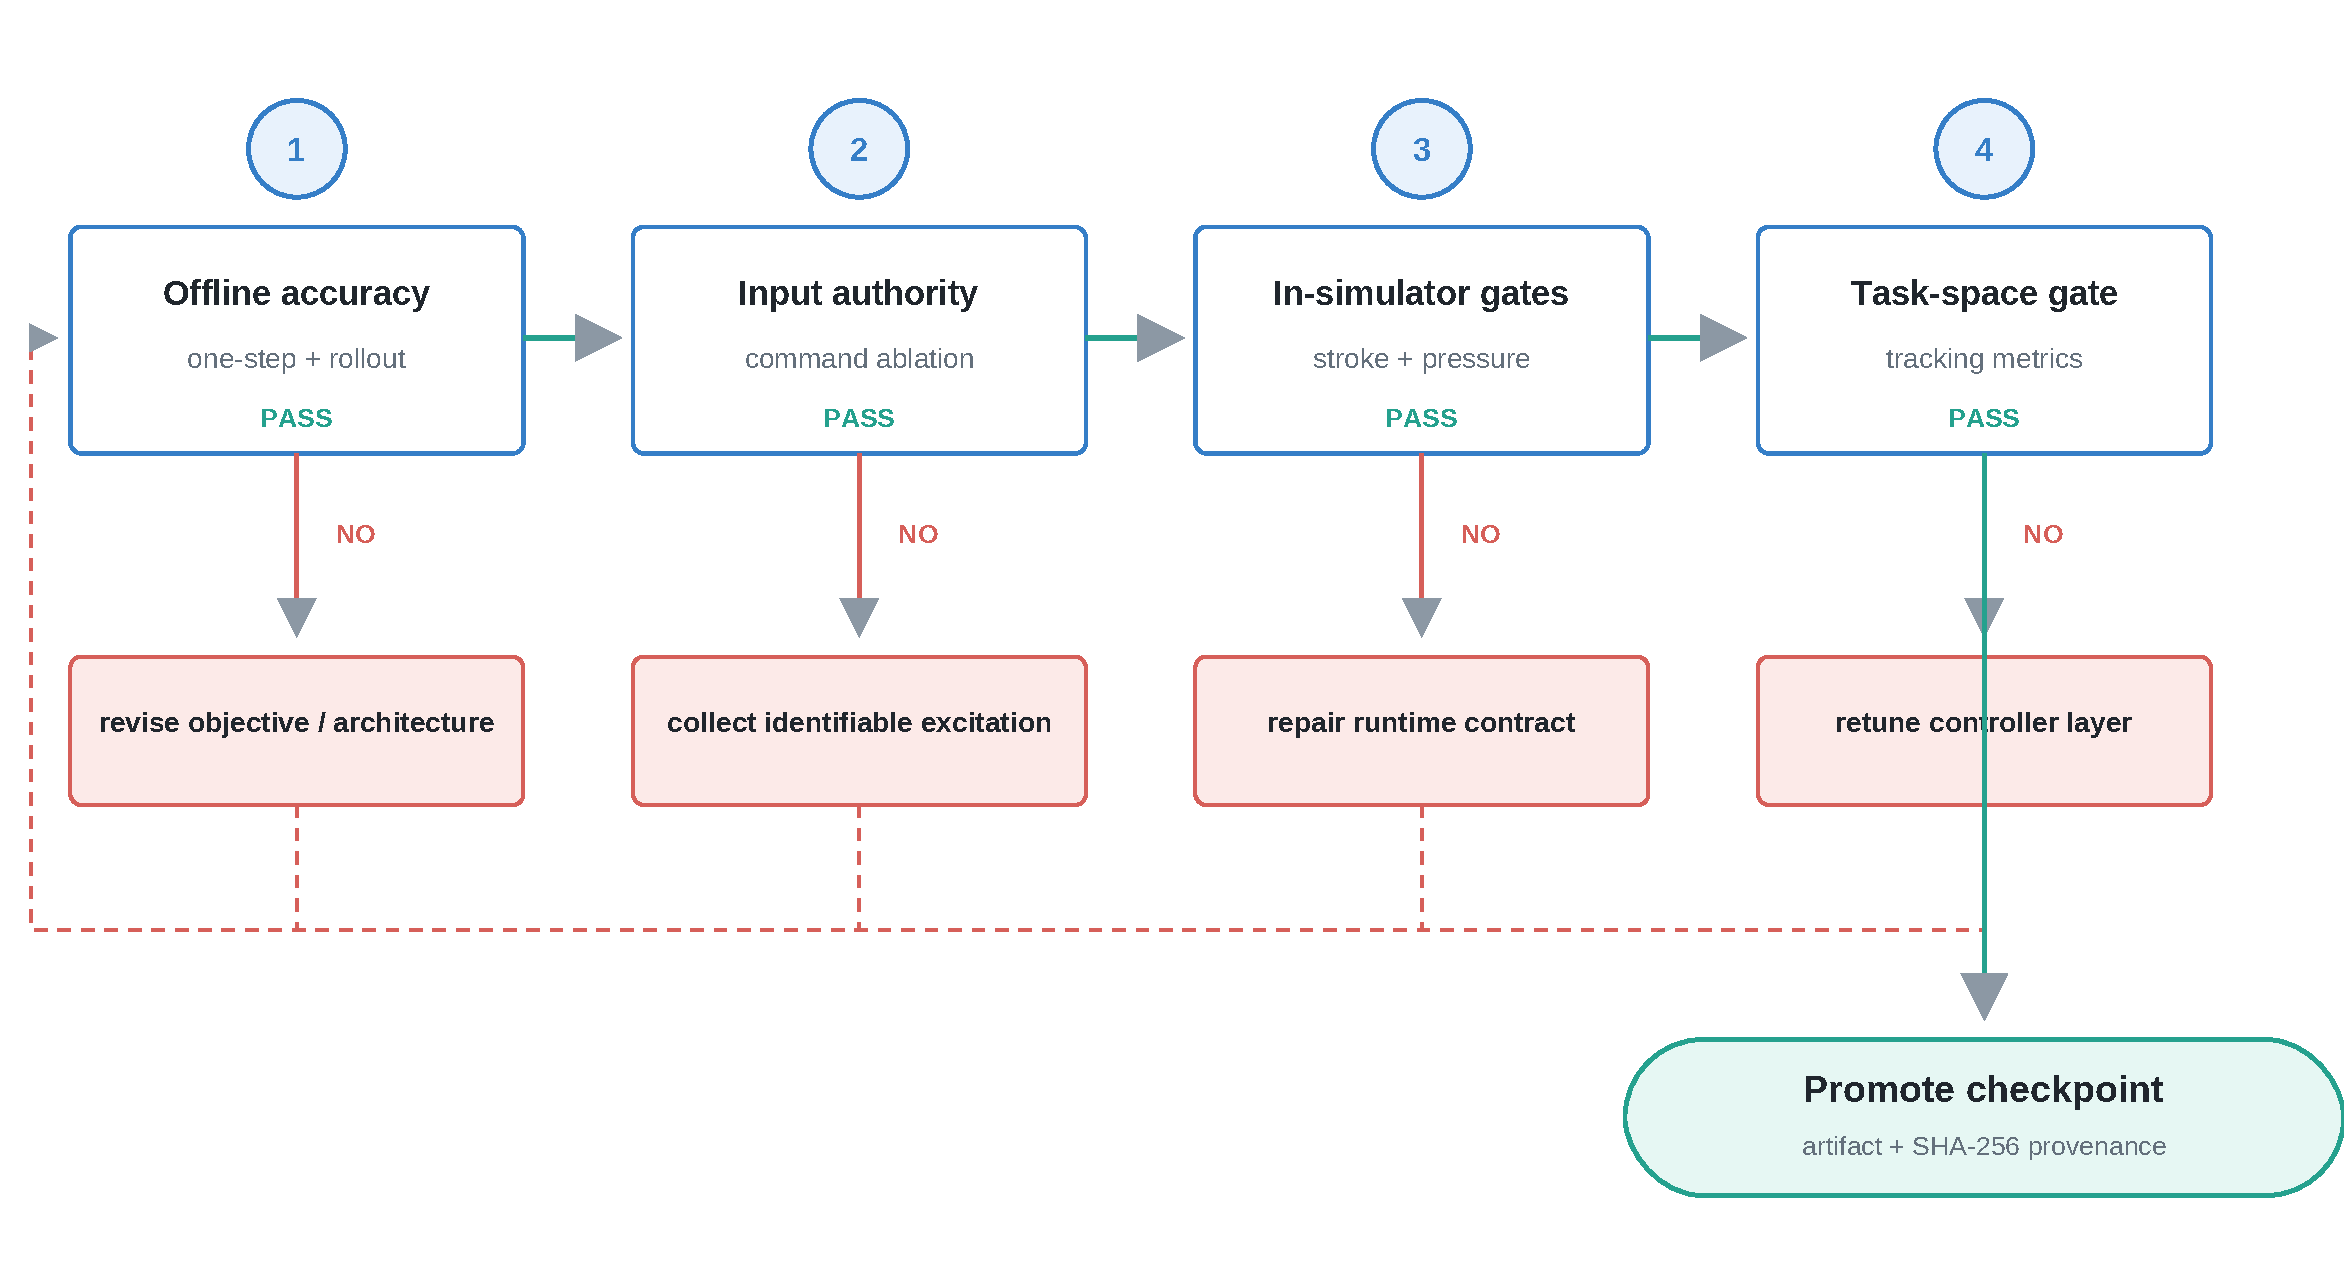
\includegraphics[width=.8\textwidth]{images/models_acceptance_flow}
  \caption{The acceptance ladder that every learned model in this
  thesis must climb before deployment. A candidate that fails a gate
  exits right into the corresponding repair loop and re-enters from the
  top; only a candidate that passes all four gates is promoted, and the
  promoted artifact is recorded together with its SHA-256 hash.}
  \label{fig:models:acceptance}
\end{figure}

\subsection{Data provenance in brief}

Two dataset families from Chapter~\ref{chap:data} are consumed here. The
\emph{closed-loop} family consists of the aligned Simscape
exports~\cite{mathworks2024simscape} used for supervised ID and FD training
and, after exact run-and-timestamp alignment, for the command-ROM dataset:
$452\,400$ transitions at $T=\unit[0.05]{s}$ from $1\,040$ runs, split by
complete runs into $936$ training, $52$ validation, and $52$ test runs
($407\,160$ / $22\,620$ / $22\,620$ samples). The \emph{open-loop} family is
the strict valve-excitation export used to repair the FD model: four $64$-s
runs sampled at $\unit[0.01]{s}$, in which the same rank-4 multi-input
open-loop excitation is applied to four distinct plant draws
(nominal, randomized hydraulics, randomized mechanics, both). Its properties
and the reasons it was necessary are analyzed in
Section~\ref{sec:models:fd}.

\section{Inverse Dynamics Model}
\label{sec:models:id}

\subsection{Input--output contract}

The ID network answers the question the low-level controller actually asks:
\emph{given the current hydraulic state, which valve command realizes a
desired cylinder increment?} Its contract is
%
\begin{equation}
  \label{eq:models:id-contract}
  \Delta\bm{u}_k = f_{\mathrm{ID}}
  \bigl(\bm{x}_k,\, \dot{\bm{x}}_k,\, \Delta\bm{p}_k,\, \bm{F}_k,\,
        \Delta\bm{x}^{*}_k,\, \Delta\dot{\bm{x}}^{*}_k,\, \bm{u}_{k-1}\bigr)
  \in \mathbb{R}^4 ,
\end{equation}
%
a 28-dimensional input mapped to a valve-command \emph{change}. The deployed
command is the accumulated
%
\begin{equation}
  \label{eq:models:id-apply}
  \bm{u}_k = \operatorname{clip}\bigl(\bm{u}_{k-1} + \Delta\bm{u}_k,\;
  -\bm{u}_{\max},\, \bm{u}_{\max}\bigr),
  \qquad \bm{u}_{\max} = [0.95,\, 0.95,\, 0.8,\, 0.8],
\end{equation}
%
where the per-axis limits are stored in the checkpoint. Predicting the
command change rather than the absolute command conditions the problem on the
previous operating point of the valve, which matters because proportional
valves are direction- and history-dependent around their dead zone
(Section~\ref{sec:fund:actuation-chain}). The desired increments
$\Delta\bm{x}^{*}, \Delta\dot{\bm{x}}^{*}$ in the training data are the
\emph{achieved} transitions of the logged Simscape runs, used as a proxy for
desired motion because no independent cylinder-space reference was logged;
the consequences of this proxy are examined below.

\subsection{Architecture and supervised training}

$f_{\mathrm{ID}}$ is a multilayer perceptron with an input projection to
width 512 followed by four residual blocks~\cite{he2016deep} with SiLU
activations~\cite{elfwing2018sigmoid}, layer
normalization~\cite{ba2016layer}, and dropout of
$0.02$~\cite{srivastava2014dropout}, implemented in
PyTorch~\cite{paszke2019pytorch};
Figure~\ref{fig:models:nn-architectures}(a) shows the trunk, which the
FD network shares, and Figure~\ref{fig:models:nn-architectures}(b) the
recurrent encoder that the ROM uses instead
(Section~\ref{sec:models:rom}).

\begin{figure}[tb]
  \centering
  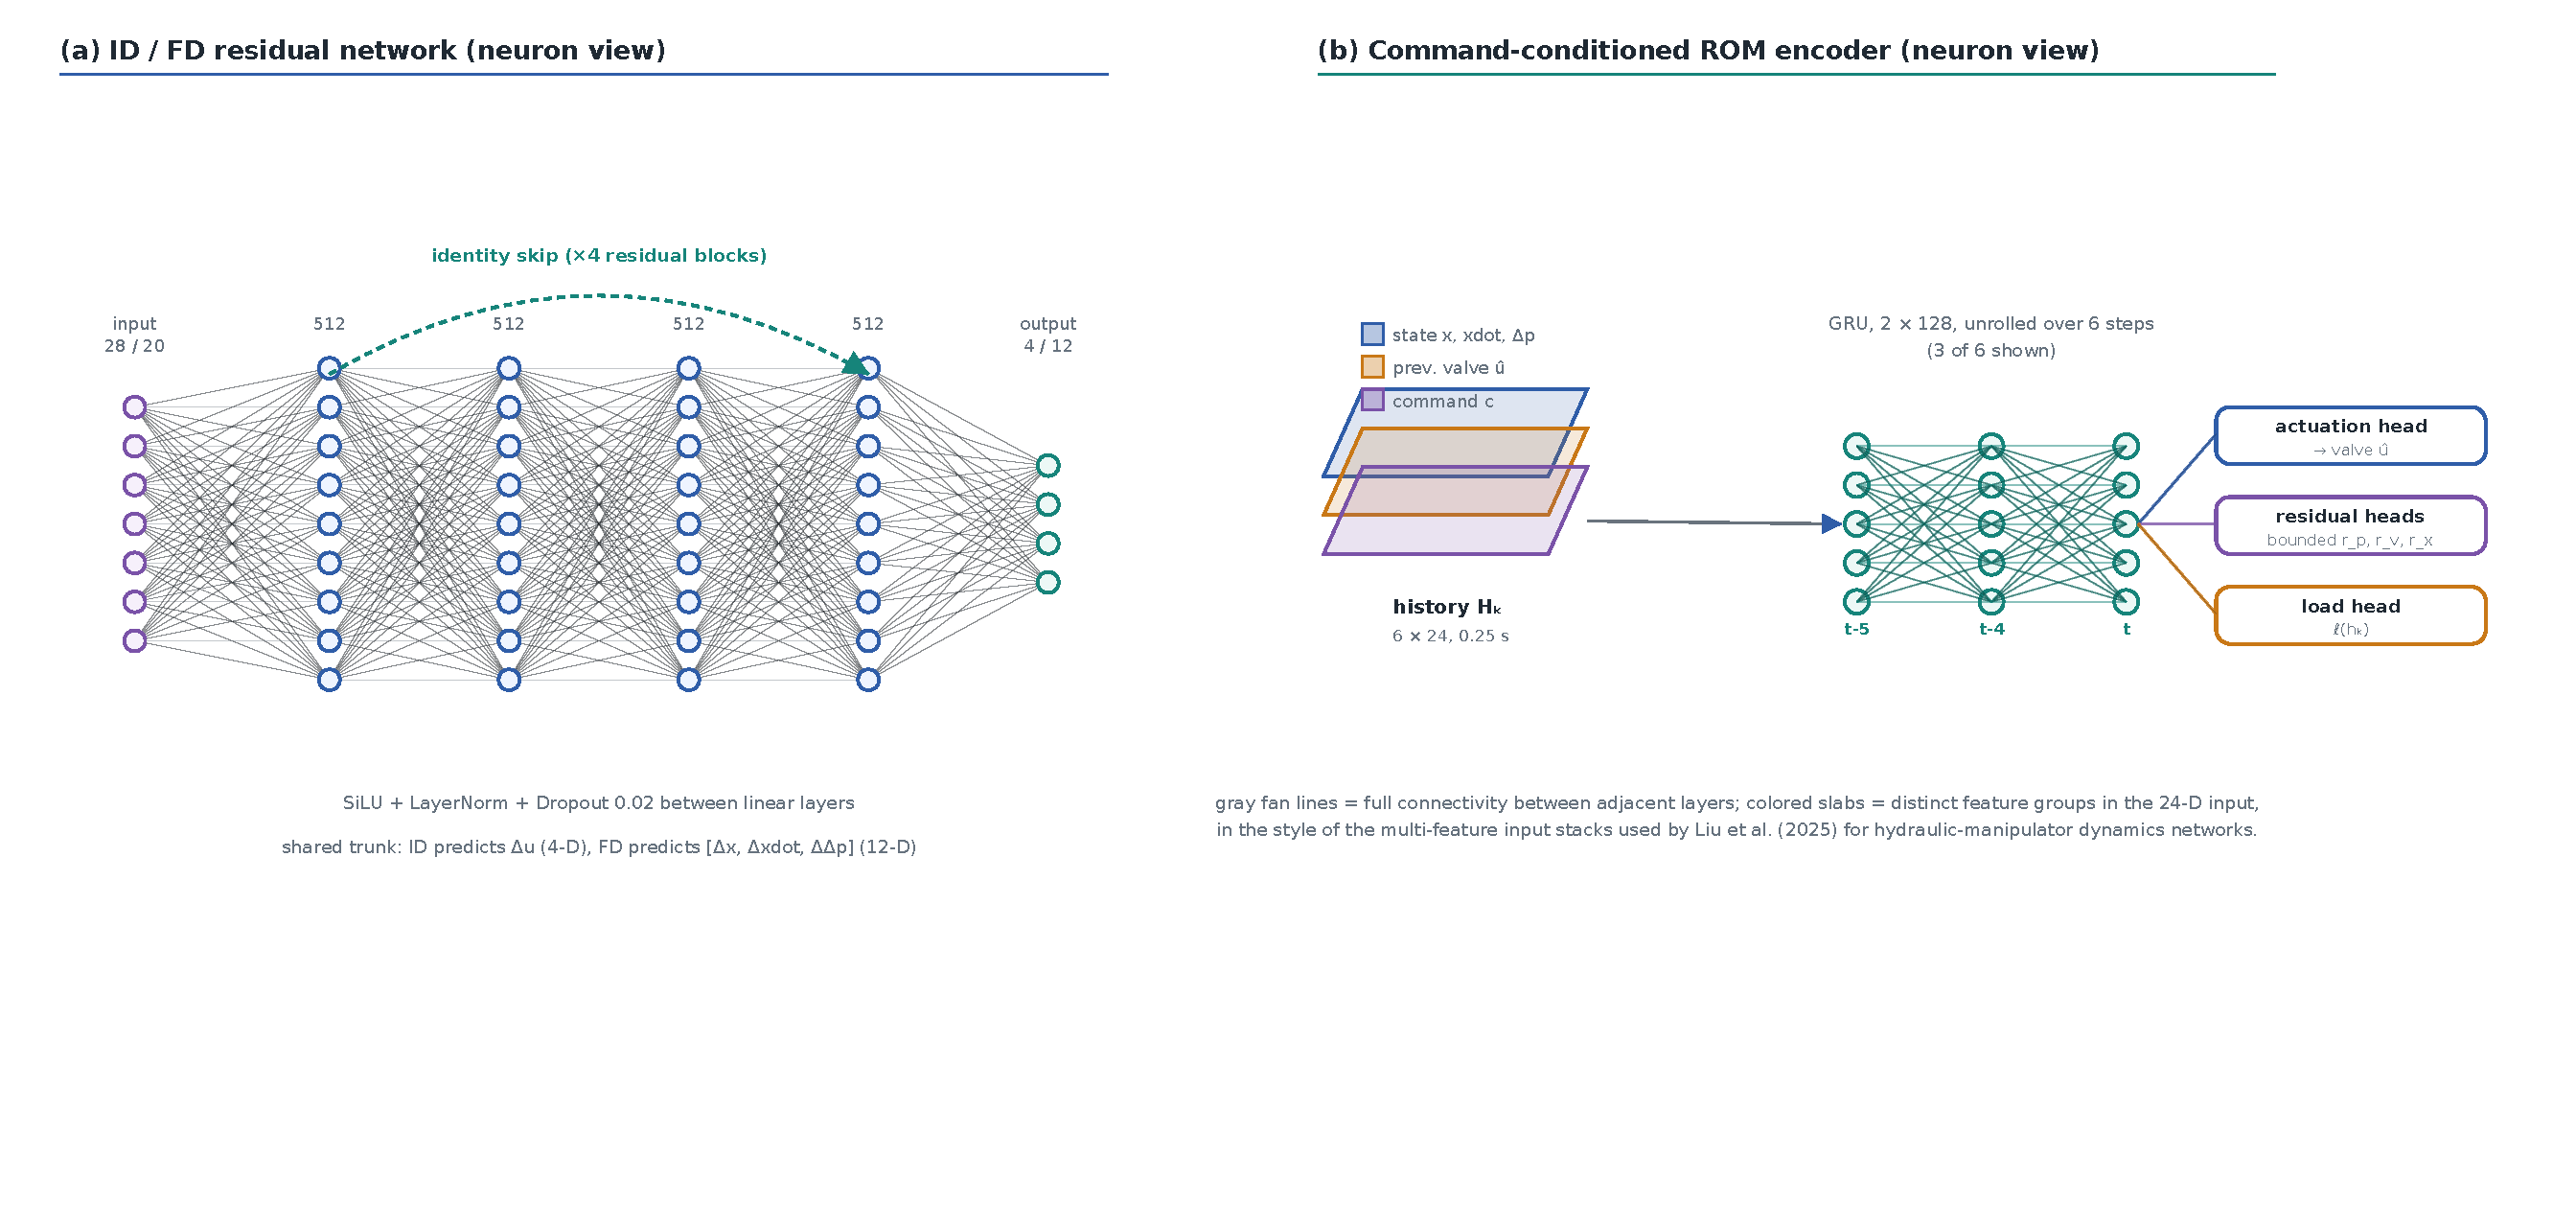
\includegraphics[width=\textwidth]{images/models_nn_architectures}
  \caption{The two network families used by the learned actuator
  models. (a)~The residual MLP trunk shared by the ID and FD networks:
  an input projection to width 512, four pre-activation residual blocks
  (Linear--LayerNorm--SiLU--Dropout--Linear with an identity skip), and
  a linear output head; only the input and output widths differ between
  ID and FD. (b)~The ROM's recurrent encoder, unrolled over its six
  history steps: each step consumes the 24-D feature vector, the hidden
  state carries pressure and command transients across time, and the
  final latent $\bm{h}_k$ feeds the actuation, residual, and load
  heads.}
  \label{fig:models:nn-architectures}
\end{figure} Training minimized the smooth-$L_1$ (Huber)
loss~\cite{huber1964robust} with transition point $\beta=0.5$ on normalized
targets using Adam~\cite{kingma2015adam} with learning rate $10^{-3}$, weight
decay $10^{-4}$, batch size $8\,192$, gradient-norm clipping at $10$, and
early stopping with patience $45$; samples in valve saturation were
up-weighted by a factor $1.25$ so that the rare saturated regime is not
ignored. The promoted checkpoint (seed 42) was selected at epoch 120 of at
most 300 with a validation loss of $0.0336$.

The supervised result was, on its face, excellent: per-valve validation
$R^2$ of $0.9996$, $0.9973$, $0.9981$, and $0.9974$. It must be stated
clearly what this number does and does not mean. It means the network
reproduces the logged valve commands from the logged states and achieved
transitions. It does not mean the composite map
$f_{\mathrm{FD}} \circ f_{\mathrm{ID}}$ has authority over the plant: since
the achieved transitions in closed-loop data are themselves produced by the
logged commands, a model can score highly by exploiting this correlation
without ever being asked to \emph{cause} a transition that was not already in
the data (Section~\ref{sec:fund:identifiability}).

\subsection{Paired control fine-tuning}
\label{sec:models:id-paired}

This deficiency became measurable when the ID and FD networks were composed.
For control, the relevant object is the \emph{paired differential response}:
the difference between what the FD predicts under the ID's command for the
actual target and under the ID's command for a zero target,
%
\begin{align}
  \bm{u}^{\mathrm{tgt}}_k &= f_{\mathrm{ID}}(\cdot,\, \bm{c}_k,\, \bm{u}_{k-1}),
  \qquad
  \bm{u}^{0}_k = f_{\mathrm{ID}}(\cdot,\, \bm{0},\, \bm{u}_{k-1}), \notag \\
  \Delta\hat{\bm{x}}^{\mathrm{pair}}_k &=
    f_{\mathrm{FD}}\bigl(\bm{u}^{\mathrm{tgt}}_k, \cdot\bigr)
  - f_{\mathrm{FD}}\bigl(\bm{u}^{0}_k, \cdot\bigr).
  \label{eq:models:paired}
\end{align}
%
If the pipeline is to be useful, $\Delta\hat{\bm{x}}^{\mathrm{pair}}_k$ must
track the requested $\Delta\bm{x}^{*}_k$. Before fine-tuning it did not: the
normalized control error of the composite was $1.00$ --- exactly the score of
predicting nothing --- with per-axis regression slopes of at most $0.004$
(Table~\ref{tab:models:paired}). Both networks were therefore fine-tuned
jointly on the control objective
%
\begin{equation}
  \label{eq:models:paired-loss}
  \mathcal{L}_{\mathrm{ctl}} =
  \bigl\| \Delta\hat{\bm{x}}^{\mathrm{pair}}
        - \Delta\bm{x}^{*} \bigr\|^2_{\mathrm{norm}}
  \;+\; \lambda_{\mathrm{ID}}\,\mathcal{L}_{\mathrm{ID}}
  \;+\; \lambda_{\mathrm{FD}}\,\mathcal{L}_{\mathrm{FD}},
\end{equation}
%
where the supervised losses $\mathcal{L}_{\mathrm{ID}}$ and
$\mathcal{L}_{\mathrm{FD}}$ are retained to limit regression from the
original data contracts. Crucially, the target blocks
$(\Delta\bm{x}^{*}, \Delta\dot{\bm{x}}^{*})$ were shuffled across valid
states during this stage, so the networks could no longer succeed by
reconstructing the logged trajectory; they had to respond to targets that the
logged controller never issued in that state.

\begin{table}[tb]
  \centering
  \caption{Effect of paired control fine-tuning on the composite
  $f_{\mathrm{FD}} \circ f_{\mathrm{ID}}$ differential response
  \eqref{eq:models:paired}, evaluated per cylinder axis on validation data.
  Before fine-tuning, the composite had essentially no control authority
  despite near-perfect supervised scores of both networks; the composite
  normalized control MSE fell from $1.0011$ to $0.1086$.}
  \label{tab:models:paired}
  \begin{tabular}{lcccc}
    \toprule
    & \multicolumn{2}{c}{Regression slope}
    & \multicolumn{2}{c}{Correlation} \\
    \cmidrule(lr){2-3} \cmidrule(lr){4-5}
    Cylinder axis & before & after & before & after \\
    \midrule
    1 (slew)      & $0.003$ & $0.818$ & $0.135$ & $0.920$ \\
    2 (boom I)    & $0.002$ & $0.928$ & $0.090$ & $0.967$ \\
    3 (boom II)   & $0.001$ & $0.849$ & $0.037$ & $0.933$ \\
    4 (head pivot)& $0.004$ & $0.912$ & $0.249$ & $0.958$ \\
    \bottomrule
  \end{tabular}
\end{table}

After 30 epochs of paired tuning the composite control MSE dropped to
$0.109$ and all four axes reached slopes above $0.8$ and correlations above
$0.92$. The resulting ID checkpoint
(\texttt{best\_id\_cylinder\_control.pt}) is the ID model deployed in all
PPO1 experiments. The fine-tuned FD from this stage, in contrast, was
accepted only as an intermediate: its remaining weakness under genuinely
independent valve excitation is the subject of the next section.

\section{Forward Dynamics Model}
\label{sec:models:fd}

\subsection{Input--output contract and supervised baseline}

The FD network predicts the one-step cylinder response to a valve command,
%
\begin{equation}
  \label{eq:models:fd-contract}
  \bigl[\Delta\hat{\bm{x}}_k,\; \Delta\hat{\dot{\bm{x}}}_k,\;
        \Delta\widehat{\Delta\bm{p}}_k\bigr]
  = f_{\mathrm{FD}}\bigl(\bm{u}_k,\, \bm{x}_k,\, \dot{\bm{x}}_k,\,
    \Delta\bm{p}_k,\, \bm{F}_k\bigr) \in \mathbb{R}^{12},
\end{equation}
%
a 20-dimensional input mapped to the three groups of state increments over
$T=\unit[0.05]{s}$. The architecture is the same residual MLP trunk as the ID
network (width 512, four residual blocks, SiLU, layer normalization, dropout
$0.02$). Supervised pretraining on the closed-loop Simscape export used
normalized MSE on all three output groups, Adam with learning rate
$10^{-4}$, weight decay $10^{-4}$, batch size $8\,192$, and an auxiliary
recursive rollout loss (weight $0.25$, horizons of 2, 5, 10, and 20 steps),
with the checkpoint selected by validation rollout
loss~\cite{nagabandi2018neural}. The selected model (epoch 291) reached
grouped one-step $R^2$ near $0.999$ for the extension increments.

\subsection{Why the supervised score was not believed}
\label{sec:models:fd-identifiability}

A model intended to give a policy gradient information about actuation must
respond to the \emph{valve}, not merely to the state history. This property
was tested directly with an input ablation: zeroing the valve input of the
pretrained FD barely changed its long-horizon rollout error
(valve-zero error ratio $\approx 0.94$ at a $\unit[0.5]{s}$ horizon;
Figure~\ref{fig:models:fd-authority}, dashed orange versus solid orange).
The model had learned to extrapolate the smooth kinematics of closed-loop
operation --- effectively a sophisticated persistence model --- because in
feedback data the controller makes valve command and state history nearly
redundant, the identifiability trap of
Section~\ref{sec:fund:identifiability}. Ablation
studies on the source MAT exports (Chapter~\ref{chap:data}) confirmed that
the valve signal was not causally identifiable from the closed-loop
distribution at all. No amount of retraining on the same distribution could
fix this; the data had to change.

\subsection{Strict open-loop excitation dataset}
\label{sec:models:fd-strict}

The repair dataset is the strict open-loop excitation export shown in
Figure~\ref{fig:models:excitation}. All four valves receive a rank-4
multi-input open-loop sequence built from long, full-authority command
plateaus: the first four segments excite one cylinder at a time, and the
final segment drives all four channels simultaneously
(Section~\ref{sec:data:open-loop}). The same excitation is applied to
four distinct plant draws --- nominal, randomized hydraulics, randomized
mechanics, and both randomized --- giving four $64$-s runs at
$\unit[0.01]{s}$ ($6\,400$ samples each, 49 logged columns). Dataset
validation established the properties that the closed-loop export lacked:
all four state trajectories are distinct; every logged target increment
agrees with the within-run difference $\bm{x}_{k+1}-\bm{x}_k$; valve history
alone predicts the pressure response with $R^2 \approx 0.80$--$0.85$; the
valve regressors have variance-inflation factors of only 7--10; and
pressure-relief saturation occupies 9--22\,\% of the samples, so the
saturated regime is represented but not dominant. An earlier excitation
export was rejected outright because half of its runs duplicated state
trajectories and the valve was again not causally identifiable --- a reminder
that excitation data must itself be audited, not assumed
informative~\cite{isermann2011identification}.

\begin{figure}[tb]
  \centering
  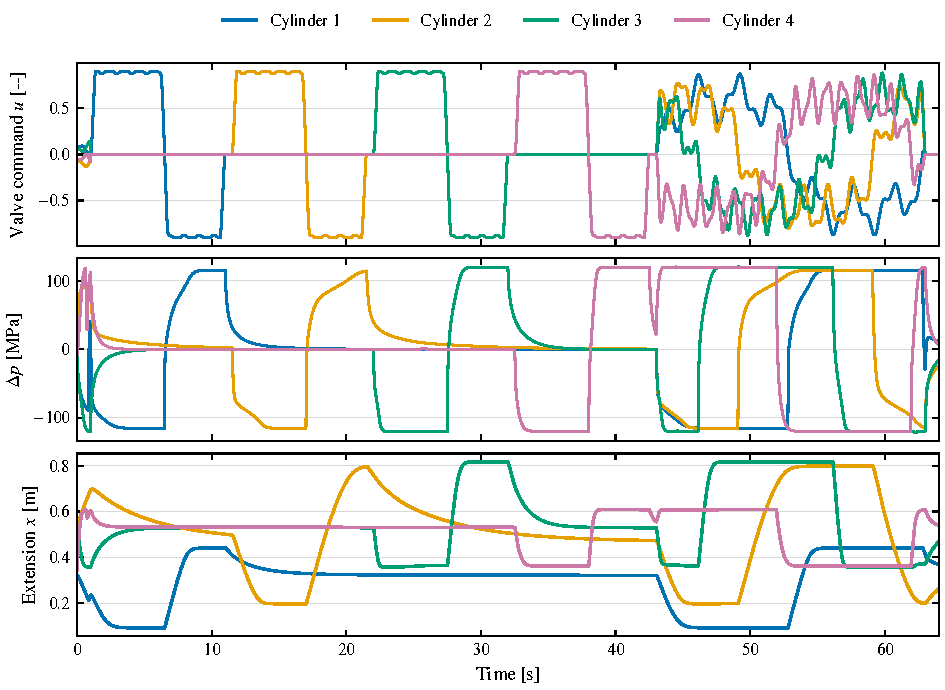
\includegraphics[width=\textwidth]{images/ch5_excitation_dataset}
  \caption{One run of the strict open-loop excitation dataset (nominal plant
  draw, $\unit[0.01]{s}$ sampling). Top: the rank-4 open-loop valve
  commands; the channels are excited individually in the first four segments
  and simultaneously in the final segment. Middle: resulting chamber
  pressure differences, including relief-limit episodes. Bottom: cylinder
  extension responses. The same excitation is repeated on three further
  randomized plant draws.}
  \label{fig:models:excitation}
\end{figure}

For FD training, five consecutive $\unit[0.01]{s}$ samples are combined into
one $\unit[0.05]{s}$ transition, with the valve input taken as the command
held at the beginning of the window. Each run is divided into 20 temporal
blocks with every fifth block assigned to validation and five-sample guard
intervals removed at each boundary, so no transition window crosses a split
boundary while train and validation samples still cover comparable pose and
energy regimes. A plain last-20\,\% split was tried and rejected because it
changed the target spread between train and validation by a factor of
1.3--2.3 and would therefore have tested extrapolation to a different
operating regime rather than generalization within one.

\subsection{Strict retraining objective}

Starting from the paired-control FD checkpoint, the promoted retraining run
(150 epochs, Adam, learning rate $3\times10^{-4}$) minimized
%
\begin{equation}
  \label{eq:models:fd-strict-loss}
  \mathcal{L}_{\mathrm{FD}} =
    \mathcal{L}_{\mathrm{Huber}}^{\mathrm{strict}}
    + 0.25\, \mathcal{L}_{\mathrm{Huber}}^{\mathrm{MAT}}
    + 2.0\, \mathcal{L}_{\mathrm{roll}}^{(10)}
    + 10.0\, \mathcal{L}_{\mathrm{kin}},
\end{equation}
%
combining the one-step Huber loss on the strict data, a replay term on the
original closed-loop data (weight $0.25$, retained because ablation showed it
improves state coverage and extension accuracy), a 10-step
($\unit[0.5]{s}$) recursive rollout loss, and a
kinematic-consistency term enforcing the trapezoidal identity
%
\begin{equation}
  \label{eq:models:trapezoid}
  \Delta\bm{x}_k = T\,\dot{\bm{x}}_k
  + \tfrac{1}{2}\, T\, \Delta\dot{\bm{x}}_k ,
\end{equation}
%
which holds in the measured strict data with $R^2 = 0.994$--$0.9997$ and ties
the predicted extension and velocity increments to each other. The Huber
loss is used because rare relief events otherwise dominate a
squared-error objective. One further, initially attractive
regularizer was evaluated and deliberately rejected: anchoring the model to a
constant valve Jacobian. The measured valve authority varies by a factor of
15--75 across pressure quartiles and can change sign, so pinning a single
global gain produced a pleasing mean response while collapsing one-step
accuracy. This is consistent with the strongly operating-point-dependent
valve--flow--pressure characteristics of hydraulic servo-systems
discussed in Section~\ref{sec:fund:actuation-chain}, and it motivates
the pressure-dependent structure adopted in the ROM
(Section~\ref{sec:models:rom}).

\subsection{Validation: valve authority restored}

\begin{figure}[tb]
  \centering
  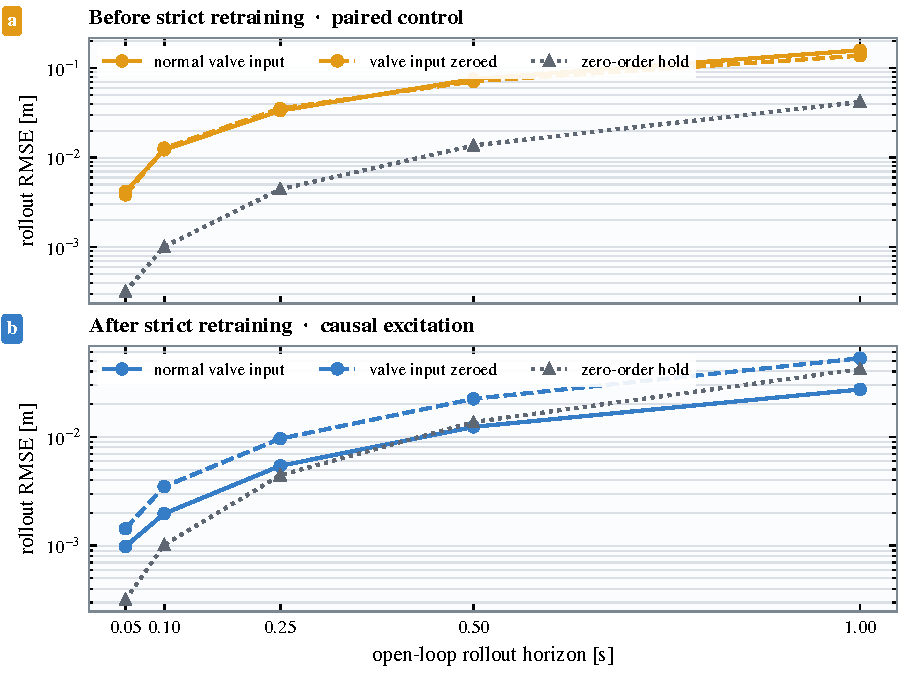
\includegraphics[width=\textwidth]{images/ch5_fd_rollout_authority}
  \caption{Open-loop extension rollout RMSE on held-out strict-excitation
  data as a function of rollout horizon, before (orange) and after (blue)
  strict retraining. Dashed curves show the same model with the valve input
  zeroed; the gap between solid and dashed is the model's usable valve
  authority. The paired-control FD is insensitive to its valve input,
  whereas the strict FD degrades by a factor of 1.8--1.9 when the valve is
  removed and outperforms the zero-order hold baseline (gray) beyond
  $\unit[0.5]{s}$.}
  \label{fig:models:fd-authority}
\end{figure}

Figure~\ref{fig:models:fd-authority} and Table~\ref{tab:models:fd-strict}
summarize the outcome. The strict FD reduces the $\unit[0.5]{s}$ extension
rollout RMSE from $\unit[75.2]{mm}$ to $\unit[12.4]{mm}$ and the
$\unit[1.0]{s}$ RMSE from $\unit[157.9]{mm}$ to $\unit[27.3]{mm}$, and ---
the decisive criterion --- its valve-zero error ratio rises from $0.94$ to
$1.81$ at $\unit[0.5]{s}$: removing the valve input now roughly doubles the
rollout error, which is exactly the sensitivity a control-relevant forward
model must exhibit. Per-axis one-step extension-increment $R^2$ improved
from the range $[-5.7,\, 0.60]$ to $[0.76,\, 0.98]$. Two honest limitations
remain. First, at very short horizons ($\leq \unit[0.25]{s}$) the zero-order
hold baseline is still competitive, because extension simply does not move
far in $\unit[0.05]{s}$; the learned model's value appears at the horizons
over which a target increment must be committed. Second, the
velocity-increment outputs remain poorly predicted (near-zero or negative
$R^2$ on two axes, dominated by relief transients that a memoryless
$\unit[0.05]{s}$ model cannot resolve). The deployed controller therefore
integrates only $\Delta\hat{\bm{x}}$, the accurately modeled and directly
validated quantity, and treats the velocity output as diagnostic.

\begin{table}[tb]
  \centering
  \caption{Strict-excitation validation of the FD model before and after
  strict retraining. The valve-zero error ratio is the rollout RMSE with
  zeroed valve input divided by the RMSE with the true valve input at a
  $\unit[0.5]{s}$ horizon; a ratio near 1 means the model ignores the valve.}
  \label{tab:models:fd-strict}
  \begin{tabular}{lcc}
    \toprule
    Metric & Paired-control FD & Strict FD \\
    \midrule
    Valve-zero error ratio at $\unit[0.5]{s}$ & $\approx 0.94$ & $1.81$ \\
    Extension rollout RMSE at $\unit[0.5]{s}$ & $\unit[75.2]{mm}$ & $\unit[12.4]{mm}$ \\
    Extension rollout RMSE at $\unit[1.0]{s}$ & $\unit[157.9]{mm}$ & $\unit[27.3]{mm}$ \\
    One-step $\Delta x$ $R^2$ (per-axis range) & $-5.7$ to $0.60$ & $0.76$ to $0.98$ \\
    \bottomrule
  \end{tabular}
\end{table}

For completeness, an intermediate rank-preserving fine-tuning stage between
the supervised and paired stages regularized the valve-to-extension
differential map with a finite-difference Jacobian penalty; the resulting
checkpoint has a full-rank (rank-4) valve Jacobian with condition number
$\approx 2.3$ and is retained as provenance, but the strict FD supersedes it
as the active model. The strict FD
(\texttt{best\_fd\_cylinder\_strict.pt}) together with the paired-control ID
constitutes the learned actuator pair of every PPO1 experiment in
Chapter~\ref{chap:evaluation}.

\section{Reduced-Order Model}
\label{sec:models:rom}

\subsection{Motivation and design position}

The PPO1 actuator path composes two separately trained networks and, as the
previous sections showed, needed three repair stages before the composition
had authority. The PPO2 path replaces the composition with a single
\emph{command-conditioned reduced-order model} that is trained end-to-end on
exactly the quantity the controller consumes: the response of the cylinders
to a desired cylinder command. Two design decisions distinguish the ROM from
a generic sequence model. First, it is \emph{grey-box}: pressure, force,
velocity, and extension are propagated through explicit physical update
equations with trainable effective parameters, and neural components only
supply what the physics cannot --- the valve realization, unmodeled load,
and bounded residual corrections~\cite{karniadakis2021physics,lutter2019deep}.
This follows the observation from Section~\ref{sec:models:fd} that valve
authority is strongly pressure-dependent: encoding the
orifice-flow--continuity structure~\cite{merritt1967hydraulic} makes that
dependence architectural rather than something to be rediscovered from data.
Second, it is \emph{recurrent}: a GRU encoder~\cite{cho2014learning} over
$0.25$~s of history replaces the memoryless state input of the FD, in the
spirit of the learned actuator networks of
Hwangbo et al.~\cite{hwangbo2019learning}, because hydraulic response
depends on recent pressure and command history that a single sample cannot
represent.

\subsection{Input--output contract}

The ROM consumes a history of $L=6$ samples ($\unit[0.25]{s}$ at
$T=\unit[0.05]{s}$) of the 24-dimensional feature vector
%
\begin{equation}
  \label{eq:models:rom-input}
  \bm{z}_k = \bigl[\bm{x}_k,\; \dot{\bm{x}}_k,\; \Delta\bm{p}_k,\;
  \hat{\bm{u}}_{k-1},\; \bm{c}_k \bigr] \in \mathbb{R}^{24},
\end{equation}
%
i.e.\ the cylinder state, the \emph{previously predicted} valve command fed
back as recurrent state, and the current desired command
$\bm{c}_k \in \mathbb{R}^8$ of \eqref{eq:models:command}. The actual valve
command appears only as a training target for the internal valve head; at
runtime no valve signal enters the model. From
$\mathcal{H}_k = (\bm{z}_{k-L+1}, \dots, \bm{z}_k)$ the ROM predicts the
internal valve realization and the full next cylinder state,
%
\begin{equation}
  \label{eq:models:rom-output}
  \bigl(\hat{\bm{u}}_k,\; \Delta\hat{\bm{p}}_k,\;
        \Delta\hat{\dot{\bm{x}}}_k,\; \Delta\hat{\bm{x}}_k\bigr)
  = f_{\mathrm{ROM}}\bigl(\mathcal{H}_k\bigr),
\end{equation}
%
which jointly replaces the ID--FD composition of the PPO1 path.

\subsection{Grey-box structure}

\begin{figure}[tb]
  \centering
  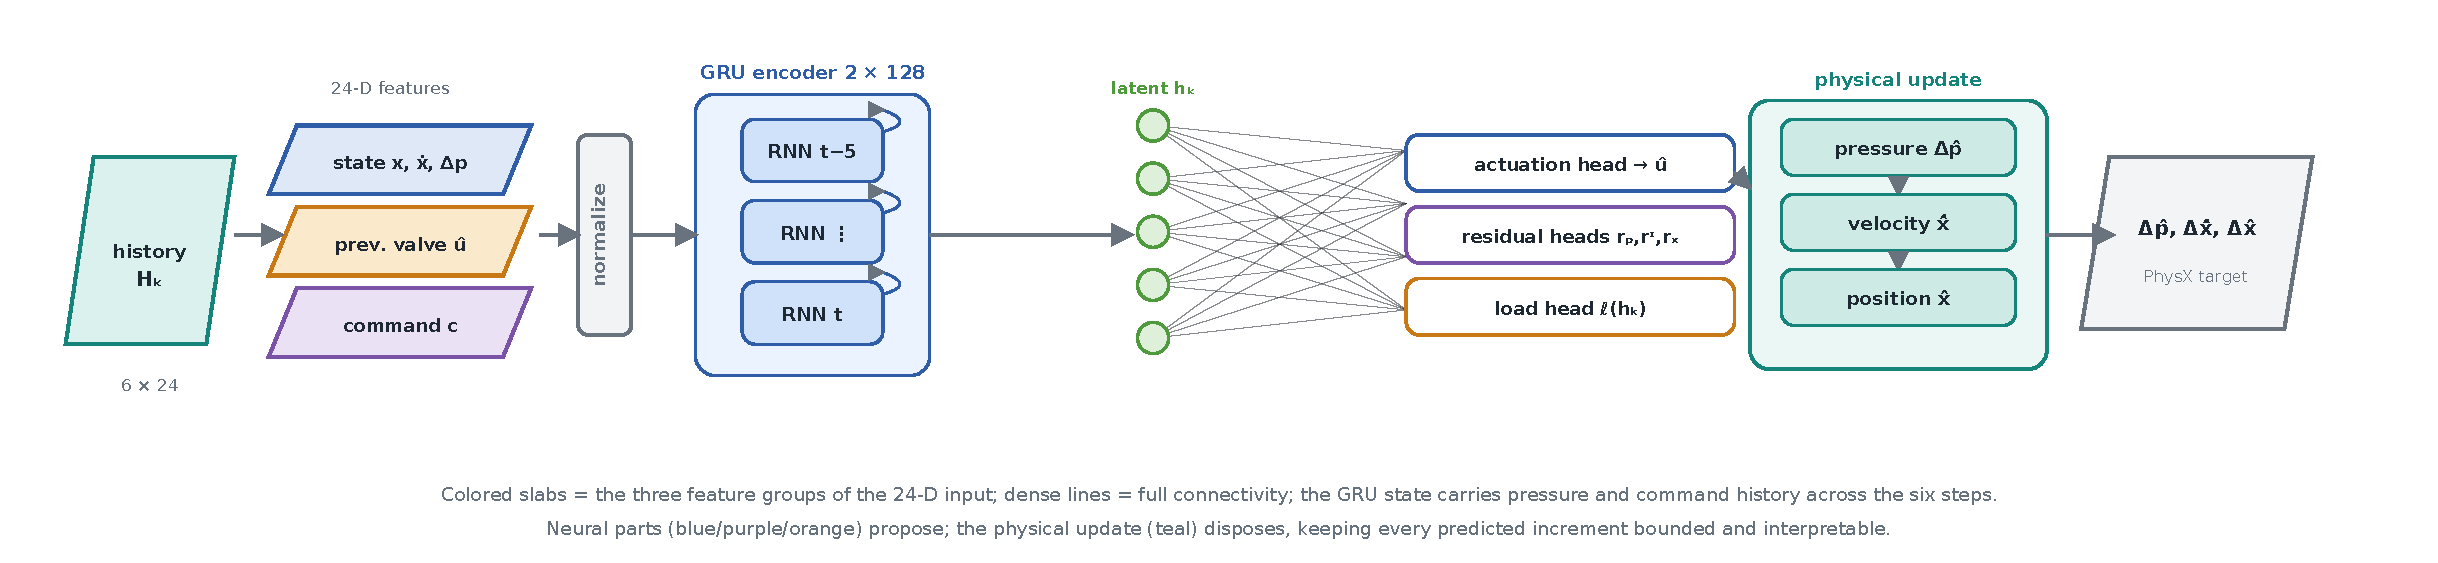
\includegraphics[width=\textwidth]{images/models_rom_pipeline}
  \caption{Structure of the command-conditioned reduced-order model as
  a data-flow pipeline. The $\unit[0.25]{s}$ history is split into its
  three feature groups (state, previously predicted valve, desired
  command), normalized, and passed through the recurrent GRU encoder
  whose hidden state carries pressure and command history across the six
  steps. The final latent feeds three fully connected heads: the
  actuation head realizes the command as an internal valve signal, the
  residual heads supply tanh-bounded corrections, and the load head the
  configuration load. The state is then propagated through the explicit
  pressure \eqref{eq:models:rom-pressure}, velocity
  \eqref{eq:models:rom-velocity}, and position
  \eqref{eq:models:rom-position} updates with trainable effective
  hydraulic parameters, so the neural parts propose and the physics
  disposes.}
  \label{fig:models:rom-structure}
\end{figure}

Figure~\ref{fig:models:rom-structure} shows the computation. The normalized
history is encoded by a two-layer GRU of width 128 (dropout $0.05$); the
final latent $\bm{h}_k$ and the command $\bm{c}_k$ feed a small actuation
head whose output passes through a learnable smooth dead-zone element ---
per-cylinder trainable width and asymmetric gains, built from softplus and
$\tanh$ primitives so it remains differentiable --- reflecting the dead band
and direction-dependent gain of proportional valves
(Section~\ref{sec:fund:actuation-chain}). The resulting
internal actuation $\hat{a}_i \in [-1,1]$ drives an orifice-flow and
continuity update per cylinder $i$,
%
\begin{align}
  q_i &= \hat{a}_i\, k_{q,i}\,
    \sqrt{\tfrac{1}{2}\bigl(p_{s,i} - \operatorname{sgn}(\hat{a}_i)\,
    \Delta p_i\bigr)_{+}}, \notag \\
  \Delta \hat{p}_{i,k+1} - \Delta p_{i,k} &=
    \frac{4\beta_i}{V_i(x_i)}
    \bigl(q_i - A_i \dot{x}_i - k_{\ell,i}\, \Delta p_i\bigr)\, T
    \;+\; r_{p,i},
  \label{eq:models:rom-pressure}
\end{align}
%
with effective bulk modulus $\beta_i$, supply pressure $p_{s,i}$, flow gain
$k_{q,i}$, leakage coefficient $k_{\ell,i}$, piston area $A_i$, and
extension-dependent chamber volume
$V_i(x_i) = V_{0,i} + A_i (x_i - x_{\mathrm{ref},i})$; the softplus-smoothed
pressure margin $(\cdot)_+$ keeps the square root differentiable near the
supply limit. The pressure then produces force, and force produces motion:
%
\begin{align}
  \hat{F}_i &= \Delta\hat{p}_{i,k+1} A_i + r_{F,i}, \qquad
  \ddot{x}_i = \frac{\hat{F}_i - c_{v,i}\,\dot{x}_i - \ell_i(\bm{h}_k)}{m_i},
  \notag \\
  \dot{\hat{x}}_{i,k+1} &= \dot{x}_{i,k}
    + \operatorname{sat}\bigl(T\,\ddot{x}_i + r_{v,i}\bigr),
  \label{eq:models:rom-velocity} \\
  \hat{x}_{i,k+1} &= x_{i,k}
    + \tfrac{T}{2}\bigl(\dot{x}_{i,k} + \dot{\hat{x}}_{i,k+1}\bigr)
    + r_{x,i},
  \label{eq:models:rom-position}
\end{align}
%
where $c_{v,i}$ is a viscous friction coefficient, $m_i$ an effective
modal mass, and $\ell_i(\bm{h}_k)$ a neural load head that captures the
configuration-dependent gravitational and coupling load. All physical
parameters are trained in log-space with hard clamps to physically plausible
ranges, so they can adapt to the data without leaving their meaning behind.
The trapezoidal position update \eqref{eq:models:rom-position} is the same
identity \eqref{eq:models:trapezoid} that the strict data satisfies almost
exactly. The neural residuals $r_{p}, r_{v}, r_{x}$ are $\tanh$-bounded to
10\,\% of the pressure step limit, 10\,\% of the velocity step limit, and
$\unit[1]{cm}$ respectively: large enough to absorb model error, too small
to let the network bypass the physics. This bounded-residual layering is
the central robustness argument of the grey-box design --- even a poorly
trained residual cannot produce an unphysical state jump.

\subsection{Dataset and training}

The command-ROM dataset joins the aligned ID and FD closed-loop exports on
exact run identifiers and time indices, yielding the $452\,400$
transitions and run-level 936/52/52 split summarized in
Section~\ref{sec:models:overview}; the logged valve commands enter only as
supervision for the internal valve head. Training (seed 17, Adam, learning
rate $3\times10^{-4}$, weight decay $10^{-5}$, batch size $2\,048$,
gradient-norm clipping at 5) follows a four-stage rollout curriculum with
horizons $H \in \{1, 5, 20, 50\}$ and stage lengths of $30/30/30/40$ epochs:
each stage optimizes the weighted one-step losses plus a recursive rollout
loss at its horizon, with scheduled sampling ramping from fully teacher-forced
to 75\,\% self-fed within each rollout~\cite{bengio2015scheduled}. The loss
weights (pressure $1.0$, velocity $2.0$, extension $1.0$, rollout $2.0$,
valve supervision $1.0$, residual penalty $0.1$, actuation regularization
$0.5$) penalize the residual heads explicitly so that explanatory burden
stays on the physical terms. The logged force channel receives zero
supervised weight: it failed a piston-area consistency audit on the current
curriculum ($F \neq \Delta p \cdot A$ within tolerance), and supervising a
head on a label that violates the model's own structure would corrupt the
pressure chain. The ROM still exposes its pressure-derived force
internally; force supervision can be enabled once a reliable chamber-force
label is available.

\begin{figure}[tb]
  \centering
  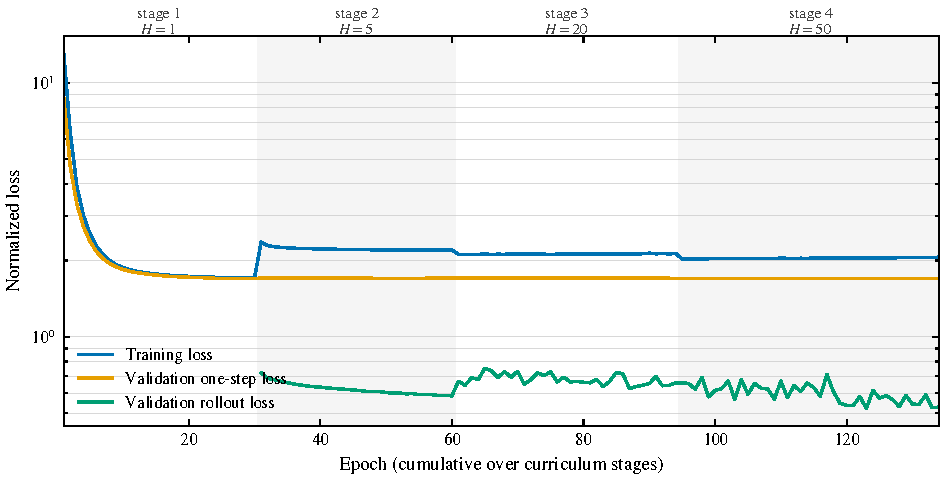
\includegraphics[width=\textwidth]{images/ch5_rom_training_history}
  \caption{Training history of the promoted command-ROM run over the
  four-stage rollout curriculum ($H$ is the recursive rollout horizon of
  each stage). The step in training loss at each stage boundary reflects
  the added longer-horizon rollout term; the validation one-step loss
  remains stable while the validation rollout loss continues to improve
  through stage~4.}
  \label{fig:models:rom-training}
\end{figure}

Figure~\ref{fig:models:rom-training} shows the resulting training history.
The characteristic step in the training loss at each stage boundary is the
newly added, harder rollout term; the important observation is that the
validation one-step loss does not degrade as longer horizons are introduced,
while the validation rollout loss improves --- the curriculum buys
long-horizon stability without sacrificing one-step accuracy.

\subsection{Offline validation}

\begin{figure}[tb]
  \centering
  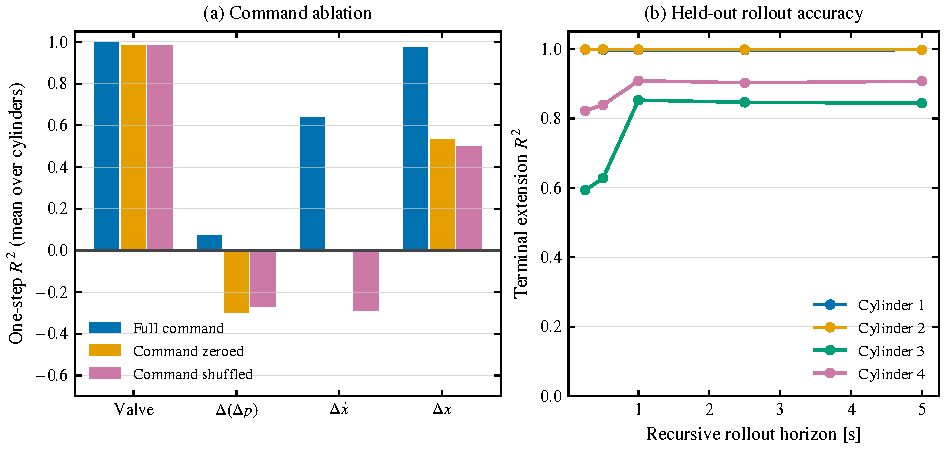
\includegraphics[width=\textwidth]{images/ch5_rom_validation}
  \caption{Offline validation of the command ROM on held-out runs.
  (a)~One-step $R^2$ per output group (mean over the four cylinders) with
  the full desired command, with the command zeroed, and with the command
  shuffled across the batch; the collapse of the velocity and extension
  scores without the true command demonstrates command authority.
  (b)~Terminal extension $R^2$ of recursive rollouts up to $\unit[5]{s}$
  (100 steps) per cylinder.}
  \label{fig:models:rom-validation}
\end{figure}

The offline acceptance report (4\,096 held-out samples, all gates passed) is
summarized in Figure~\ref{fig:models:rom-validation}. Three findings matter
for the control experiments. First, \emph{command authority}: with the true
command, mean one-step $R^2$ is $0.998$ for the internal valve prediction,
$0.64$ for the velocity increment, and $0.97$ for the extension increment;
zeroing or shuffling the command collapses the velocity score to below zero
and the extension score to $\approx 0.5$, and the $4\times4$ Jacobian of
predicted extension increment with respect to the commanded increment is
diagonally dominant with singular values $1.00$--$0.47$ and condition number
$2.14$. The model responds to what it is asked to do, per axis, which is
precisely the property whose absence broke the pretrained FD. Second,
\emph{rollout stability}: recursive rollouts remain accurate and bounded to
at least $\unit[5]{s}$ (terminal extension $R^2$ of $0.998$/$0.998$/$0.84$/
$0.91$ per cylinder), so PPO2 training rollouts do not ride on a diverging
model. Third, \emph{honest weaknesses}: the one-step pressure-increment
$R^2$ is low ($0.06$--$0.09$) --- pressure transients at $\unit[0.05]{s}$
resolution remain largely unpredictable, and the model's pressure state is
best understood as an internal latent that supports the velocity chain
rather than as a calibrated pressure estimator --- and cylinders 3 and 4
(boom~II and head pivot) are consistently harder than cylinders 1 and 2 in
both velocity and rollout scores. Inference costs $21.5\,\mu\mathrm{s}$ per
step in evaluation, which is compatible with the vectorized IsaacLab
training loop.

Beyond these aggregate scores, the acceptance protocol requires
pressure--velocity phase-plane checks, frequency-response comparisons, and
an in-simulator cylinder step gate before any PPO2 training run; a
state-only variant trained with the command zeroed throughout serves as the
mandatory comparison model for the identifiability ablations in
Chapter~\ref{chap:evaluation}. The nominal, randomized/robust, and
latent-conditioned ROM variants used in the PPO2-A/B/C experiments all share
the architecture and training protocol of this section and differ only in
their training distribution and conditioning inputs; the latent conditioning
mechanism is developed in Sections~\ref{sec:models:latent}
and~\ref{sec:models:aam}.

\section{Latent Representation of Randomized Dynamics}
\label{sec:models:latent}
% - How the teacher/encoder obtains a compact representation from
%   randomized-system context.
% - Latent dimension and training objective.
% - Latent clusters/trends vs. parameter variations — avoid
%   unsupported one-latent-one-parameter claims.
\todo{write}

\section{Arm Adaptation Module}
\label{sec:models:aam}
% - Observation history available online.
% - Temporal estimator predicting the teacher latent vector.
% - Causal deployment, update rate, warm-up history, behaviour after
%   sudden or gradual parameter changes.
\todo{write}

\section{Training and Model-Selection Protocol}
\label{sec:models:training}
% - Common train/validation/test splits.
% - Hyperparameters, early stopping, checkpoint selection, seeds.
% - Loss weighting across cylinder extension, velocity, pressure, or
%   other target groups.
\todo{write}

\section{Offline Model Evaluation}
\label{sec:models:offline-eval}
% - One-step and multi-step rollout metrics.
% - Nominal, randomized seen, unseen-parameter performance.
% - AAM latent-estimation error and adaptation delay.
% - Ablations: valve input, history length, latent conditioning,
%   dataset source.
\todo{write}

%%%%%%%%%%%%%%%%%%%%%%%%%%%%%%%%%%%%%%%%%%%%%%%%%%%%%%%%%%%%
%% Chapter 6 — Control Framework and Simulation Integration
%% (12–18 pages)
%% Purpose: explain the complete hierarchical controller and
%% present PPO1 and PPO2 as two controlled experimental
%% pipelines rather than a collection of disconnected models.
%% Main output: reproducible controller architecture, PPO task
%% definition, integration details, fair configuration of all
%% methods.
%%%%%%%%%%%%%%%%%%%%%%%%%%%%%%%%%%%%%%%%%%%%%%%%%%%%%%%%%%%%
\chapter{Control Framework and Simulation Integration}
\label{chap:control}

\section{Nominal Task-Space Controller}
\label{sec:ctrl:dls}
% - Reference-pose generation and task-space error.
% - DLS inverse differential kinematics and damping strategy.
% - Velocity/position-increment limits; mapping to cylinder targets.
% - DLS as nominal structured controller, not the adaptive contribution.
\todo{write}

\section{Residual PPO Formulation}
\label{sec:ctrl:ppo}
% - What PPO corrects: task-space commands, joint/cylinder targets, or
%   low-level commands.
% - Observation groups, action scaling, action filtering, temporal
%   history.
% - Reward terms: tracking, smoothness, stability, limits,
%   pressure/effort penalties, residual magnitude.
% - Training curriculum, episode termination, policy network, PPO
%   hyperparameters.
\todo{write}

\section{PPO1-A: Nominal ID-FD Pipeline}
\label{sec:ctrl:ppo1a}
% - ID and FD trained on nominal data; no AAM, no latent conditioning.
% - Purpose: nominal learned-dynamics baseline under residual PPO.
\todo{write}

\section{PPO1-B: Randomized/Robust ID-FD Pipeline}
\label{sec:ctrl:ppo1b}
% - ID and FD trained/fine-tuned with randomized and informative data;
%   no AAM on the FD.
% - Purpose: does data diversity alone improve the ID-FD pipeline?
\todo{write}

\section{PPO2-A: Nominal ROM Pipeline}
\label{sec:ctrl:ppo2a}
% - ROM trained on nominal data, used with the PPO2 policy architecture.
% - No latent conditioning and no AAM.
% - Purpose: baseline for the reduced-order architecture.
\todo{write}

\section{PPO2-B: Randomized/Robust ROM Pipeline}
\label{sec:ctrl:ppo2b}
% - ROM trained across randomized systems, no online latent
%   conditioning.
% - Purpose: isolate robustness from adaptation.
\todo{write}

\section{PPO2-C: AAM-Conditioned ROM Pipeline}
\label{sec:ctrl:ppo2c}
% - AAM estimates current latent dynamics from recent observations;
%   the latent estimate conditions the ROM online.
% - Purpose: complete proposed adaptive method.
\todo{write}

\section{Optional Oracle-Latent Diagnostic}
\label{sec:ctrl:oracle}
% - True simulation latent/context supplied to the ROM as an
%   upper-bound diagnostic only (PPO2-D).
% - Gap between oracle and AAM separates ROM capacity limitations from
%   adaptation-estimation limitations.
\todo{write}

\section{IsaacLab Integration and Timing}
\label{sec:ctrl:integration}
% - Control and physics time steps, action decimation, observation
%   timing, history-buffer updates.
% - Model inference order and handling of previous actions.
% - Device placement, vectorized environments, checkpoint loading,
%   runtime cost.
\todo{write}

\section{Stability and Constraint Handling}
\label{sec:ctrl:constraints}
% - Joint, cylinder, velocity, pressure, valve limits.
% - Action clipping, rate limits, termination conditions, numerical
%   safeguards.
% - How residual authority is bounded so PPO cannot completely
%   override the nominal controller.
\todo{write}

%%%%%%%%%%%%%%%%%%%%%%%%%%%%%%%%%%%%%%%%%%%%%%%%%%%%%%%%%%%%
%% Chapter 7 — Experimental Evaluation and Discussion
%% (18–28 pages)
%% Purpose: test the model and control hypotheses under matched
%% conditions, EXPLAIN the results rather than only reporting them,
%% and keep robustness, privileged-latent and adaptation claims apart.
%% Main output: the complete evidence chain from offline model quality
%% to closed-loop task performance and adaptation.
%%
%% Every experiment in this chapter evaluates exactly three rows:
%%   PPO-ROM            frozen: command ROM              adaptive: none
%%   PPO-ID-FD          frozen: control ID + strict FD   adaptive: none
%%   PPO-ID(AAM)-FD     frozen: control ID + strict FD   adaptive: AAM + bounded ID adapter
%% There are no other policy variants in the primary comparison.
%%%%%%%%%%%%%%%%%%%%%%%%%%%%%%%%%%%%%%%%%%%%%%%%%%%%%%%%%%%%
\chapter{Experimental Evaluation and Discussion}
\label{chap:evaluation}

\section{Hypotheses and Fairness Controls}
\label{sec:eval:hypotheses}
% - Restate RQ1--RQ5 as testable hypotheses H1--H5:
%   H1: SD_z(s,u,z_true) outperforms matched SD_0 and latent controls on
%       held-out extension and velocity rollouts (already supported).
%   H2: SD_z(s,u,z_hat) retains a statistically supported fraction of the
%       true-latent gain on reserved runs.
%   H3: the true-latent ID adapter improves frozen ID-FD, establishing
%       adapter capacity before AAM error is introduced.
%   H4: the AAM-latent adapter improves frozen ID-FD in paired held-out
%       episodes and approaches the true-latent oracle.
%   H5: adaptation improves mismatch recovery without materially
%       degrading the nominal domain or violating any of the eight gates.
% - Define BEFOREHAND what supports or rejects each hypothesis.
% - Fairness controls: paired factor configurations, terrain meshes, path
%   families, seeds, episode lengths and safety stops across all three
%   stacks; matched policy capacity and training budget.
\todo{write}

\section{Model-Level Experiments}
\label{sec:eval:model-level}
% - ID valve prediction and frozen-ID transfer across nominal,
%   hydraulic, mechanical, combined and held-out domains: report the
%   transfer gap AND the failure mode.
% - FD and ROM one-step and rollout prediction; valve-input ablations
%   and persistence baselines.
% - SD_0 vs SD_z(z_true) vs SD_z(z_hat); AAM latent estimation error and
%   temporal stability under fixed and changing factor configurations.
\todo{write}

\section{System Response}
\label{sec:eval:system-response}
% Matched steps, ramps, PRBS and task commands. Per cylinder: rise time,
% settling time, overshoot, steady-state error and gain; extension,
% velocity and pressure response; action/valve saturation; cross-axis
% coupling. This experiment must EXPLAIN why one stack tracks laterally
% or vertically better, not merely report that it does.
\todo{write}

\section{Delay}
\label{sec:eval:delay}
% Estimate command-to-pressure, command-to-velocity, pressure-to-velocity
% and, where meaningful, cylinder-to-tool response, using controlled
% transients, cross-correlation and frequency/phase analysis. Report
% actuator, environment and AAM-update latencies SEPARATELY. Do not label
% a static kinematic mapping as a temporal delay.
\todo{write}

\section{Nonlinearity}
\label{sec:eval:nonlinearity}
% Sweep command magnitude and sign, pressure, extension, velocity,
% payload, COM and arm posture. Quantify extension/retraction asymmetry,
% dead zone, saturation, pressure-dependent gain, load dependence,
% hysteresis and coupling from repeated PAIRED measurements only.
\todo{write}

\section{End-Effector and Mowing Performance}
\label{sec:eval:tracking}
% Same feasible path families and held-out terrain meshes for all three
% stacks. Report lateral and cut-height RMSE, MAE and p95; maximum and
% along-track error; transient settling after path changes; contact
% fraction; head alignment; impacts; terminations; results per family and
% per worst mesh. The eight-gate contract is the MINIMUM acceptance
% criterion, not a substitute for the full distributions.
\todo{write}

\section{Robustness and Generalization}
\label{sec:eval:robustness}
% In-range anchors, held-out combinations and DECLARED out-of-range
% stress tests. Add observation noise, action delay, sensor dropout,
% terrain shift, payload and COM changes. Separate interpolation from
% extrapolation. Report success rate, tracking degradation, saturation,
% safety terminations and adaptation recovery time relative to nominal.
\todo{write}

\section{Adaptation Ablations}
\label{sec:eval:ablations}
% For PPO-ID(AAM)-FD compare: deployable z-hat; privileged true z; zero,
% mean, shuffled and random latents; frozen ID without adapter; adapter
% without AAM history; shorter/longer history; slower latent update; and
% the optional policy conditioned on z-hat (declare the added input --
% it is NOT the same policy architecture).
% The AAM claim requires deployable z-hat to beat frozen PPO-ID-FD AND to
% approach the true-latent oracle on held-out configurations.
\todo{write}

\section{Statistics and Reporting}
\label{sec:eval:metrics}
% Predeclared primary metrics and seeds. Paired episodes, per-run
% summaries, paired bootstrap confidence intervals. Validation choices
% kept strictly separate from the untouched final test set. Report
% failure cases, worst-case meshes and effect sizes, not only pooled
% means or binary gate verdicts. Report inference cost and throughput.
\todo{write}

\section{Integrated Discussion}
\label{sec:eval:discussion}
% - Explain the MECHANISM behind each positive and negative finding:
%   dataset information, model structure, latent estimation quality,
%   action authority, actuator behaviour.
% - Keep architecture effects, robustness effects and adaptation effects
%   separate.
% - Does the policy mask weak actuator dynamics? Use the standing model
%   error, command magnitude/smoothness and model rollouts as evidence.
% - Include the negative results explicitly: ID-FD's contact failure, the
%   tracking cost of UNCONSTRAINED PPO fine-tuning after distillation,
%   earlier latent redundancy, and the need for wider matched excitation.
% - Report the anchored fine-tuning evidence as a matched before/after on
%   the SAME horizon and mesh set: the warm-start reference checkpoint has
%   never been gate-scored, so the "PPO improved on the student" claim is
%   currently supported by training metrics only, not by the gates.
% - Relate the findings back to the research gap of Chapter~\ref{chap:fundamentals}.
\todo{write}

\section{Threats to Validity}
\label{sec:eval:validity}
% - The deployment plant is itself a learned model (command ROM + PhysX),
%   and PPO-ROM's actuator IS that plant model. State plainly that this
%   makes PPO-ROM the reference condition rather than a third competing
%   approximator, and that the ROM alone was calibrated against PhysX
%   (Section~\ref{sec:models:rom-calibration}) while ID-FD was not.
% - That calibration used the PARKED shapes, not the moving-verge task,
%   so it is weakest under cutter-ground contact.
% - Simscape-to-IsaacLab abstraction mismatch; simulation-to-real limits.
% - Finite factor ranges, sparse design (118 runs, 16 reserved
%   configurations), incomplete operating coverage.
% - Policy stochasticity, model-identifiability limits, and the
%   measurement assumptions behind each gate threshold.
\todo{write}

%%%%%%%%%%%%%%%%%%%%%%%%%%%%%%%%%%%%%%%%%%%%%%%%%%%%%%%%%%%%
%% Chapter 8 — Conclusion and Outlook (4–7 pages)
%% Purpose: summarize what was established, answer the research
%% questions directly, and identify next steps without
%% introducing new experimental evidence.
%% Main output: concise final statement of contributions,
%% limitations, and future research directions.
%%%%%%%%%%%%%%%%%%%%%%%%%%%%%%%%%%%%%%%%%%%%%%%%%%%%%%%%%%%%
\chapter{Conclusion and Outlook}
\label{chap:conclusion}

\section{Summary of the Approach}
\label{sec:concl:summary}
% - Dataset, learned models, control pipelines, adaptation mechanism,
%   evaluation — in the same order as the thesis.
\todo{write}

\section{Answers to the Research Questions}
\label{sec:concl:answers}
% - One direct evidence-based answer per research question, RQ1--RQ5.
% - State where evidence is positive, mixed, or insufficient. RQ2 is
%   already answered positively for the PRIVILEGED latent; do not let
%   that answer leak into RQ3 or RQ4.
\todo{write}

\section{Main Contributions}
\label{sec:concl:contributions}
% - Restate only contributions demonstrated by the results.
% - Distinguish implemented engineering contributions from scientific
%   findings.
\todo{write}

\section{Limitations}
\label{sec:concl:limitations}
% - Simulation only; the deployment plant is itself a learned model.
% - Factor coverage: 6 factors, 118 runs, 16 reserved test
%   configurations -- a sparse design over a large space.
% - Identifiability limits: which factors are separable and which are
%   only reachable as a lumped coordinate.
% - Policy-optimization limits: unconstrained PPO fine-tuning traded
%   tracking for contact, so fine-tuning is admissible only under the
%   reference anchor of Section~\ref{sec:ctrl:anchored}. The anchor is a
%   principled restriction and NOT a certificate -- the Pinsker bound
%   (eq:ctrl:pinsker) is vacuous at the production horizon, so every
%   promotion still rests on the empirical gates. The fixed multiplier
%   is not dual-ascended, so one point of the Pareto front is sampled
%   rather than the constrained problem being solved.
% - Adaptation limits: the adapter is bounded and sits only at the ID
%   layer; the FD, the ROM and the policy remain frozen.
\todo{write}

\section{Future Work}
\label{sec:concl:future}
% - Real-system data collection and sim-to-real validation.
% - Widening the adapter beyond the ID layer, or joint refinement of
%   the actuator model and the AAM.
% - Uncertainty-aware or probabilistic latent adaptation.
% - Safety-constrained policy optimization and pressure-aware control.
% - Direct policy conditioning on z-hat as a first-class design rather
%   than an ablation (only when scientifically justified).
\todo{write}


%%%%%%%%%%%%%%%%%%%%%%%%%%%%%%%%%%%%%%%%%%%%%%%%%%%%%%%%%%%%
%% Appendices
%%%%%%%%%%%%%%%%%%%%%%%%%%%%%%%%%%%%%%%%%%%%%%%%%%%%%%%%%%%%
\appendix
%%%%%%%%%%%%%%%%%%%%%%%%%%%%%%%%%%%%%%%%%%%%%%%%%%%%%%%%%%%%
%% Appendices A–E (per the experimental plan)
%%%%%%%%%%%%%%%%%%%%%%%%%%%%%%%%%%%%%%%%%%%%%%%%%%%%%%%%%%%%

\chapter{System Parameters and Coordinate Mappings}
\label{app:system-parameters}
% Coordinate and SIGN conventions, joint/cylinder ranges, plant
% parameters, mapping validation, initial pose, simulation constants,
% and the exact rate of every layer (physics, policy, learned model,
% AAM update, logging).
\todo{write}

\chapter{Dataset Manifests and Factor Ranges}
\label{app:dataset}
% (a) Historical Simscape campaigns: parameter ranges,
%     trajectory-generation settings, run split, preprocessing.
% (b) IsaacLab adaptation collection: full run manifest, the six factor
%     ranges, per-domain draw seeds, segment structure, PRBS settings,
%     the 82/20/16 run-level split and its factor keys, and the frozen
%     dataset checksums.
\section{Trajectories}

Each run receives its own reference trajectory, sampled rather than
scripted. Between twelve and twenty waypoints are drawn by Latin
hypercube sampling within the joint limits, and the arm moves between
them without dwelling, so that the data contains transitions rather than
long static holds. Segment durations are drawn from four speed classes,
slow ($1.5$--$\unit[2.5]{s}$), medium ($0.8$--$\unit[1.5]{s}$), fast
($0.3$--$\unit[0.7]{s}$), and variable ($0.5$--$\unit[2.5]{s}$), and
about a third of the runs receive additional exploratory perturbations
on top of the waypoint path.

An earlier version of this generator used four to eight waypoints with
dwell periods between them. It produced data in which the arm was
stationary for a large fraction of the time, which flatters any model
that learns to predict persistence. The current settings were chosen to
remove that easy mass of near-static samples, and the increase in
waypoint count is the single change that most improved the usefulness of
the batch.




\section{Execution and Logging}

Each run simulates $\unit[22]{s}$ of operation. The solver is the stiff
implicit \texttt{ode23t} integrator in accelerator mode with relative
and absolute tolerances of $10^{-2}$ and $10^{-3}$. The loose tolerances
are a deliberate throughput compromise, and their effect is bounded by
the consistency checks of Section~\ref{sec:data:diagnostics}. Output is
written on a fixed $\unit[0.05]{s}$ grid, giving 441 logged samples per
run, and the batch is checkpointed to disk every hundred runs so that a
failure late in a multi-day batch does not cost the whole collection.

For every run the archive stores the time vector, the five valve
commands, the four cylinder extensions, the four chamber pressure
differences, the four rod forces, the five joint positions and
velocities, the reference position and velocity signals, and, crucially,
the complete parameter structure that produced the run. That last item
is what makes the batch usable for the latent-adaptation work: the
privileged plant descriptor $\bm{\xi}$ of
Section~\ref{sec:fund:domain-randomization} is not something that has to
be reconstructed later, it is recorded alongside the trajectory.

The cost quantifies the argument made in
Section~\ref{sec:fund:sim-data-source}. A single
$\unit[64]{s}$ open-loop run takes roughly $\unit[2000]{s}$ of wall time
on the collection machine, a real-time factor of about $0.03$. The
Simscape plant runs some thirty times slower than the machine it
models. No policy-optimisation loop that needs millions of environment
steps can be built on that, which is why the learned actuator
surrogates exist.



\section{Parameter Ranges and Dataset Audit}

\begin{table}[htbp]
  \centering
  \caption{Randomized hydraulic parameters. The seal-wear coordinate is
  drawn independently for each of the four cylinders and drives three
  physically linked quantities at once.}
  \label{tab:data:hydraulic}
  \small
  \begin{tabular}{llll}
    \toprule
    Parameter & Nominal & Randomized range & Acts on \\
    \midrule
    Entrained air fraction $\varepsilon_{\mathrm{air}}$
      & $0.005$ & $0.001$ -- $0.080$ & fluid compliance \\
    Dead-volume fraction $\varepsilon_{\mathrm{vol}}$
      & $0.020$ & $0.005$ -- $0.080$ & fluid compliance \\
    Discharge coefficient $c_d$
      & $0.70$ & $0.56$ -- $0.84$ & valve flow gain \\
    Seal wear $w_{\mathrm{seal},i}$
      & $0$ & $0$ -- $0.25$ (per cylinder)
      & clearance, leakage, spool lag \\
    Relief setting $p_{\mathrm{set}}$
      & $\unit[27.6]{MPa}$ & $\unit[24.8]{MPa}$ -- $\unit[30.4]{MPa}$
      & pressure ceiling \\
    \bottomrule
  \end{tabular}
\end{table}

\begin{table}[htbp]
  \centering
  \caption{Randomized mechanical parameters. The rigid-body
  perturbations are applied independently to each of the fourteen
  bodies.}
  \label{tab:data:mechanical}
  \small
  \begin{tabular}{lll}
    \toprule
    Parameter & Nominal & Randomized range \\
    \midrule
    Body mass & CAD value & $\pm 20\,\%$ \\
    Centre-of-mass offset & CAD value & $\pm 5\,\%$ \\
    Inertia tensor and products & CAD value & consistent with mass draw \\
    Joint stiffness, J1 and J2 & $\unit[60]{kN/m}$ & $40$ -- $\unit[120]{kN/m}$ \\
    Joint stiffness, J3 and J4 & $\unit[60]{kN/m}$ & $40$ -- $\unit[120]{kN/m}$ \\
    Joint stiffness, J5 & $\unit[25]{kN/m}$ & $15$ -- $\unit[60]{kN/m}$ \\
    Joint damping & $250$ & $100$ -- $600$ \\
    \bottomrule
  \end{tabular}
\end{table}

\begin{table}[htbp]
  \centering
  \caption{The six randomized physical factors of the IsaacLab
  adaptation collection and their final ranges. One factor vector is
  drawn per run and held fixed for the whole run.}
  \label{tab:data:factors}
  \small
  \begin{tabular}{llll}
    \toprule
    Coordinate & Range & Domain & Acts on \\
    \midrule
    $e_{\mathrm{flow}}$       & $[-0.25,\, 0.25]$ & hydraulic  & valve flow gain \\
    $e_{\mathrm{compliance}}$ & $[-0.25,\, 0.10]$ & hydraulic  & effective chamber compliance \\
    $e_{\mathrm{seal}}$       & $[0,\, 1]$        & hydraulic  & seal wear, leakage, spool lag \\
    $e_{\mathrm{pressure}}$   & $[-0.15,\, 0.15]$ & hydraulic  & supply/relief pressure level \\
    $e_{\mathrm{mass}}$       & $[0.8,\, 1.5]$    & mechanical & cutter mass scale \\
    $e_{\mathrm{COM}_z}$      & $[-0.10,\, 0.05]$ & mechanical & cutter centre-of-mass height \\
    \bottomrule
  \end{tabular}
\end{table}

\begin{table}[htbp]
  \centering
  \caption{Audit of the strict open-loop excitation export. All checks
  are computed by the extraction stage and stored with the data; the
  export is accepted only if every one of them passes.}
  \label{tab:data:audit}
  \small
  \begin{tabular}{lll}
    \toprule
    Check & Result & Interpretation \\
    \midrule
    Rows, runs, columns & $25\,600$ / $4$ / $49$ & four complete runs \\
    Median sample time & $\unit[0.01]{s}$ & as commanded \\
    Maximum sample-time error & $9.1\times10^{-15}\,\mathrm{s}$ & numerically exact grid \\
    Maximum $\Delta$extension error & $0$ & targets match state differences \\
    Maximum $\Delta$velocity error & $0$ & targets match state differences \\
    Maximum $\Delta(\Delta p)$ error & $\unit[0]{Pa}$ & targets match state differences \\
    Non-finite values & $0$ & no solver escapes \\
    Valid fraction & $0.937$ & startup, gaps, shutdown excluded \\
    Command rank & $4$ & all four channels independent \\
    Lagged excitation rank & $80$ & history matrix full rank \\
    Valve saturation & $8.5\,\%$ per channel & limits reached but not dominant \\
    Stroke coverage & $12\,\%$ -- $33\,\%$ & above floor, below target \\
    \bottomrule
  \end{tabular}
\end{table}


\chapter{Model Architectures, Normalizers and Checkpoint Hashes}
\label{app:models}
% Layer definitions and input masks for command ROM, ID, strict FD,
% SD_0, the factor encoder mu(e), SD_z, the AAM and the ID adapter.
% Normalization statistics, loss weights, optimizers, schedules,
% checkpoint selection, and the SHA-256 hash of every frozen artifact.
% State explicitly for each model whether it is frozen or trained from
% scratch.
\todo{write}

\chapter{PPO and IsaacLab Configuration}
\label{app:ppo-config}
% The complete 66-D observation layout group by group, the four-action
% contract with per-cylinder scales and lead caps, all ten reward terms
% with weights, termination rules, the eight gates with their
% thresholds and the measurement each is anchored to, environment
% settings, and the full PPO hyperparameter set copied from the frozen
% experiment manifest.
\todo{write}

\chapter{Supplementary Results}
\label{app:results}
% Per-cylinder and per-seed results, per-path-family and per-mesh
% tables, additional trajectories, failure cases, extended ablations.
\todo{write}


%%%%%%%%%%%%%%%%%%%%%%%%%%%%%%%%%%%%%%%%%%%%%%%%%%%%%%%%%%%%
%% Bibliography
%%%%%%%%%%%%%%%%%%%%%%%%%%%%%%%%%%%%%%%%%%%%%%%%%%%%%%%%%%%%
\RRLABbibliography{literature}

\end{document}
